\chapter{Experimental setup}
This chapter intends to give a overview of the experimental set-up which was used to obtain cross section measurement. The facility of the Lawrence Berkeley National Laboratory's 88-Inch cyclotron is described in section \ref{sec:LBNL-88}, and the description of the experiment is described in section \ref{sec:experiment}, where the stacked target design technique, characterization and mounting of foils is described in subsection \ref{subsec:target_design} and the irradiation including tuning of the beam is described in subsection \ref{subsec:irradiation}. The analysis, including unfolding of the gamma-ray spectra is describes in chapter \ref{chapter:analysis}. 

%The thin foil stacked-target technique was applied to measure the experimental cross sections for reactions induced in iridium, iron, nickel and copper with deuteron energies ranging from ca. 33-5 MeV. This method is well-described in literature \footnote{https://sci-hub.tw/https://doi.org/10.1016/j.nimb.2016.09.018}\footnote{Niobium paper and iron paper from Andrew} for protons. This is however the first experiment using deuterons and the results may differ as for instance the deuteron break up effect is unknown. 

\section{Lawrence Berkeley National Laboratory's 88" Cyclotron} \label{sec:LBNL-88}

Lawrence Berkeley National Laboratory (LBNL) is a national research laboratory on behalf of the U.S. Department of Energy through its Office of Science, and is operated by University of California, Berkeley. LBNL was founded by Ernest Orlando Lawrence, the inventor of the cyclotron, in 1931.  \footnote{https://www.lbl.gov/about/}. The 88-Inch Cyclotron (K=140) has many purposes, and can accelerate both light and heavy ions up to Uranium. \footnote{http://cyclotron.lbl.gov/home}. The researchgroup inwhich does isotope production at the facility works with development of nuclear data, along with researching production methods of medically valuable radionuclides (site andrew articles?)  %The cyclotron number is the maximum kinetic energy which can be reached for protons (with no relativistic factors taken into account). The maximum kinetic energy a particle can gain is found from the cyclotron number:%\begin{equation}
%    \frac{E_k}{A}=K\Big(\frac{Q}{A}\Big)^2
%\end{equation}
%For deuterons with mass number A=2 and charge Q=1, the maximum kinetic energy is $E_k=70$ MeV. 
But there are multiple programs that takes place in the facility\footnote{https://ieeexplore.ieee.org/abstract/document/7999622/authors#authors} which include chip testing and space effects testing, super heavy element searches, fundamental nuclear structure measurements, novel scintillation characterization, fission yield and neutron inelastic scattering measurements (GENESIS) (from Andrew). \\
\noindent 
A cyclotron is a device that accelerates positively charged particles. It is operated by an alternating (radiofrequency) electric field, and a perpendicular magnetic field, which by the Lorentz Force forces the particle to accelerate in an outward spiral. The ions which are accelerated are produced by ECR ion sources and injected into the cyclotron \cite{KireeffCovo2018a}. The facility is figured in \ref{fig:LBNL_88}, and consists of a cyclotron vault and 5 experimental caves, where cave 0 is used for isotope production, neutron beams and chemistry \cite{Andrew HFNG article?}, which is where the irradiation of the target stack took place. Cave 4C is today used for gamma-ray spectroscopy, where 6 of a total of 7 high purity germanium detectors which were used in this work were located. Faraday cups (not in figure) can measure the beam current at different steps along the tube, which makes it possible to measure the transition efficiency of the beam. Faraday cups are dense metal block, usually 6-7 cm broad Copper and Tantilum. It works as a beam stopper, and can be lowered into the beam line to measure the current. Since it is electrically isolated, it is possible to measure the current, since we know the number of initial particles accelerated. Since to electrons close to the surface can be scattered of, it can read of higher positive charge than what is correct. Therefor, a magnet surrounds the cup to bend the electrons back to the Faraday cup in what is called magnetic suppression. Cave 0 is used mainly for neutron beam, chemistry, and isotope production, and was used for irradiation of the target stack. 


\begin{figure}
    \centering
    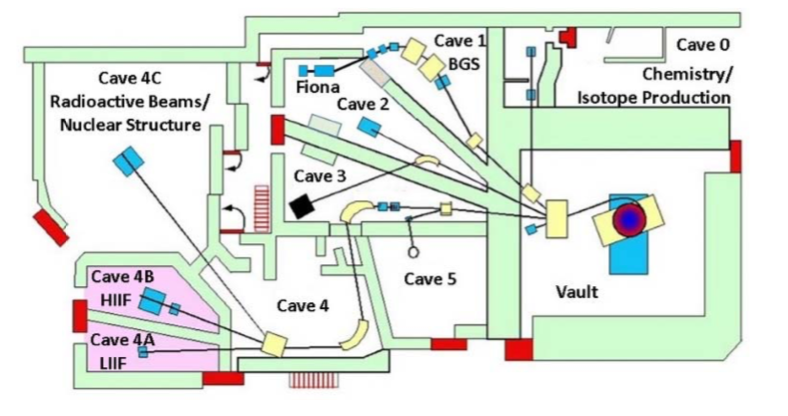
\includegraphics[width=0.8\textwidth]{Experiment/LBL_88.png}
    \caption{An overview of the 88" Cyclotron facility. https://cpb-us-e1.wpmucdn.com/sites.usc.edu/dist/7/89/files/2018/04/133-18q03um.pdf }
    \label{fig:LBNL_88}
\end{figure}

\section{Detector calibration} \label{sec:detector_calibration}
\noindent  

For the gamma-ray spectroscopy, seven different detectors were used; six IDM Ortec detectors (detectors 1-6) with detector diameter 85 mm, detector length 30 mm and hole depth 15 mm, and one Germanium detector (detector 7) with detector diameter 64.9 mm, detector length 57.8 mm and hole depth 48.6 mm \textcolor{red}{from detector diagrams}. The IDM-detectors were located in cave 4c (see figure \ref{fig:LBNL_88}), which have previously been used as radiation chamber. Thus, background radiation was present. For detector 7, there was led shielding around the detector. Spectra taken on the Germanium detector was preferred \textcolor{red}{explain the shape and geometry, wait from answer from andrew}. In order to visualize the signal from the detector, Maestro  (Multichannel Analyzer Emulation Software\footnote{https://www.ortec-online.com/products/application-software/maestro-mca}) was used. \\

High purity Germanium detector is a type of semiconductor, which is a material where the energy required to remove an electron from the valence band (in the outer atomic shell) to the conduction band is small. The germanium atom has atomic number 32, and 4 valence electrons in the outer p4 shell \textcolor{red}{(need citation?)}. The atoms in the detector are bound through covalent bonds in a crystal structure. The main mechanism of a semiconductor is creation of electron-hole pairs after energy deposition of an ionizing particle in the crystal. If an electron is excited to the conduction band, a hole is left. This hole can move as a neighboring electron fills this spot, and it can cause a chain reaction, and the hole will move in the crystal. Both the electron in the conduction band and the hole in the valence band contributes to an electric current. Under influence of an electric field, the electron-hole pairs will be collected and incident can be measured as a count. The major
advantage with semiconductor detector is that the average energy to create an electron-hole pair is
very low, which results in a superior energy resolution in comparison to other detectors like gas and
scintillation detectors. High energy resolution is important, dependent on the energy difference of two close lying gamma-peaks and the resolution, the two peaks can be distinguished. For 1000 keV, the resolution of a Germanium detector is 0.1\%, which means that it is possible to separate two gamma-ray peaks within ca. 1 MeV (\cite{Leo1994}, p. 117). At room temperature, thermal
energy can excite the electron from the valence to the conduction band and cause noise in spectra.
Therefor, Germanium detectors are operated at 0 Kelvin. Write about recombination and trapping,
noise, np semiconductor junction, depletion depth?? (\cite{Leo1994}, p. 215-216). \\

\noindent 
The electrical signal registered in a detector has a net-electrical charge which is proportional to the amount of gamma-ray energy which was registered in the detector (\cite{Gilmore2008}, p. 61). The electrical signal is assigned a channel number, which is in accordance with the charge collected. To obtain a spectrum, the number of registered events in each channel is counted, and the well-known peaks of the gamma-ray spectrum rises. Ideally, the peaks would appear as step functions, as the gamma-ray energies are discrete. Ionizing radiation statistics is based upon Poisson statistics, where the probability of observing N evens is a discrete value

\begin{equation}
    P(N)=\frac{\mu^N e^{-\mu}}{N!}
\end{equation}

where $\mu$ is the mean value, which is equal to the variance ($\mu=\sigma^2$). This distribution is valid when the probability is small \textcolor{red}{(decay probability small?)} and the number of trials (\textcolor{red}{number of decays?}) are large (\cite{Leo1994}, p. 85).  The distribution is not symmetric, but as the mean value increases, the peak approximates a Gaussian shape. Therefor the peak is assumed Gaussian with an exponential skew towards lower energies which is caused by incomplete charge collection, along with a step function which takes the background into account. The area of the whole peak is net net number of counts which is necessary to obtain an activity in the foil. The statistical uncertainty arises from the Poisson statistics, and is large if net number of counts are low:

\begin{equation}
    \sigma N_i = \sqrt{N_i}
\end{equation}

Therefor, to reduce the statistical uncertainty, a relative uncertainty of less than 1\% is preferred ($\frac{\sigma N_i}{N_i}\frac{1}{\sqrt{N_i}}=1\%$) 
The systematic uncertainty is in the detector, caused by a process called annealing. \textcolor{red}{write about it??}
%Unfortunately, the resolution of a detector is not that good. High energy resolution is important, dependent on the energy difference of two close lying gamma-peaks and the resolution, the two peaks can be distinguished (\cite{Leo1994}, p. 117). The peak arises is not directly Gaussian. 
%The way inwhich a detector can transform the electric signal from the detector to a  


\subsection{Energy and peakshape calibration}  \label{subsec:energy_peakshape_calibration}
Since the channel number is not analogous to the gamma-ray energy, the detector needed to be calibrated. The gamma-ray calibration pointsources  $^{137}$Cs ($t_{1/2}=30.08$ years\cite{Browne2007}), $^{133}$Ba ($t_{1/2}=10.551$ years\cite{Khazov2011}) and $^{152}$Eu ($t_{1/2}=13.517$ years\cite{Martin2013}) which were used can be seen in figure \ref{fig:calsources}. The calibration sources have very well-known gamma-energies, and by comparing the shift in the centroid of the peak in the spectrum to the true gamma-ray peak, a relationship can be developed. The gamma-lines which were used in the calibration are listed in table \ref{table:calibration_gammas}. The sources were counted so that the weakest line which was used had a statistical uncertainty of less than 1\% \textcolor{red}{double check}. The relationship between channel number and energy fits a straight line quite well, using two calibration points, \textcolor{red}{but whether this is a good approximation is dependent on the integral linearity of the gamma spectroscopy system} 
\begin{equation}
    E = a+b\cdot C
\end{equation}
where a is the slope of the line, b is the intercept and c is the channel number at that energy. 
(\cite{Gilmore2008} p. 145, for both statements) \\

\noindent 
In this work, the gamma-ray spectra were analyzed in FitzPeaks\footnote{https://www.jimfitz.co.uk/fitzpeak.htm}. The mathematical algorithm inwhich Fitzpeaks in based on is SAMPO80\cite{Koskelo1981}. In this algorithm, the peaks are assumed Gaussian joined with an exponential tale on both sides of the peak, so that the function and first derivative are continuous. The peak search utilizes the smooth second difference \textcolor{red}{derivative?}, which makes it a good algorithm for detecting small peaks on low background\cite{Koskelo1981}. The peak areas are calculated by fitting the precalibrated modified Gaussian to the data with a weighted least squares formula using a parabolicbackground \cite{THE ARTICLE HERE, but what page??}.  Fitting intervals are determined automatically by the program.  Peaks separarated byless than 4 times the average fwhm are fitted together. In FitzPeaks, peak shape and energy calibration was done, by first fitting the calibration spectra taken for each detector, and  supplying energy and peak shape source files for the gammarays listed in the table for the specific source. This way, each detector was calibrated. For the peak shape, the program optimizes seven parameters; two background peaks, the peak height and location, the peak width, the distance from the peak centroid to the starting point of the exponential tale on either side (\cite{Koskelo1981}, p. 90). 
For the energy calibration, linear interpolation (\textcolor{red}{with two optimizing parameters, a,b}) on a linear scale is used. The minimization of the optimized parameters are performed using an iterative gradient method. \textcolor{red}{include more??}  Calibration errors are added to the peak location and intensity errors to give the final result (\cite{Koskelo1981}, p. 94). 
 


\noindent 
\subsection{Efficiency calibration}
The efficiency of the detector is dependent on the shape and density of the detector (\cite{Gilmore2008}, p. 144), and is a very important parameter in the calculation of the end of beam activities from equation \ref{eq:Final_Expression_A0}. The efficiency of a detector is the number of events registered divided by the events emitted by the source. The absolute efficiency can be divided into intrinsic and geometrical efficiency, where the intrinsic efficiency is the number of events registered by the number of events hitting the detector. The intrinsic efficiency thus depends on the interaction cross section between the incident particle and the detector material. For neutral particles like photons, the size affects the intrinsic efficiency, as the probability of interaction gets larger. The geometrical efficiency is based upon the shape, and is the radiation emitted by the source which hits the detector (\cite{Leo1994}, p. 121-122).\\ 

The same calibration point sources which were used in the energycalibration were used in the efficiency calibration, with the same gammas which are listed in table \ref{table:calibration_gammas}. On each calibration source (figure \ref{fig:calsources}) a reference date given with an activity, which here is referenced to as $A_0$ of the calibration sources. \noindent Solving Equation \ref{eq:Final_Expression_A0} for effiency, $\epsilon$, the analytical effiency as a function of gamma-ray energy and intensity is 
\begin{equation} \label{eq:efficiency_analytical}
    \epsilon(E_\gamma)= \frac{N_C \lambda}{A_0 I_\gamma (1-e^{-\lambda \Delta t_c})e^{-\lambda\Delta t_d}}
\end{equation}

\noindent 
where $\lambda$ is the decay constant and $N_C$ is the number of counts in the measured spectra, and $\Delta t_d$ is the delay time since the reference date. The analytical efficiency gives one single value for the efficiency at energy $E_\gamma$, but we want a continuous function which gives the efficiency at any gamma-energy. A model based upon Gallagher, W. J., Cipolla, S.J. (1974)\cite{Gallagher1974b} \textcolor{red}{also cite amanda and eric once reference exists} was applied which takes the probability of penetration through the deadlayer of the detector and the probability of interaction in the detector volume into account

\begin{equation} \label{eq:efficiency_estimated}
\epsilon(E_\gamma) =  B_0 + \underbrace{(e^{-B_1 E_\gamma^{B_2}})}_\text{dead layer}  \underbrace{(1-e^{-B_3 E_\gamma^{B_4}}))}_\text{interacting with volume} 
\end{equation}
\noindent 
where $B_i$ is optimization parameters. The scipy optimize curvefit function \cite{Virtanen2020} takes in the analytically calculated efficiencies and uncertainties calculated from equation \ref{eq:efficiency_analytical}. \textcolor{red}{Not 100\% sure: was the uncertainty for each individual measurement calculated as they were uncorrelated, and the total uncertainty as if they wer correlated?} The uncertainty in each parameter was accounted for correlations, and calculated according to equation \ref{eq:variance_full}. Then, to estimate the curve, the function finds the optimal parameters of $B_i$ minimizing the $\Chi^2$ (equation \ref{eq:chisq}). Figure \ref{fig:efficiency_curve} shows an example of an efficiency curve for a detector at a specific distance from the detector. The uncertainty of the efficiency was estimated using equation \ref{eq:variance_full} numerically, where low uncertainties weight the fit. For each source, the gamma-lines with the intensities which were used to calculate the efficiency points for each source is listed in table \ref{table:calibration_gammas}. Figure \ref{fig:efficiency_curves} shows two different efficiency curves. The top figure shows the efficiency curve for detector one at a distance 30 cm from the detector surface, and the bottom figure shows the efficiency curve for detector 7 av 5 cm from the detector surface. For the former, the curve follows the points around the peak very well. For the latter, the model has a harder time fitting the peak, which is due to the high uncertainty of the $^{137}$Cs peaks. It is clear that the fit weights the low-uncertainty points. One of the reasons that some of the points in detector 1 have large uncertainties is due to the detector geometry and the increasing distance from the detector. The two first peaks of $^{137}$Cs also differs in comparison to each other. The lines which were used are X-rays, which are difficult to fit, and are relatively low in intensity. In addition, the gamma-ray energy region has a high slope in efficiency which makes it difficult to fit exactly.  All the uncertainties which are remarkably higher than others have intensities of less than 1\%. This could have been avoided by excluding these low-intensity gamma-lines, but since the fit is uncertainty-weighted, the number of lines remained. On both figures, the uncertainty is higher around the peak, and for detector 7 the uncertainty is increasing with energy.   \\


\begin{figure}%
    \centering
    \subfloat[]{{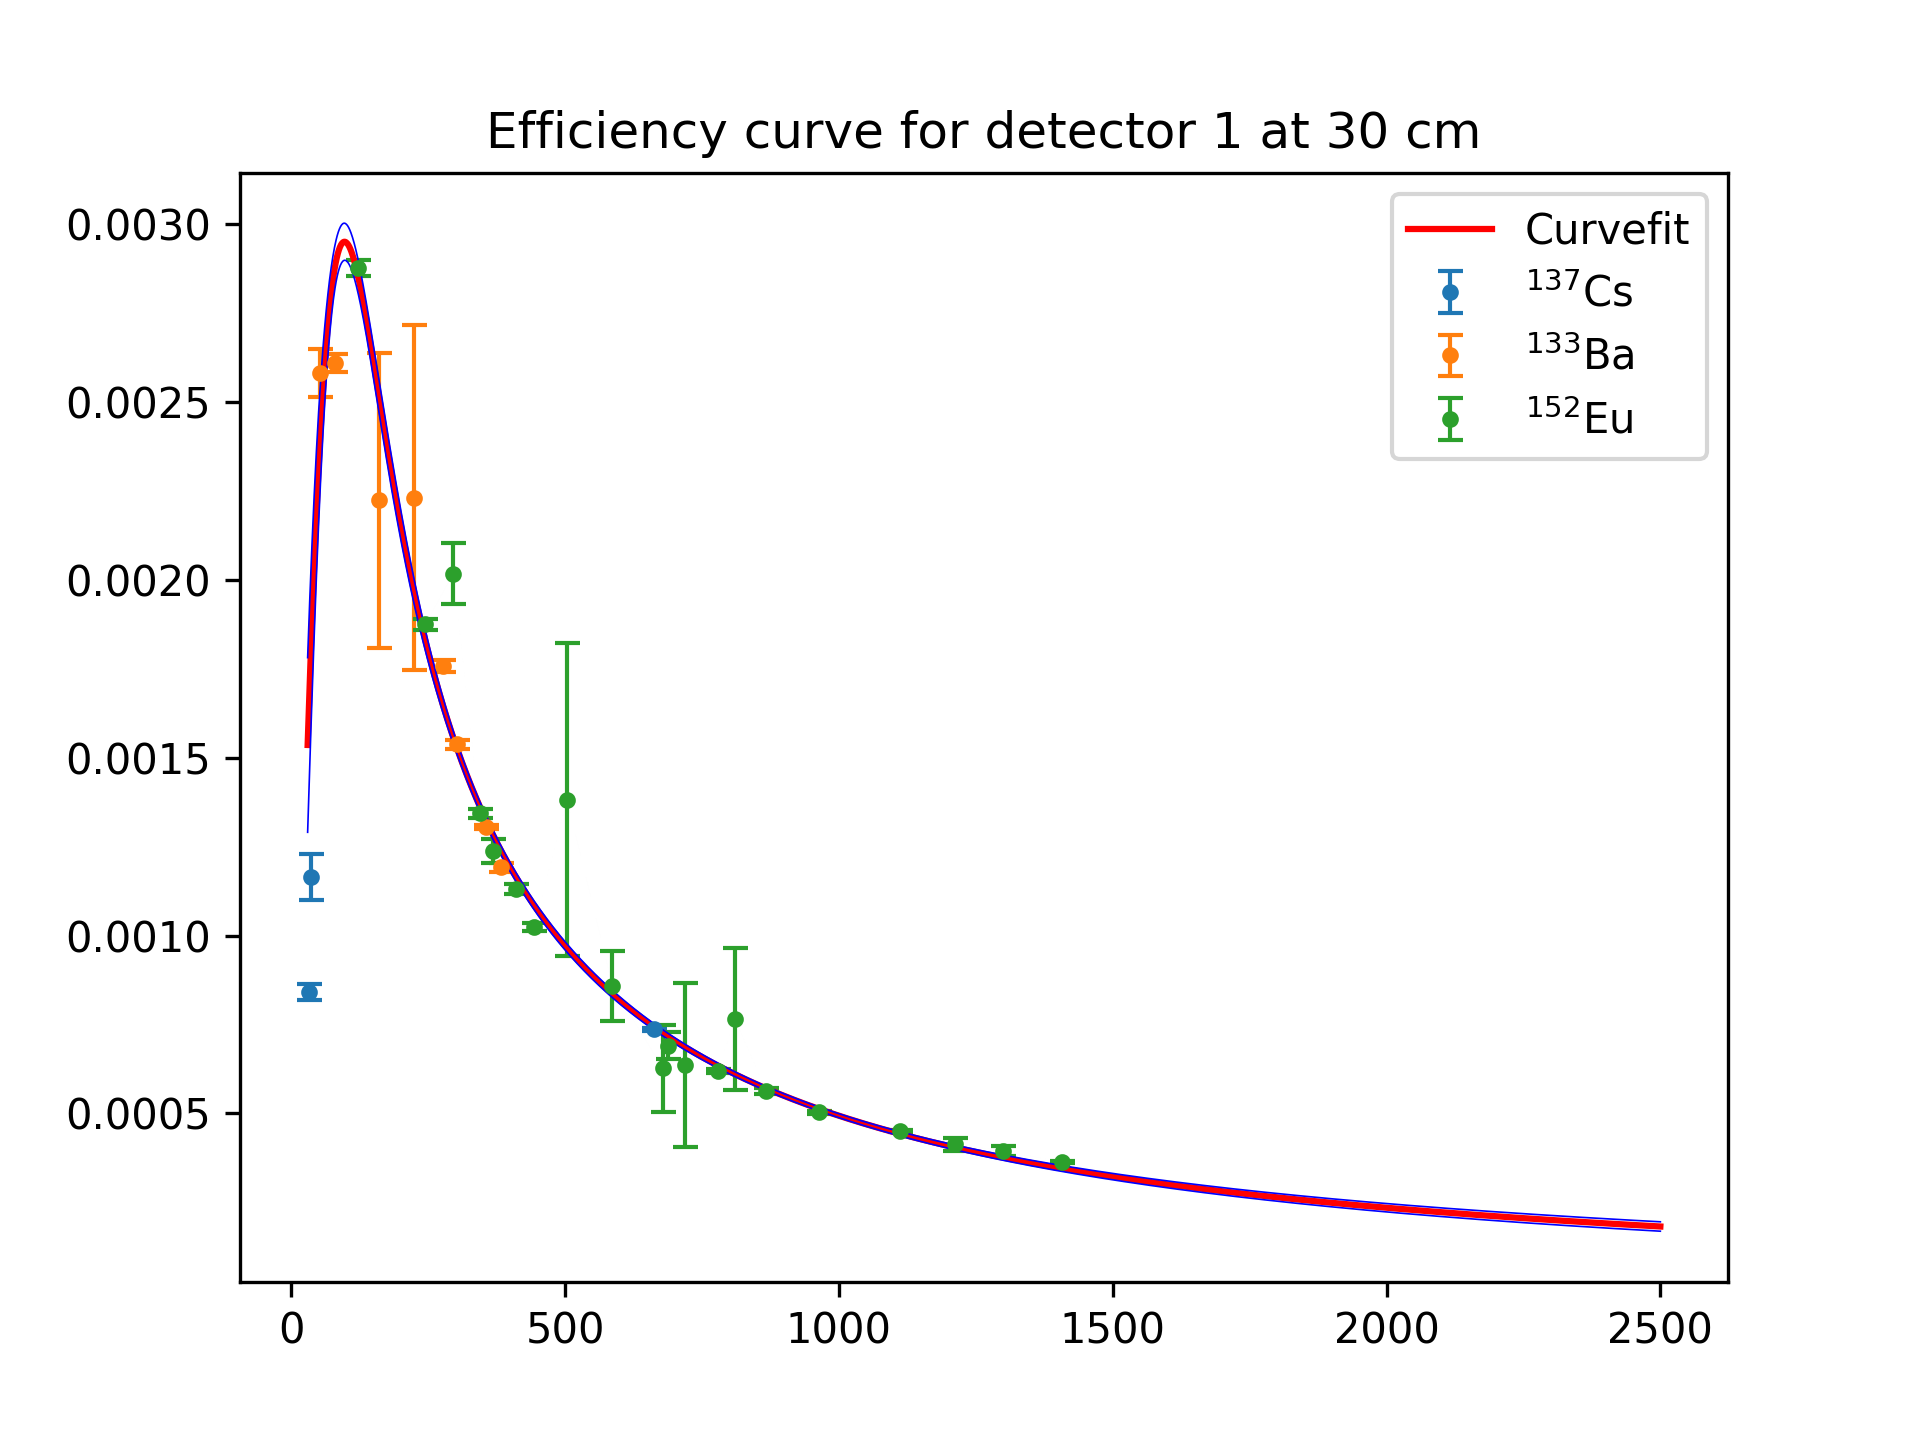
\includegraphics[width=12cm]{Experiment/new_det1_numb30cm.png} }}%
    
    \subfloat[]{{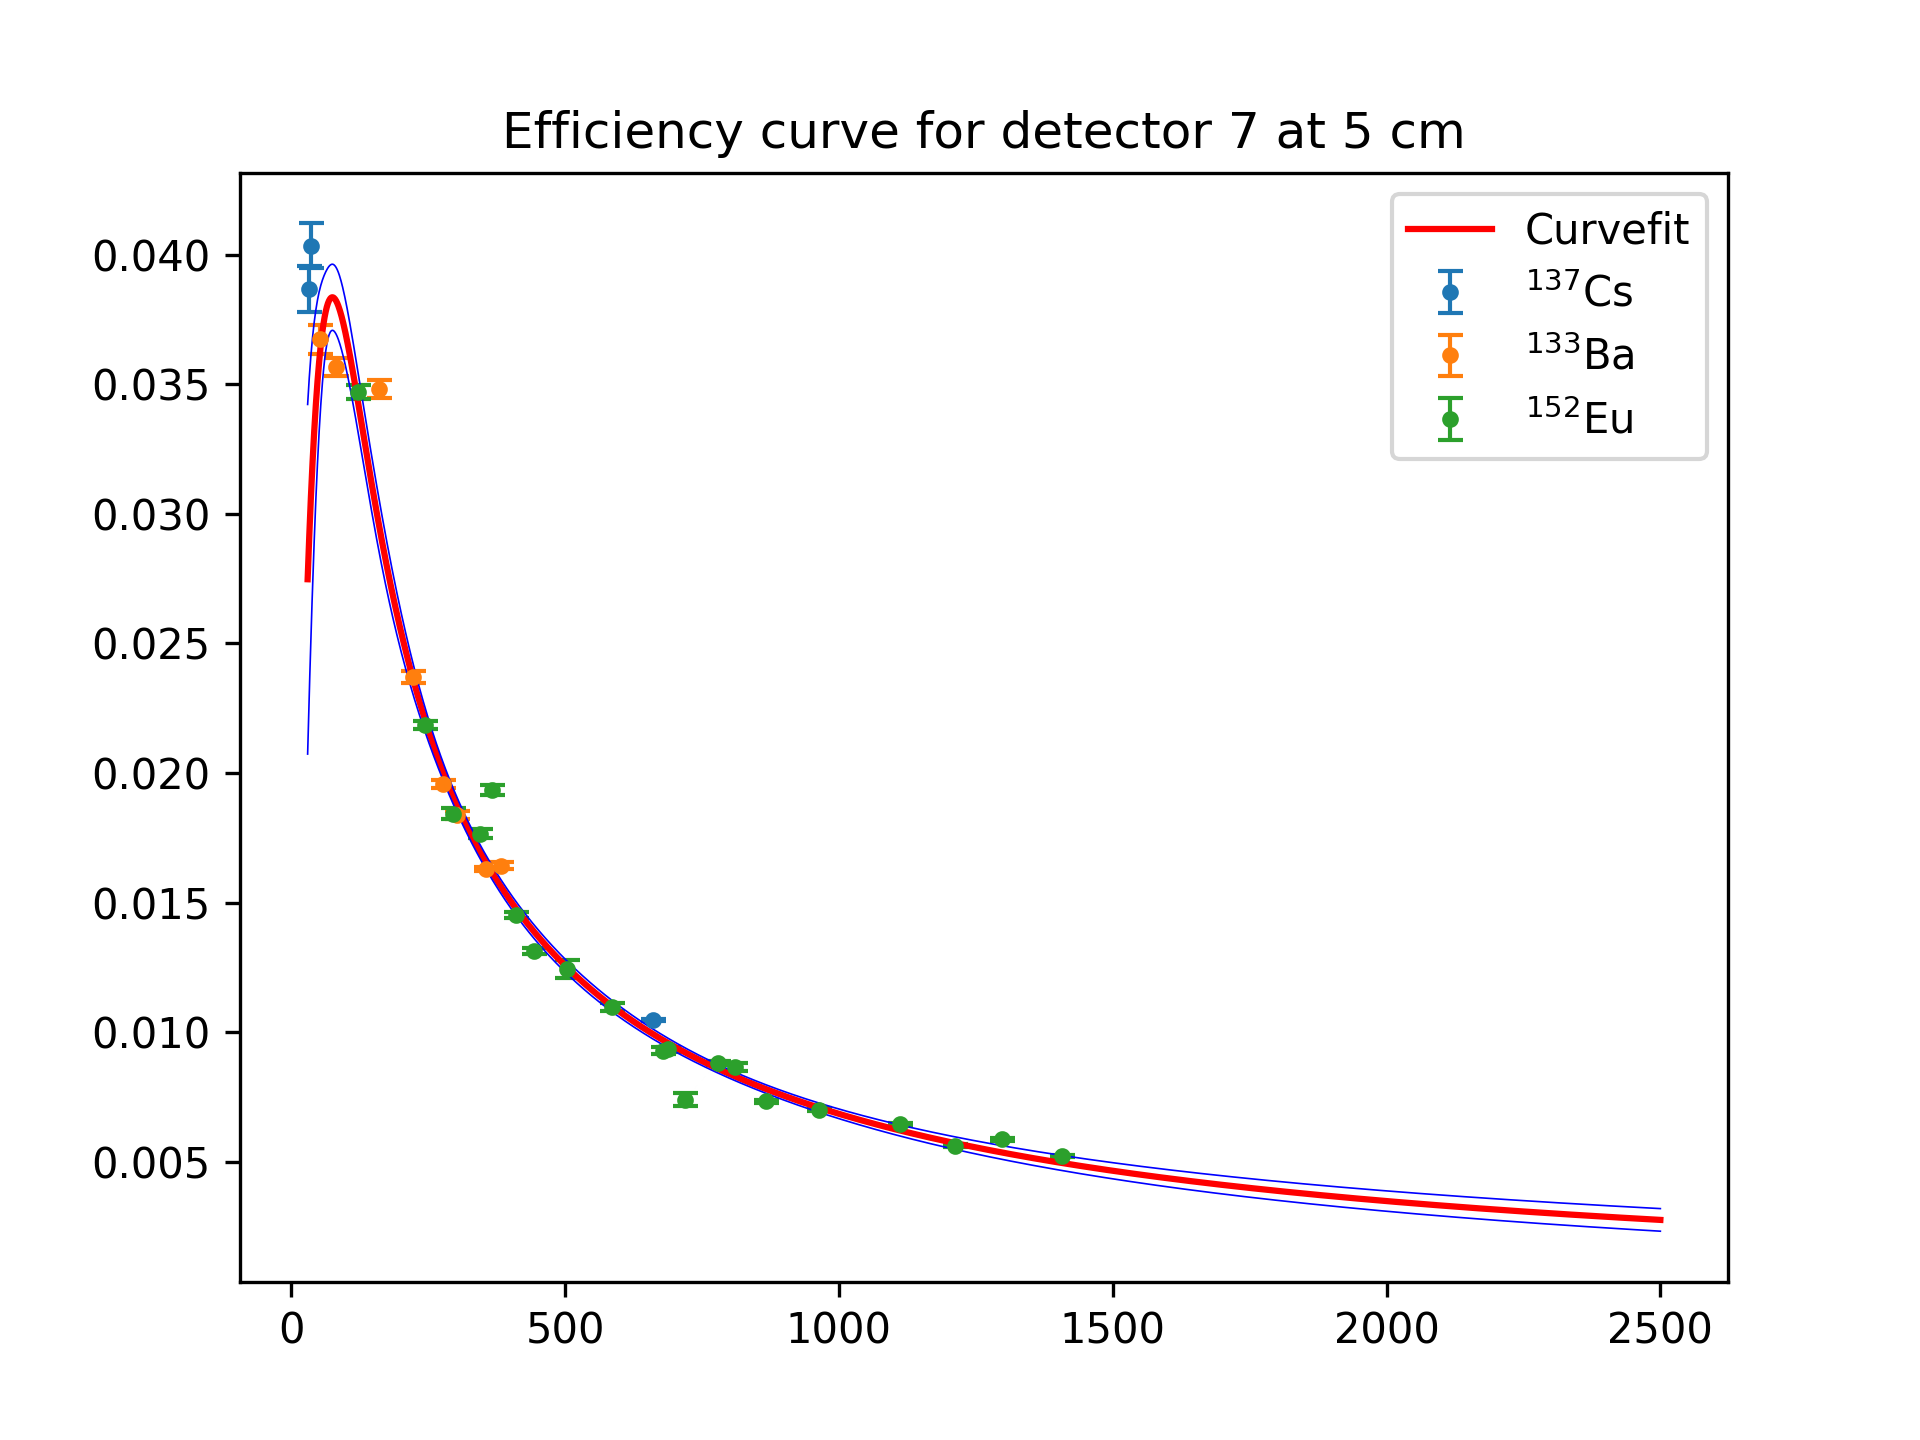
\includegraphics[width=12cm]{Experiment/new_det7_numb5cm.png} }}%
    \caption{Two examples of efficiency curves. \textbf{top}: The efficiencycurve of detector 1 at 30 cm which is located in cave 4C, and has a lower detector volume along with a different shape. \textbf{bottom:} The efficiency curve of detector 7 at 5 cm is located in a separate room and had led shielding. The geometry shape is better here!  }%
    \label{fig:efficiency_curves}%
\end{figure}




%\subsubsection{}

%The detectors were calibrated for efficiency,  peak shape and gamma-ray energy in the Gammaray-spectroscopy analyzation program Fitzpeaks. The calibration point sources $^{137}$Cs ($t_{1/2}=30.08$ years\cite{Browne2007}), $^{133}$Ba ($t_{1/2}=10.551$ years\cite{Khazov2011}) and $^{152}$Eu ($t_{1/2}=13.517$ years\cite{Martin2013}) were used with the gamma-lines listed in table \ref{table:calibration_gammas}. The calibration was done at various distances from the detector surface. The point sources can can be seen on figure \ref{fig:calsources}. The energy and peakshape calibration was done in FitzPeakz which is described in section \ref{subsec:fitz_calibration}. The efficiency calibration is described in section \ref{sec:efficiency_calibration}. \\ 



\section{The stacked target activation method} \label{sec:experiment}
The irradiation of the target stack took place on February 26th 2019, and the activated foils were counted on high purity germanium detectors for a total of 4 weeks after end of beam. \textcolor{red}{In addition to this experiment, two other experiments took place, irradiating strontium with deuterons and a deuteron breakup experiment}. The target stack was subject to a 33 MeV deuteron beam, which can be seen in figure \ref{fig:experiment_illustration} which from the beamintegrator read of 128.5 nA in beam current. The foils were ca. 25$\mu$m in thickness and measured approximately 25 by 25 mm in area. The beam was ca. 1 cm in diameter, so the beam was underfilling the targetfoils. \textcolor{red}{Why was it important that the beam was underfilled. On how was this related to the areal densities?}  \\

%The main motivation of this experiment was to measure production cross sections of the products produced after irradiation of a stack of thin iridium foils along with thin monitor foils nickel, copper and iron foils, with a 33 MeV incident deuteron beam, as shown in figure \ref{fig:experiment_illustration}. 
\begin{figure}
    \centering
    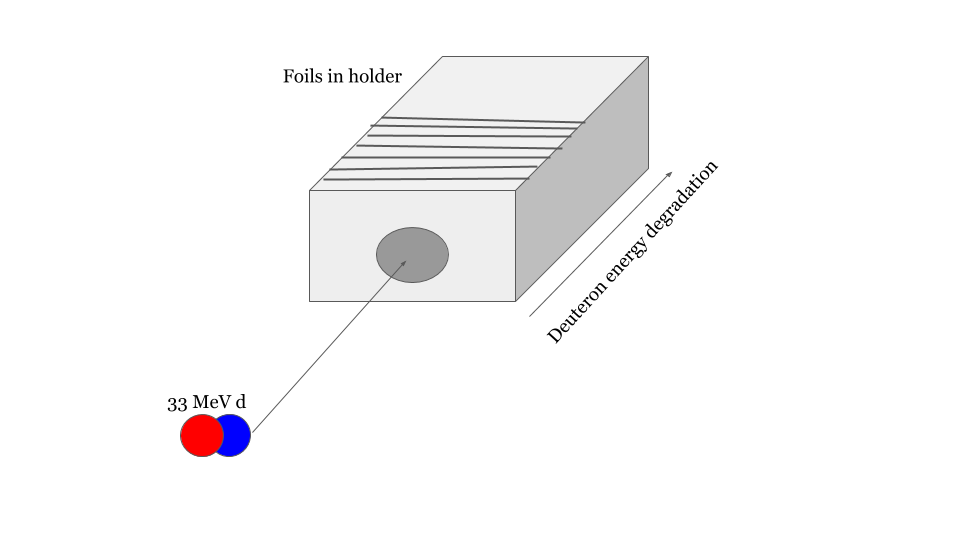
\includegraphics[width=0.7\textwidth]{Experiment/Illustration_beamOnTarget.png}
    \caption{The fundamental idea of the experiment where a stack of targets are placed in a target holder, and irradiated with accelerated 33 MeV deuterons. As the energy degrades through the beam stack, it is possible to have multiple cross section measurements at different energies.}
    \label{fig:experiment_illustration}
\end{figure}

\noindent 
The stacked-target method originates from Graves et. al. () irradiating a stack of thin iron, copper and aluminum foils with a 35-90 MeV protons beam \cite{Graves2016}. The method yields reaction cross section measurements at multiple energies for products which are observed in the foils with gamma-ray spectroscopy, as a stack of thin targets are exposed to a single incident charged particle beam which is degraded in the foils. Recent measurements conducted at Lawrence Berkeley's 88-Inch cyclotron have taken place over the past year using protonbeams for reactions on iron, copper and titanium from threshold to 55 MeV  \textcolor{red}{cite Fe-paper}%\footnote{https://www.researchgate.net/publication/336796889_Proton-induced_reactions_on_Fe_Cu_Ti_from_threshold_to_55_MeV}
and for reactions on niobium using 40-90 MeV protons\cite{Voyles2018c}. The induced activities in the foils can be measured and transferred into cross sections. For a thin foil, the beam degradation is small in comparison to thick targets, and the uncertainty in beam energy is thus small. In addition, the use of thin foils with a thickness of a few $\mu$m allows for low activation in each foil, which reduces dead time of the detector, along with lower dose to workers which is advantageous for isotope production and cross section measurement\cite{Qaim2017c}. \\

\noindent 
 The stack consisted of natural iridium (99.9\%), natural nickel (..), natural copper (..) and natural iron (..) from Goodfellow Corporation, Corapolis, PA 15108, USA. Deuteron-induced products from iridium was the main motivation behind this experiment, primarily because of the potential medically valuable $^{193m}$Pt-isomer, and the contribution of nuclear reaction data of the natural iridium (d,x) reactions. For the latter three targets, the well-characterized cross section reactions $^text{nat}$Fe(d,x)$^{56}$Co, $^\text{nat}$Ni(d,x)$^{61}$Cu$^{56,58}$Co and $^\text{nat}$Cu(d,x)$^{62,63,65}$Zn from the IAEA monitor database\cite{Hermanne2018a} were used to estimate the weighted average beam current throughout each compartment of foils. In addition, cross sections from deuteron induced products on these targets is a contribution to nuclear reaction data. The stack consisted of 10 nickel, 10 iridium, 10 copper and 3 iron foils, in which the order can be seen in table... In addition to the target foils, two 316 stainless steel foils were placed in the front and the back of the stack, and a 6061 aluminum alloy which works as a proton degrader along with a nickel neutron monitor foil \textcolor{red}{to stop broken up deuterons (protons+neutrons)}. Since the number of targets in the stack worked as a beam degrader, the need of additional energy degraders in the stack was not necessary. The stainless steel worked as a beam profile monitor, as the activated foils could be used to develop Gafcromic films (radiochromic films) which contains a dye changing color when exposed to ionizing radiation (wiki, radiochromic) which can be used to build confidence in the spatial beam profile in the front and in the back of the stack. The full order of the stack can be viewed in table \ref{table:foil_characterization}. The stack design was decided upon the energy-degradation  of the stack with a package called NPAT's (nuclear ....) Ziegler simulation, which bases the stopping power on Anderson \& Ziegler stoppingpower formalism \cite{A\&Z, John}, so that the beam was not stopped in the target stack.  

\noindent 
%From equation \ref{eq:activity_eob}, the cross section as a function of energy is 

%\begin{equation} \label{eq:experimental_CS}
%    \sigma(E)=\frac{A_0}{N_T \Phi (1-e^{-\lambda \Delta t_\text{irr}})}
%\end{equation}

\noindent 
%where E is the average energy across the foil (MeV), $A_0$ is the end of beam activity (Bq), $N_T$ is the number of target nuclei, $\Phi$ is the beam current (nA), $\lambda$ is the decay constant of the nucleus ($s^{-1}$) and $\Delta t_\text{irr}$ is the irradiation length (s). 

\noindent 
%Equation \ref{eq:cross_section_equation} is the equation which is used in the calculation of the cross sections. In order to calculate the cross section of a product, end of beam activity, number of target nuclei and beam current must be found, where for the end of beam activity, the detector efficiency need to be estimated. The number of target nuclei was estimated through characterization of the foils. $A_0$ was estimated using equation \ref{eq:Final_Expression_A0}, which depends on the efficiency calibration of the detectors as a function of gamma-ray energy, the number of counts registered and the intensity of the gamma-rays emitted by the source, the decay constant of the source and the delay time. Some of the nickel, copper and iron deuteron-induced cross section are well-established, and can  be used to determine the beam current throughout the stack. 



%The end of beam activity goes into the equation, which is given in equation \ref{eq:Final_Expression_A}. The activity from spectra measured at different delay times after end of beam can be found, with respect to number of counts, efficiency of detector, intensity of gamma-rays, the decay constant of the nucleus $\lambda$ and the counting time $\Delta t_c$. As we know that radioactive decay curves follows equation \ref{eq:ndecay_chains}, and dependent on how many step the decaychain consists of, the end of beam activity can be estimated by extrapolating backwards in time with a curve fit. \\

%\noindent 


\subsection{Characterization of the target foils} \label{subsec:target_design}

%\textcolor{red}{why was the order what it was??}
%In this experiment, the target stack was composed of of ten natural iridium foils (99.9\%) foils, along with ten natural nickel foils (..\%), ten natural copper foils (..\%) and three natural iron foils (..\%) (from Goodfellow Corporation, Corapolis, PA 15108, USA) serving as monitor foils. Along with two stainless steel foils in the front and the back of the stack, a proton degrader (a 6061 aluminum alloy), and an extra nickel neutron monitor foil was used to obtain production cross sections at multiple energies, using one incident deuteron beam. The full order of the stack and the characterization of each foil can be seen in table \ref{table:foil_characterization}. \\

\noindent 
The iridium foils were bought in 25 by 25 mm squares, and the copper, iron and nickel foils were cut into approximately 25 by 25 mm squares, where each foil was cut from the same \textcolor{red}{sample}. The length of each foil along each side and the thickness was measured with a caliper (Mitutoyo Absoule Digimatic) and a gauge caliper (Mitutoyo IP65 Coolant Proof) respectively. An analytical balance weight (Mettler Toledo) was used to measure the mass of each foil which was prewashed with isopropanol to clear the foils from surface contamination. Each unit was measured four times, and the values listed in table \ref{table:foil_characterization} are the averaged measurements. The mass density was calculated for each foil which was calculated using the average mass of each foil, divided by the averaged area. The uncertainty in the areal density was calculated as the standard deviation of the data described in equation \ref{eq:standard_dev}. The areal densities were later in the analysis converted to number of nuclei per cm$^2$, which was done numerically multiplying the mass density with Avogadro's number, and dividing by the mol-mass of the target atoms. The measured thicknesses were not used in the analysis, but was a confirmation that the foils were ca. 25 $\mu$m in thickness. The measured values varied from 24.3$\mu$m (Ir03) to 34.8 $\mu$m (Cu02), which were within accepted values. 

%The length and mass were used to measure the mass density. The thickness was not used in the
%calculation of the mass density, but was a good indication that the foil thicknesses were consistent.
%\textcolor{red}{For underfilled beams, the mass density of the foil is used to find the number of nuclei per cm$^2$, by using the area of each foil.} The mass density was calculated using the mass of each foil divided by the area
%\begin{equation}
%    \rho \Delta r = \frac{m}{A}
%\end{equation}

%\noindent 
%The uncertainty in each parameter was calculated using the standard deviation (equation \ref{eq:standard_dev}) of the four measurements per unit, and the total uncertainty was calculated using the approximation of uncorrelated variables used in equation \ref{eq:uncertainty_simplification}. The conversion from mg per cm$^2$ to nuclei per cm$^2$ was done numerically, by multiplying the mass density with Avogadro's number $N_A$ and dividing by the mol-mass of the target atoms. \\

\noindent 
After the characterization, each foil was mounted on ca. 1.6 mm thick plastic frames over a hollow center and attached with \textcolor{red}{3M 5413-Series Kapton polyimide film??} tape along the edges. From previous experiments, the Kapton tape has been used to seal the foils into airtight pockets for foil containment, but has appeared to have an impact on the proton stopping power \cite{https://www.researchgate.net/publication/336796889_Proton-induced_reactions_on_Fe_Cu_Ti_from_threshold_to_55_MeV}. There it was not placed near where the deuteron beam would activate the foil. The target frames can be seen in figure \ref{fig:targets_on_frame}. For irradiation, the foils were placed in a target holder which was a 6061 aluminum allow with a hollow center in the front for the beamline to pass through. A hollow spring was used to keep the foils stable during the irradiation. The target holder can be seen in figure \ref{fig:targetstack} (left).    

\begin{figure}
    \centering
    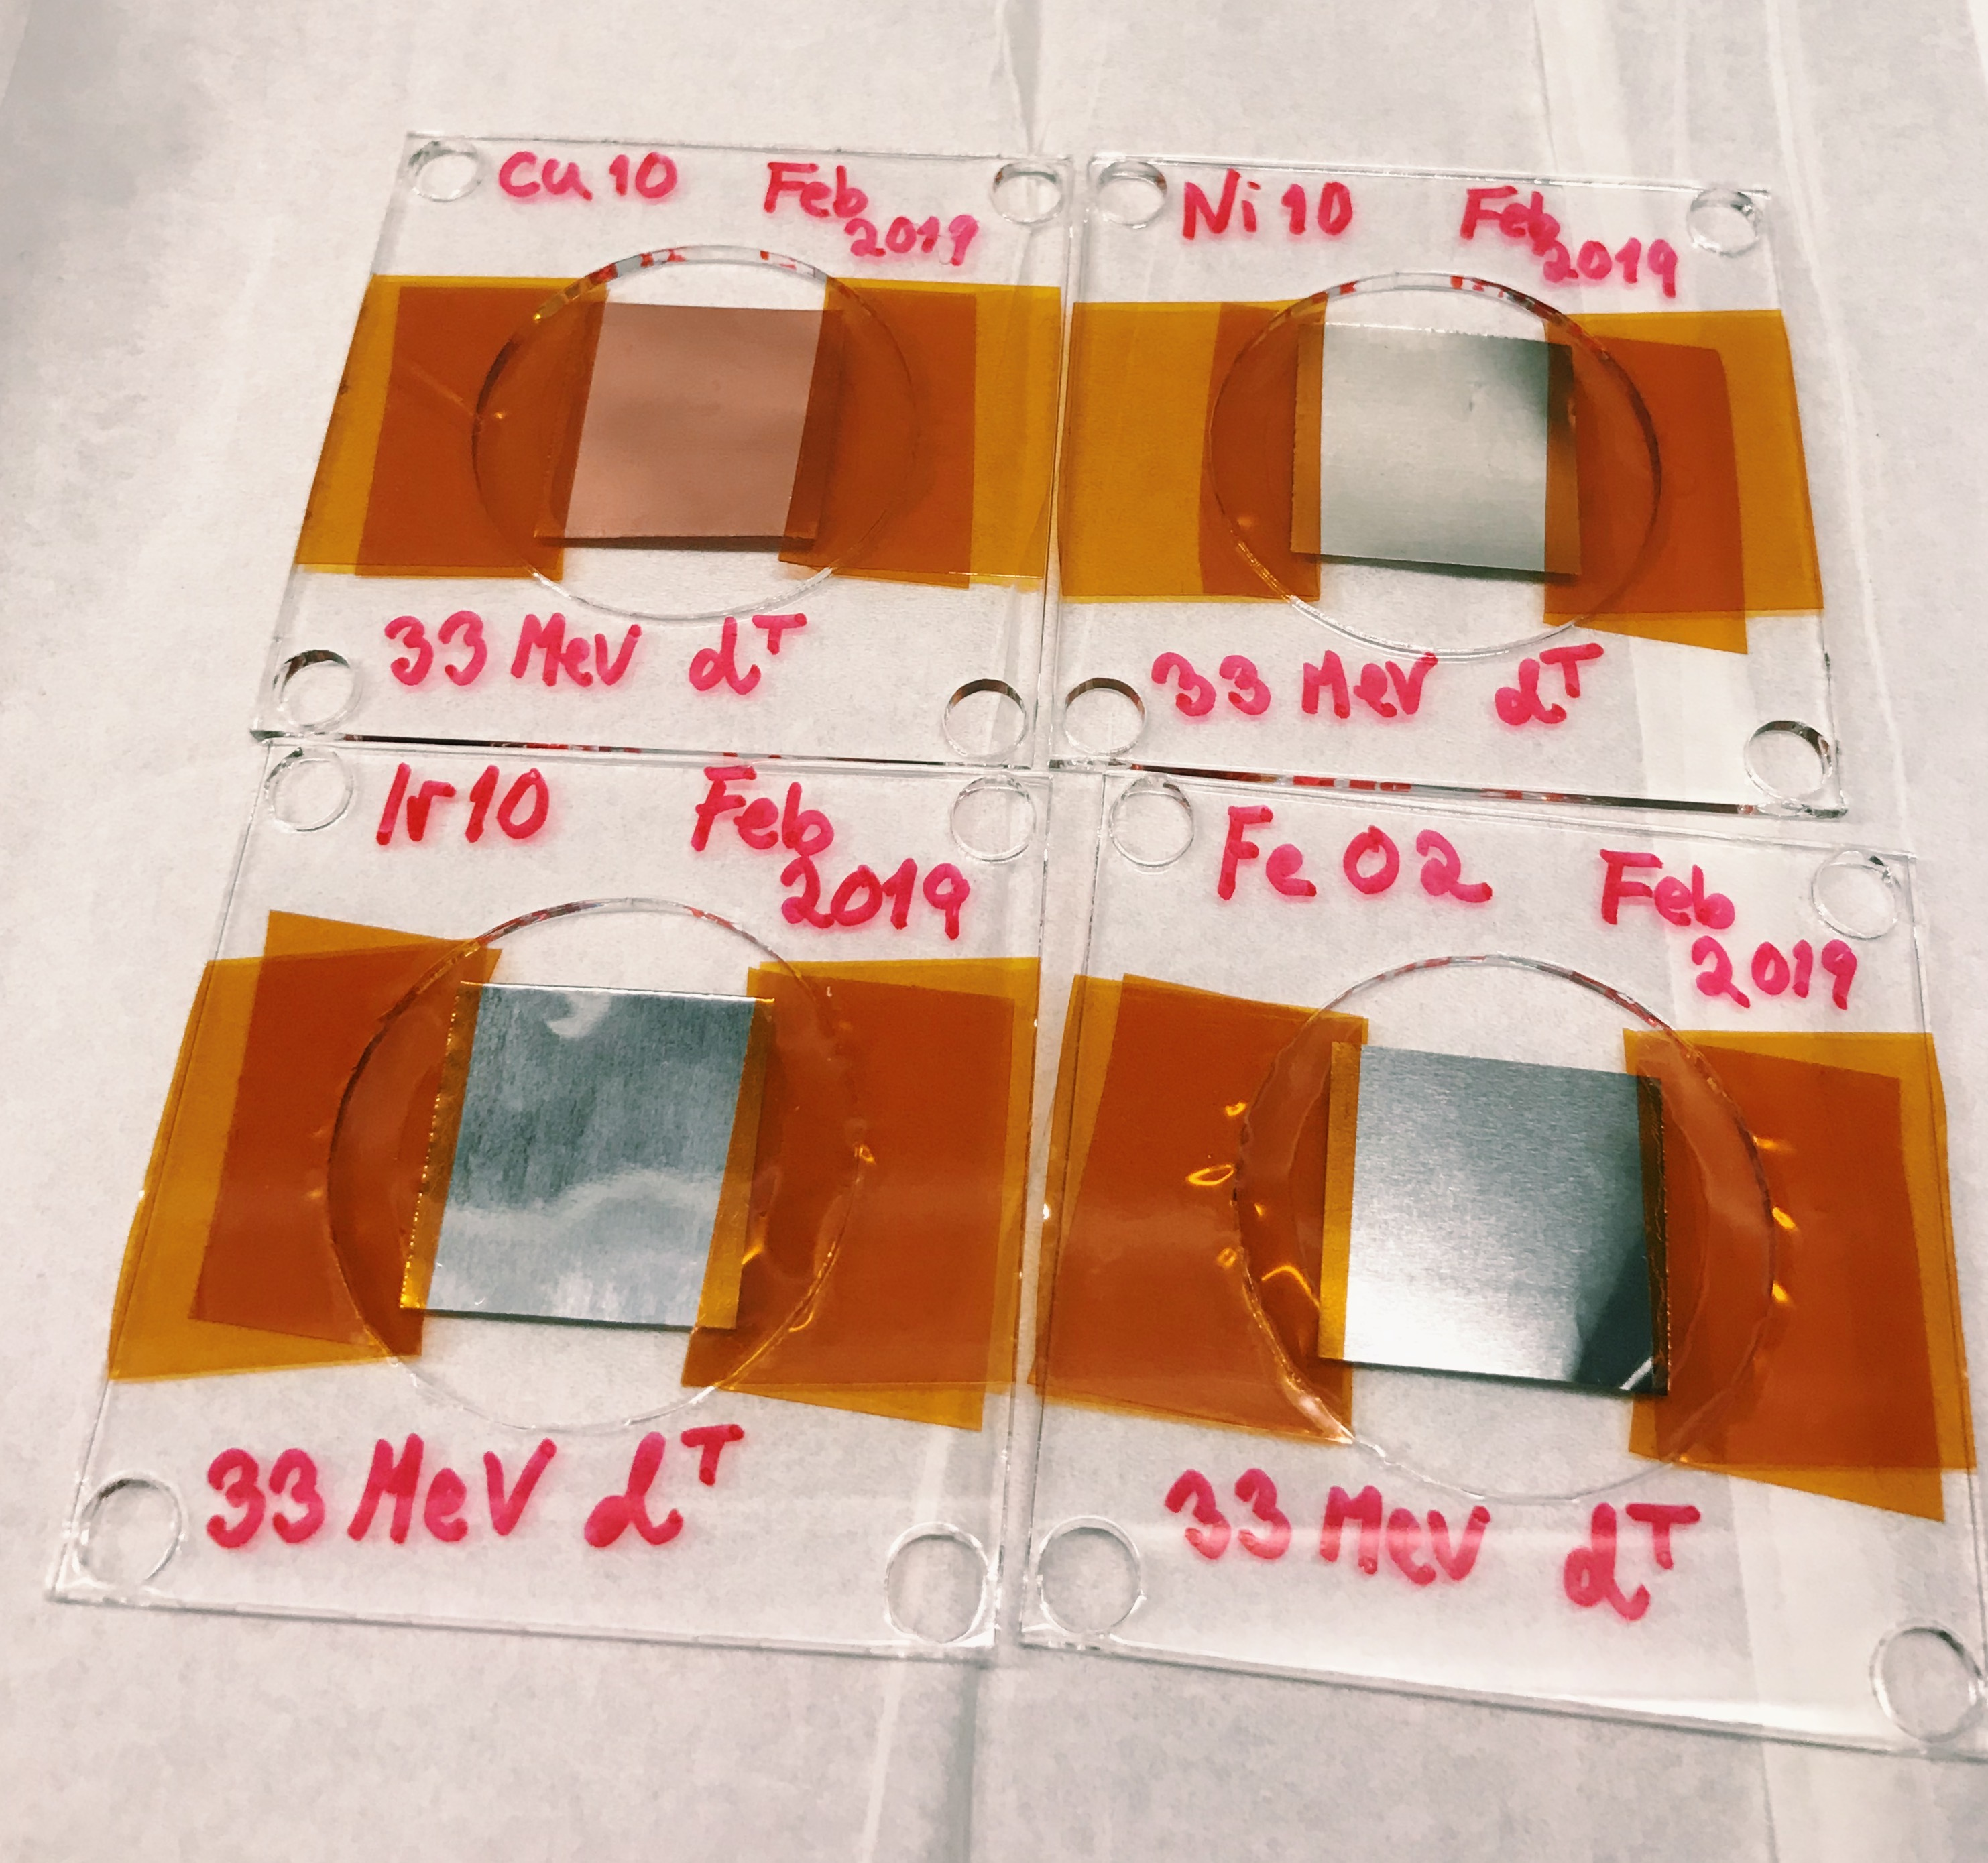
\includegraphics[width=0.5\textwidth]{Experiment/targets_on_frame.JPG}
    \caption{The figure shows the four different targets mounted on plastic frames with capton tape attached along the edges of the foils.}
    \label{fig:targets_on_frame}
\end{figure}


\begin{table}[h!]
%\centering
\caption{Characterization of each foil, along with calculated mass density. Each length is measured in mm, and mass in grams. *: measured from previous experiments}
\label{table:foil_characterization}
\small
\begin{tabular}{lllllll}
\makecell{\textbf{Foil}} & \makecell{Length1 (mm)}  &  \makecell{Length2 (mm)} & \makecell{Thickness (mm)} & \makecell{Mass (g)} & \makecell{\textbf{Mass density (mg/cm$^2$)}} \\ 
\hline
\makecell{SS1} & \makecell{} & \makecell{} & \makecell{} & \makecell{} & \makecell{100.199^*} \\
\hline
\makecell{Ni01} & \makecell{25.228} & \makecell{25.293} & \makecell{0.0285} & \makecell{0.1453} & \makecell{22.772 $\pm$ 0.138} \\
\makecell{Ir01} & \makecell{24.943} & \makecell{24.968} & \makecell{0.0295} & \makecell{0.3436} & \makecell{55.174 $\pm$ 0.053} \\
\makecell{Cu01} & \makecell{25.553} & \makecell{24.883} & \makecell{0.0341} & \makecell{0.1420} & \makecell{22.338 $\pm$ 0.048} \\
\makecell{Fe01} & \makecell{24.400} & \makecell{26.068} & \makecell{0.0278} & \makecell{0.1274} & \makecell{20.030 $\pm$ 0.110} \\
\hline
\makecell{Ni02} & \makecell{25.288} & \makecell{25.428} & \makecell{0.0295} & \makecell{0.1487} & \makecell{23.118 $\pm$ 0.096} \\
\makecell{Ir02} & \makecell{24.923} & \makecell{25.005} & \makecell{0.0278} & \makecell{0.3465} & \makecell{55.601 $\pm$ 0.238} \\
\makecell{Cu02} & \makecell{25.443} & \makecell{25.550} & \makecell{0.0348} & \makecell{0.1451} & \makecell{22.325 $\pm$ 0.028} \\
\makecell{Fe02} & \makecell{25.525} & \makecell{23.800} & \makecell{0.0274} & \makecell{0.1216} & \makecell{20.017 $\pm$ 0.034} \\
\hline
\makecell{Ni03} & \makecell{25.295} & \makecell{25.210} & \makecell{0.0270} & \makecell{0.1425} & \makecell{22.338 $\pm$ 0.066} \\
\makecell{Ir03} & \makecell{24.885} & \makecell{24.983} & \makecell{0.0243} & \makecell{0.3459} & \makecell{55.643 $\pm$ 0.121} \\
\makecell{Cu03} & \makecell{25.560} & \makecell{25.508} & \makecell{0.0343} & \makecell{0.1455} & \makecell{22.313 $\pm$ 0.043} \\
\makecell{Fe03} & \makecell{26.113} & \makecell{25.235} & \makecell{0.0310} & \makecell{0.1315} & \makecell{19.948 $\pm$ 0.114} \\
\hline
\makecell{Ni04} & \makecell{25.303} & \makecell{24.888} & \makecell{0.0273} & \makecell{0.1304} & \makecell{20.704 $\pm$ 0.068} \\
\makecell{Ir04} & \makecell{24.960} & \makecell{24.833} & \makecell{0.0261} & \makecell{0.3471} & \makecell{56.000 $\pm$ 0.109} \\
\makecell{Cu04} & \makecell{25.153} & \makecell{25.603} & \makecell{0.0333} & \makecell{0.1435} & \makecell{22.284 $\pm$ 0.027} \\
\hline
\makecell{Ni05} & \makecell{25.325} & \makecell{25.495} & \makecell{0.0263} & \makecell{0.1406} & \makecell{21.768 $\pm$ 0.045} \\
\makecell{Ir05} & \makecell{24.948} & \makecell{24.958} & \makecell{0.0256} & \makecell{0.3435} & \makecell{55.161 $\pm$ 0.081} \\
\makecell{Cu05} & \makecell{25.213} & \makecell{25.573} & \makecell{0.0334} & \makecell{0.1447} & \makecell{22.443 $\pm$ 0.028} \\
\hline
\makecell{Ni06} & \makecell{25.530} & \makecell{25.195} & \makecell{0.0285} & \makecell{0.1471} & \makecell{22.861 $\pm$ 0.123} \\
\makecell{Ir06} & \makecell{24.760} & \makecell{24.960} & 
\makecell{0.0240} & \makecell{0.3444} & \makecell{55.731 $\pm$ 0.088} \\
\makecell{Cu06} & \makecell{25.343} & \makecell{25.513} & \makecell{0.0340} & \makecell{0.1448} & \makecell{22.396 $\pm$ 0.012} \\
\hline
\makecell{Ni07} & \makecell{25.338} & \makecell{25.278} & \makecell{0.0268} & \makecell{0.1479} & \makecell{23.092 $\pm$ 0.078} \\
\makecell{Ir07} & \makecell{24.955} & \makecell{25.008} & \makecell{0.0278} & \makecell{0.3538} & \makecell{56.685 $\pm$ 0.085} \\
\makecell{Cu07} & \makecell{25.625} & \makecell{25.248} & \makecell{0.0326} & \makecell{0.1444} & \makecell{22.320 $\pm$ 0.014} \\
\hline
\makecell{Ni08} & \makecell{25.205} & \makecell{24.950} & \makecell{0.0256} & \makecell{0.1409} & \makecell{22.409 $\pm$ 0.124} \\
\makecell{Ir08} & \makecell{24.723} & \makecell{24.985} & \makecell{0.0281} & \makecell{0.3585} & \makecell{58.030 $\pm$ 0.130} \\
\makecell{Cu08} & \makecell{25.370} & \makecell{24.885} & \makecell{0.0333} & \makecell{0.1414} & \makecell{22.401 $\pm$ 0.033} \\
\hline
\makecell{Ni09} & \makecell{25.220} & \makecell{25.378} & \makecell{0.0257} & \makecell{0.1392} & \makecell{21.741 $\pm$ 0.073} \\
\makecell{Ir09} & \makecell{24.670} & \makecell{24.993} & \makecell{0.0273} & \makecell{0.3494} & \makecell{56.669 $\pm$ 0.043} \\
\makecell{Cu09} & \makecell{25.390} & \makecell{26.455} & \makecell{0.0331} & \makecell{0.1506} & \makecell{22.425 $\pm$ 0.041} \\
\hline
\makecell{Ni10} & \makecell{25.285} & \makecell{24.405} & \makecell{0.0271} & \makecell{0.1425} & \makecell{23.093 $\pm$ 0.024} \\
\makecell{Ir10} & \makecell{24.973} & \makecell{24.980} & \makecell{0.0270} & \makecell{0.3435} & \makecell{55.065 $\pm$ 0.055} \\
\makecell{Cu10} & \makecell{25.470} & \makecell{25.338} & \makecell{0.0355} & \makecell{0.1440} & \makecell{22.314 $\pm$ 0.047} \\
\hline


\hline
\makecell{SS2} & \makecell{} & \makecell{} & \makecell{} & \makecell{} & \makecell{100.865^*} \\
\makecell{P-degrader} & \makecell{} & \makecell{} & \makecell{} & \makecell{} & \makecell{1900.0^*} \\
\makecell{Ni neutron monitor} & \makecell{} & \makecell{} & \makecell{} & \makecell{} & \makecell{\textbf{?}} \\
\hline
\end{tabular}
\end{table}


\subsubsection{The tuning the beam}
Before irradiation, the deuteron beam was tuned to be ca. 1 cm in diameter. In addition, the experiments taking place simultaneously demanded a precise position of the beamspot since the targets were small in size. The beam spot was first visualized using a ca. 2.5 cm thick borosilicate glass, painted with a mixture of phosphor powder and vacuum grease (so that the paint does not evaporate as the tube was pumped down to vacuum). When ionizing radiation strikes the phosphor, the phosphor is excited and emits light in the de-excitation, called phosphorescence.  The glass was placed on the end of the beam tube. With a camera placed in cave 0, from the control room, the beam spot could be visualized, and could be steered to be centered and ca. 1 cm in diameter. The beamspot can be visalized in figure \ref{fig:tuning_phosphor+camera} (left), and the borosilicate glass placed on the end of the beam tube can be seen in figure \ref{fig:tuning_phosphor+camera} (right). Secondly, the beam had to be constant over the target stack, ie. not diverge or converge. Gafchromic films were placed in the front and the back of the target holder, separated by the spring. The films were exposed for a brief second, and the blue spot on the developed film was evaluated. This was done until the beamspot was good both in the front and in the back of the stack. The Gafchromic films after direct exposure can be seen in figure \ref{fig:tuning_gafchromic} in the target holder.  \\

\begin{figure}%
    \centering
    \subfloat[]{{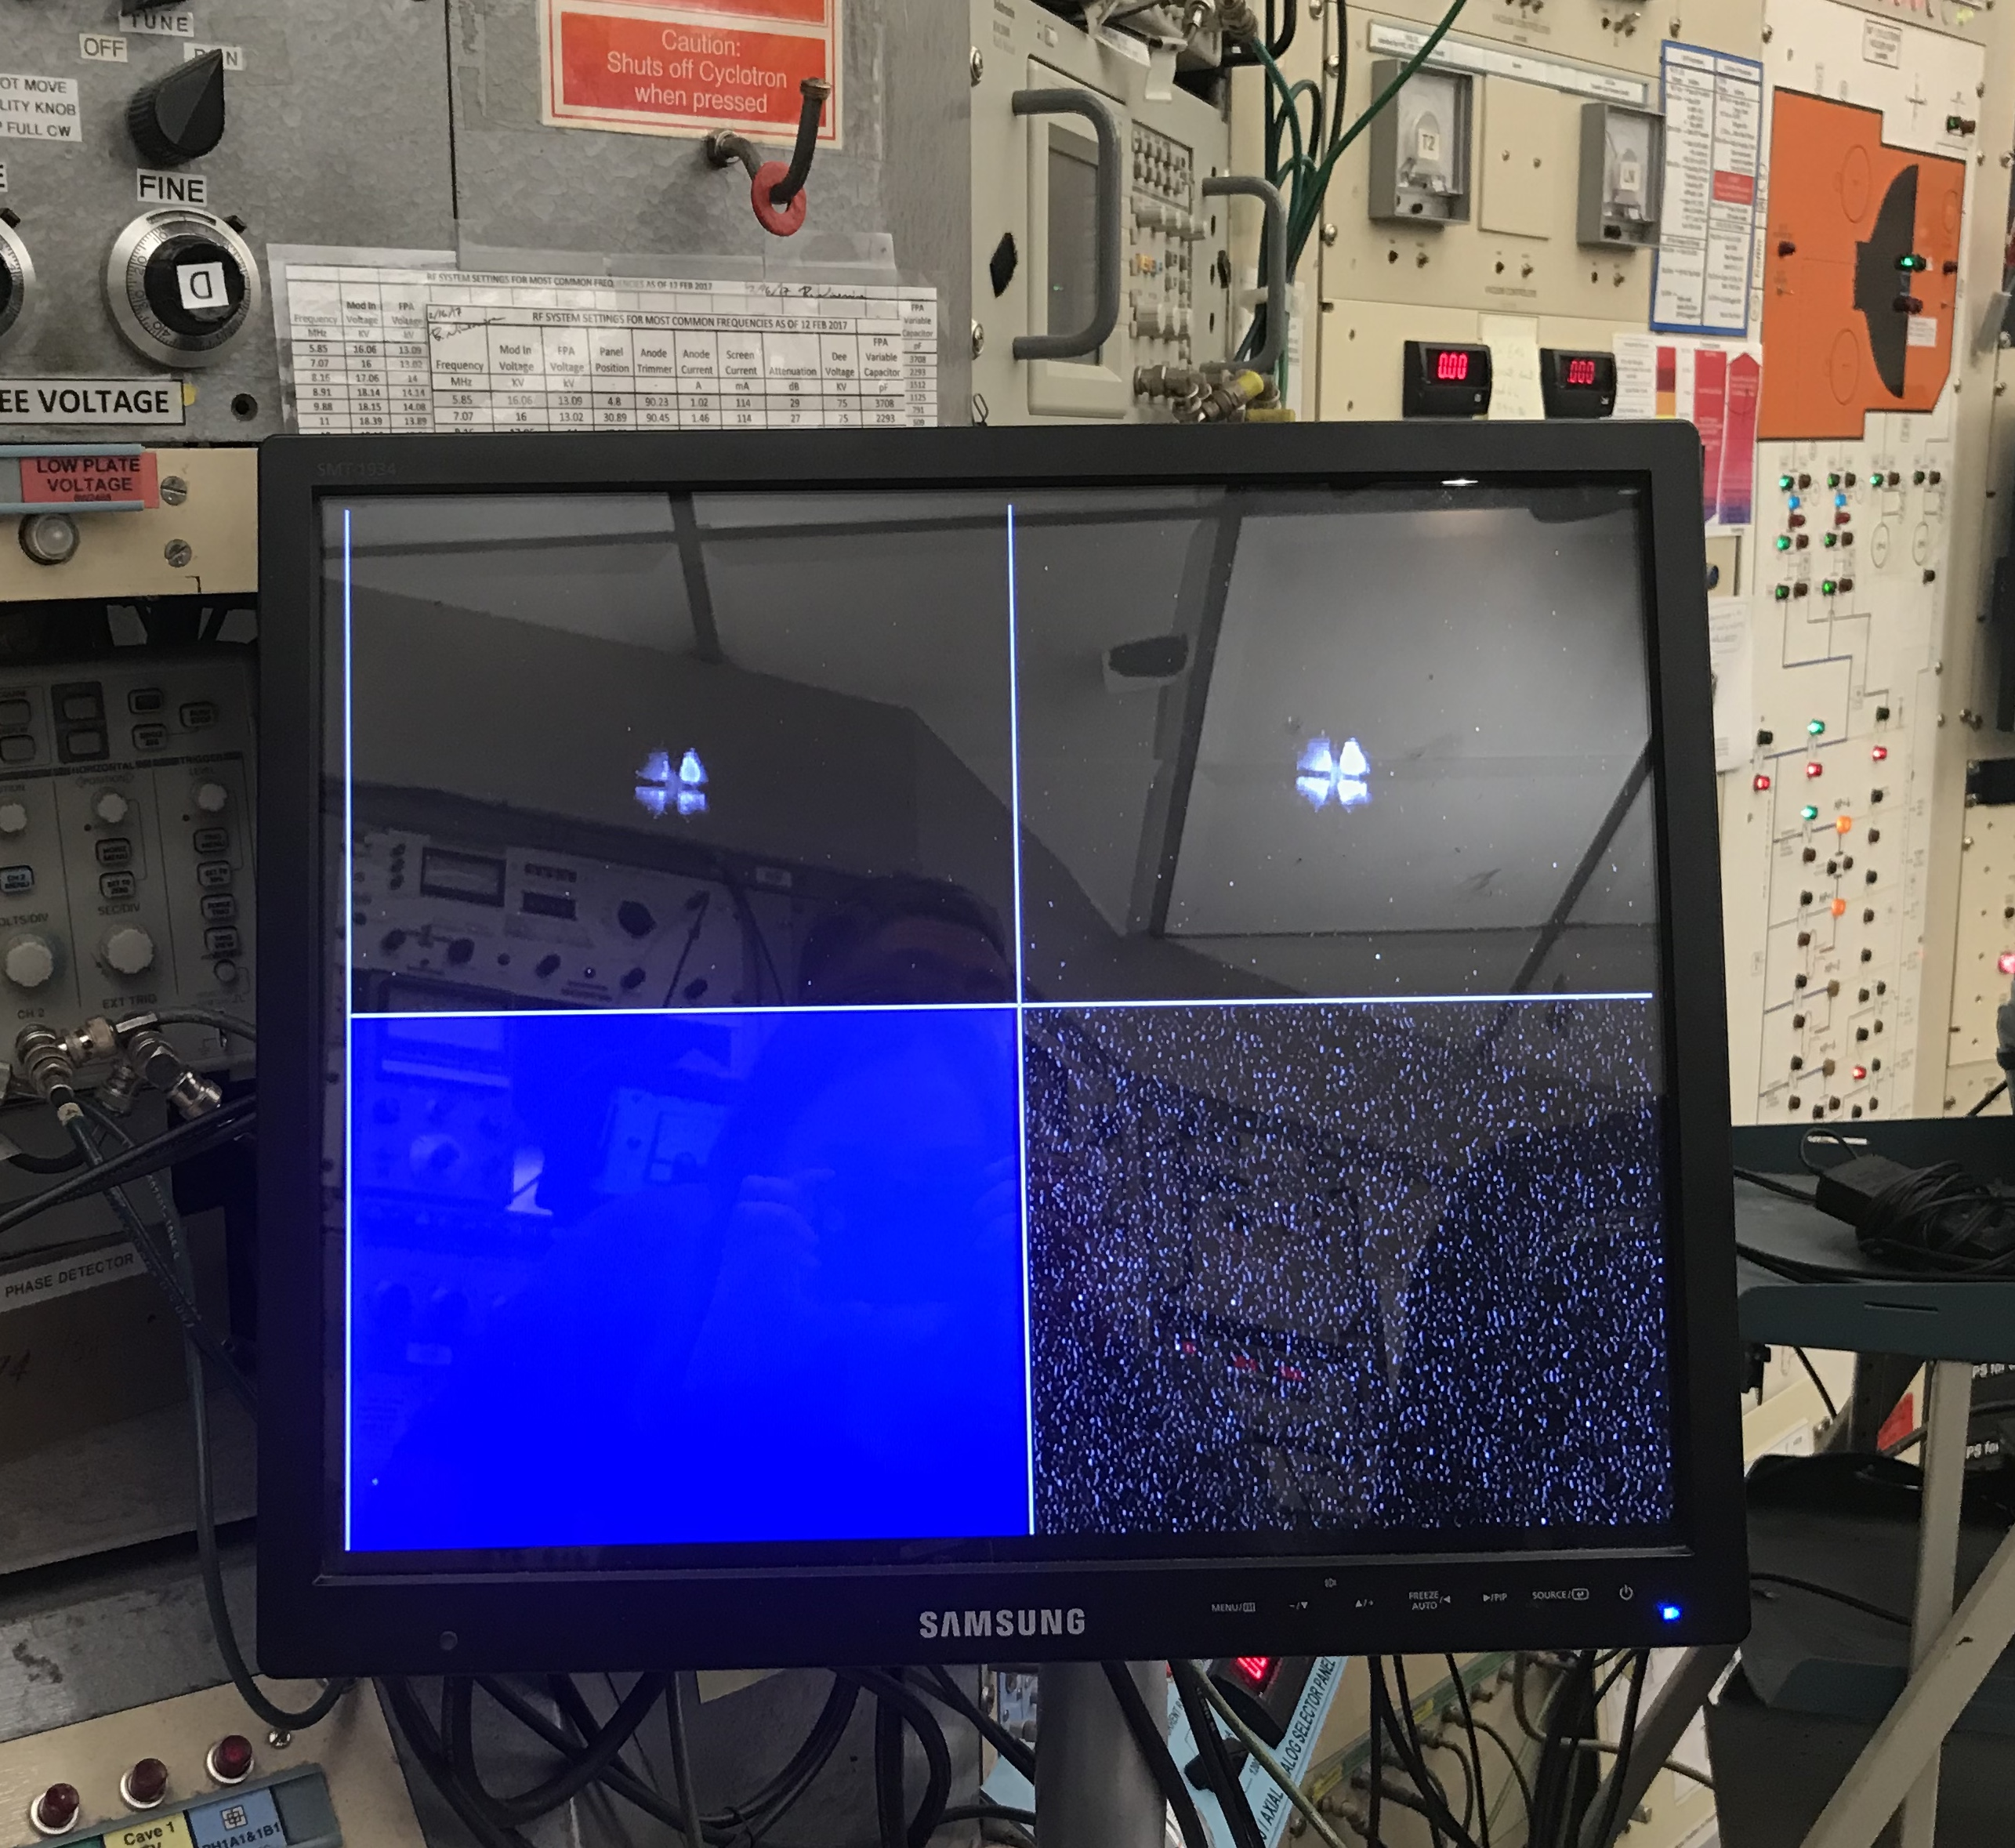
\includegraphics[width=6.6cm]{Experiment/beamspot_visualization.jpg} }}%
    \subfloat[]{{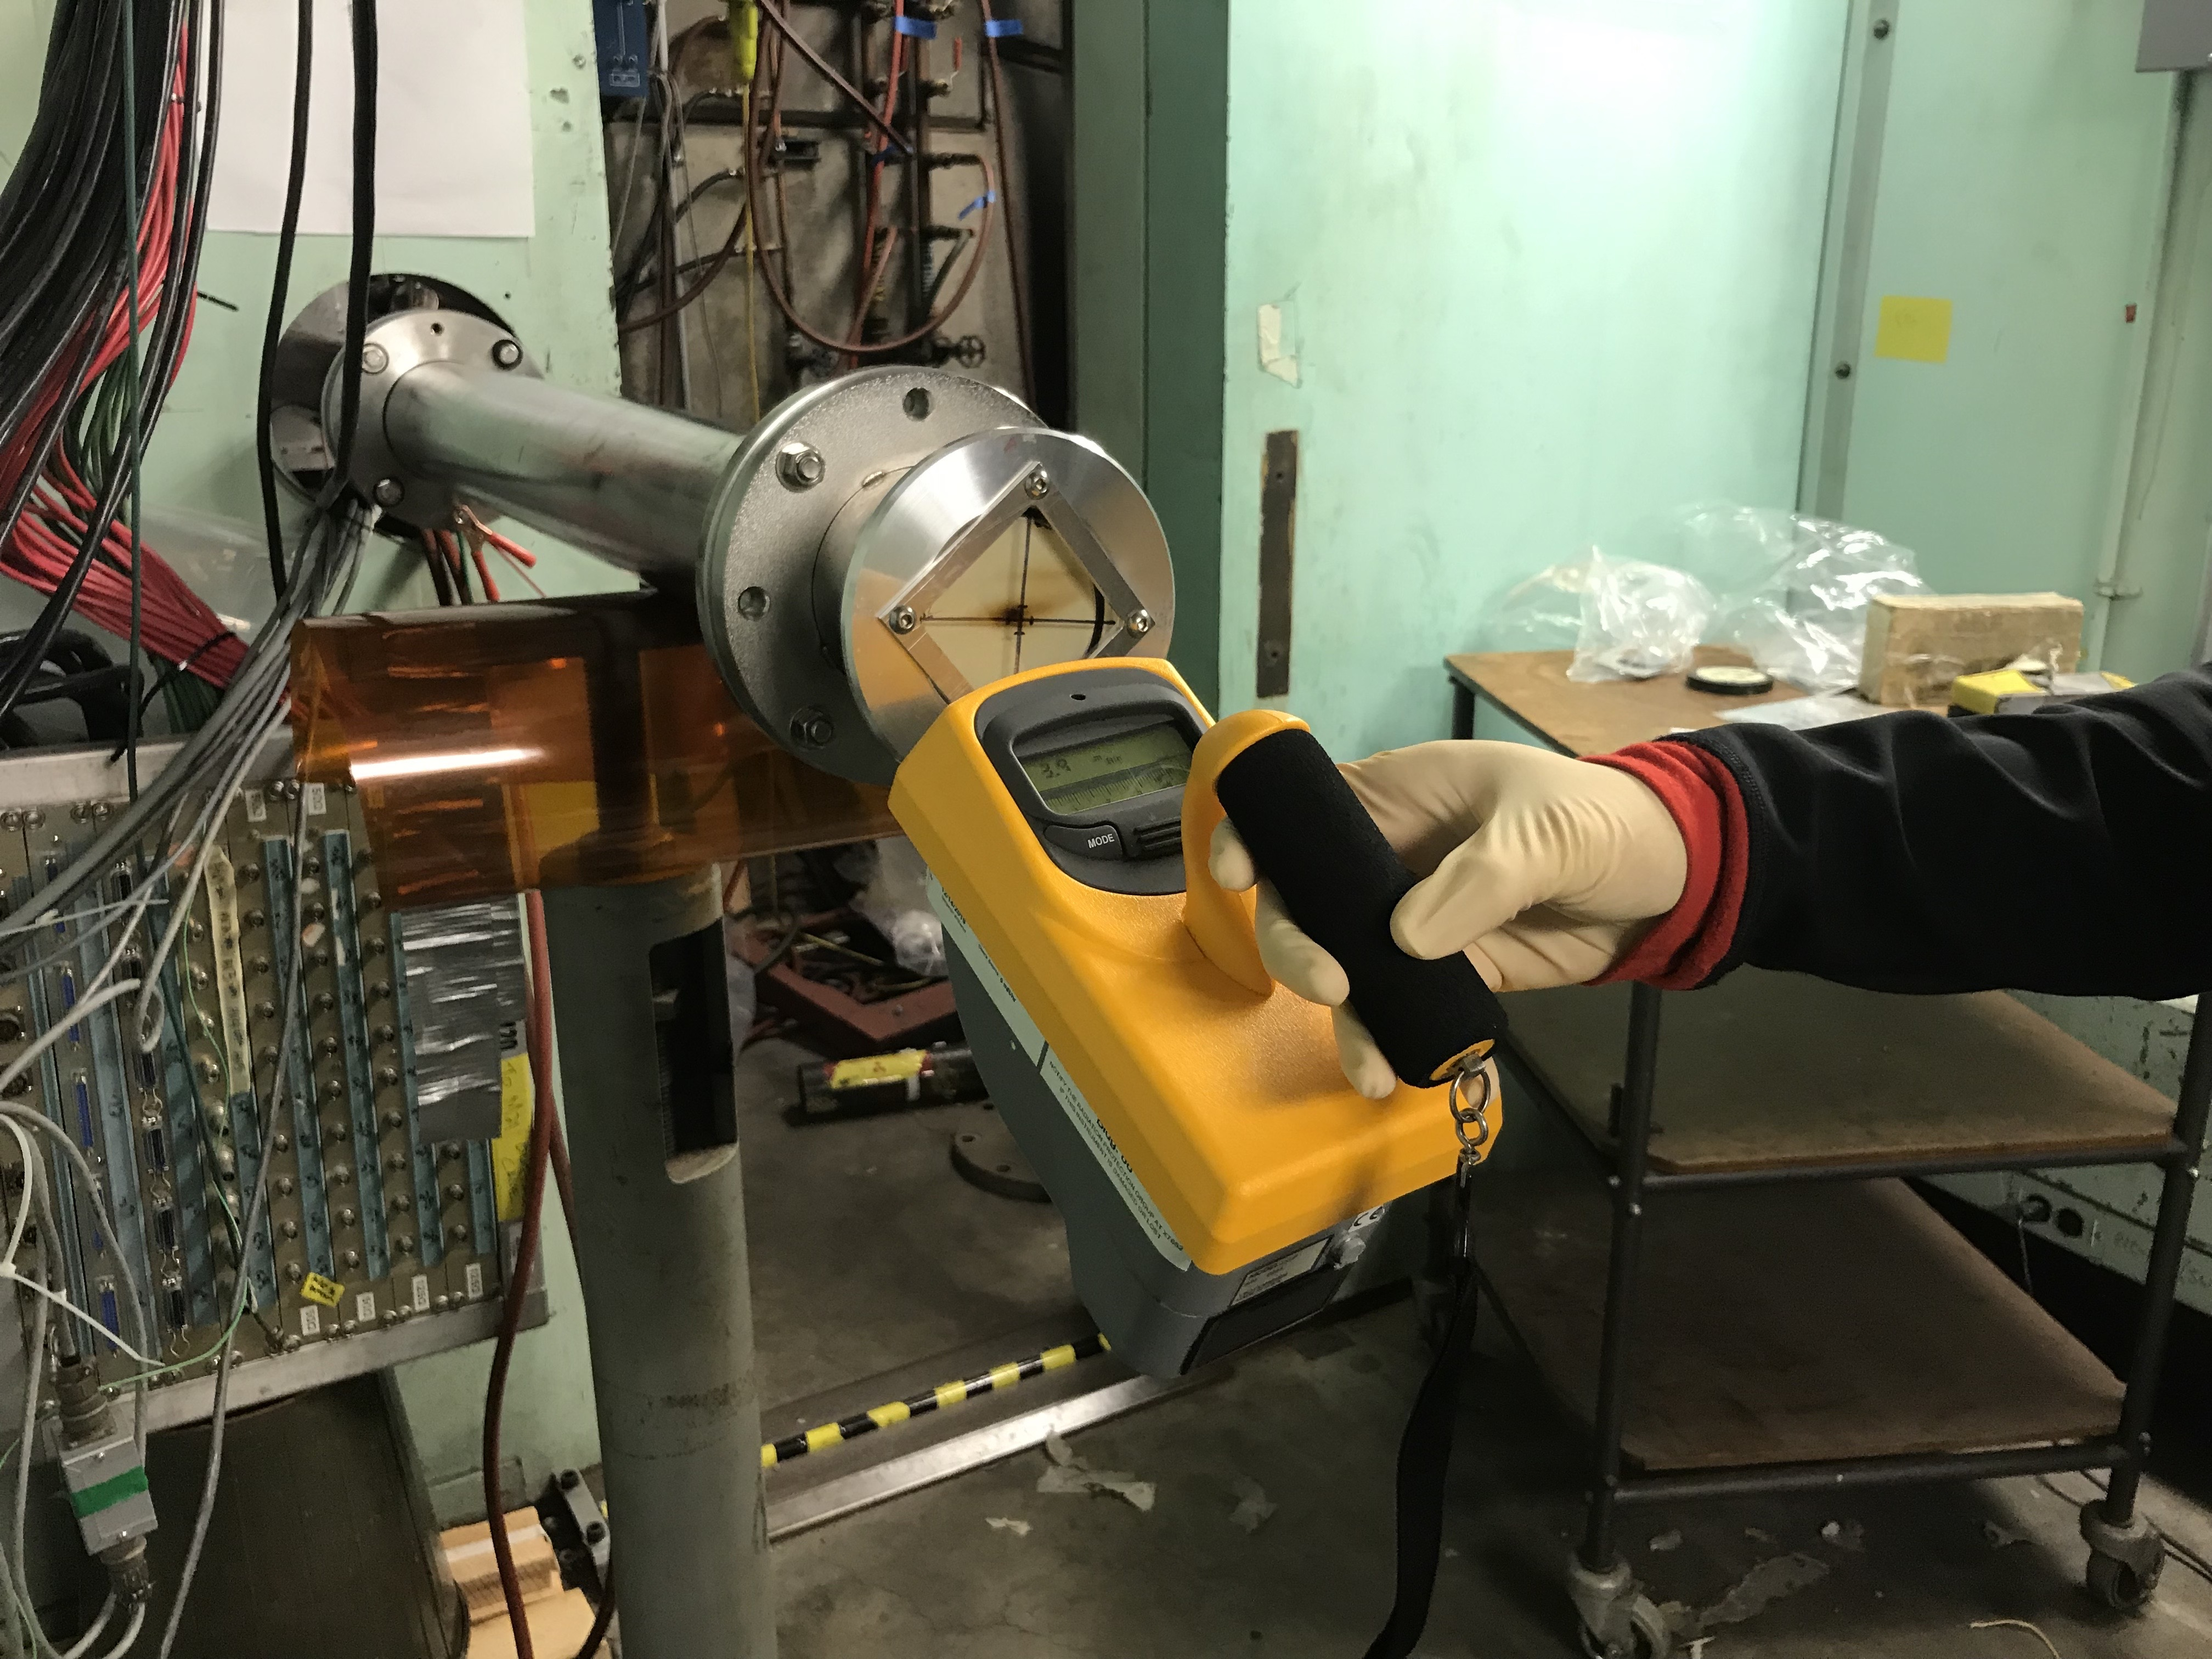
\includegraphics[width=6.6cm]{Experiment/phosphor_plate.JPG} }}%
    \caption{The figure shows the beamspot which could be visualized from the control room, and the borosilicate glass placed on the end of the beam tube. The dose present after the beam was on was always measured. }%
    \label{fig:tuning_phosphor+camera}%
\end{figure}

\begin{figure}
    \centering
    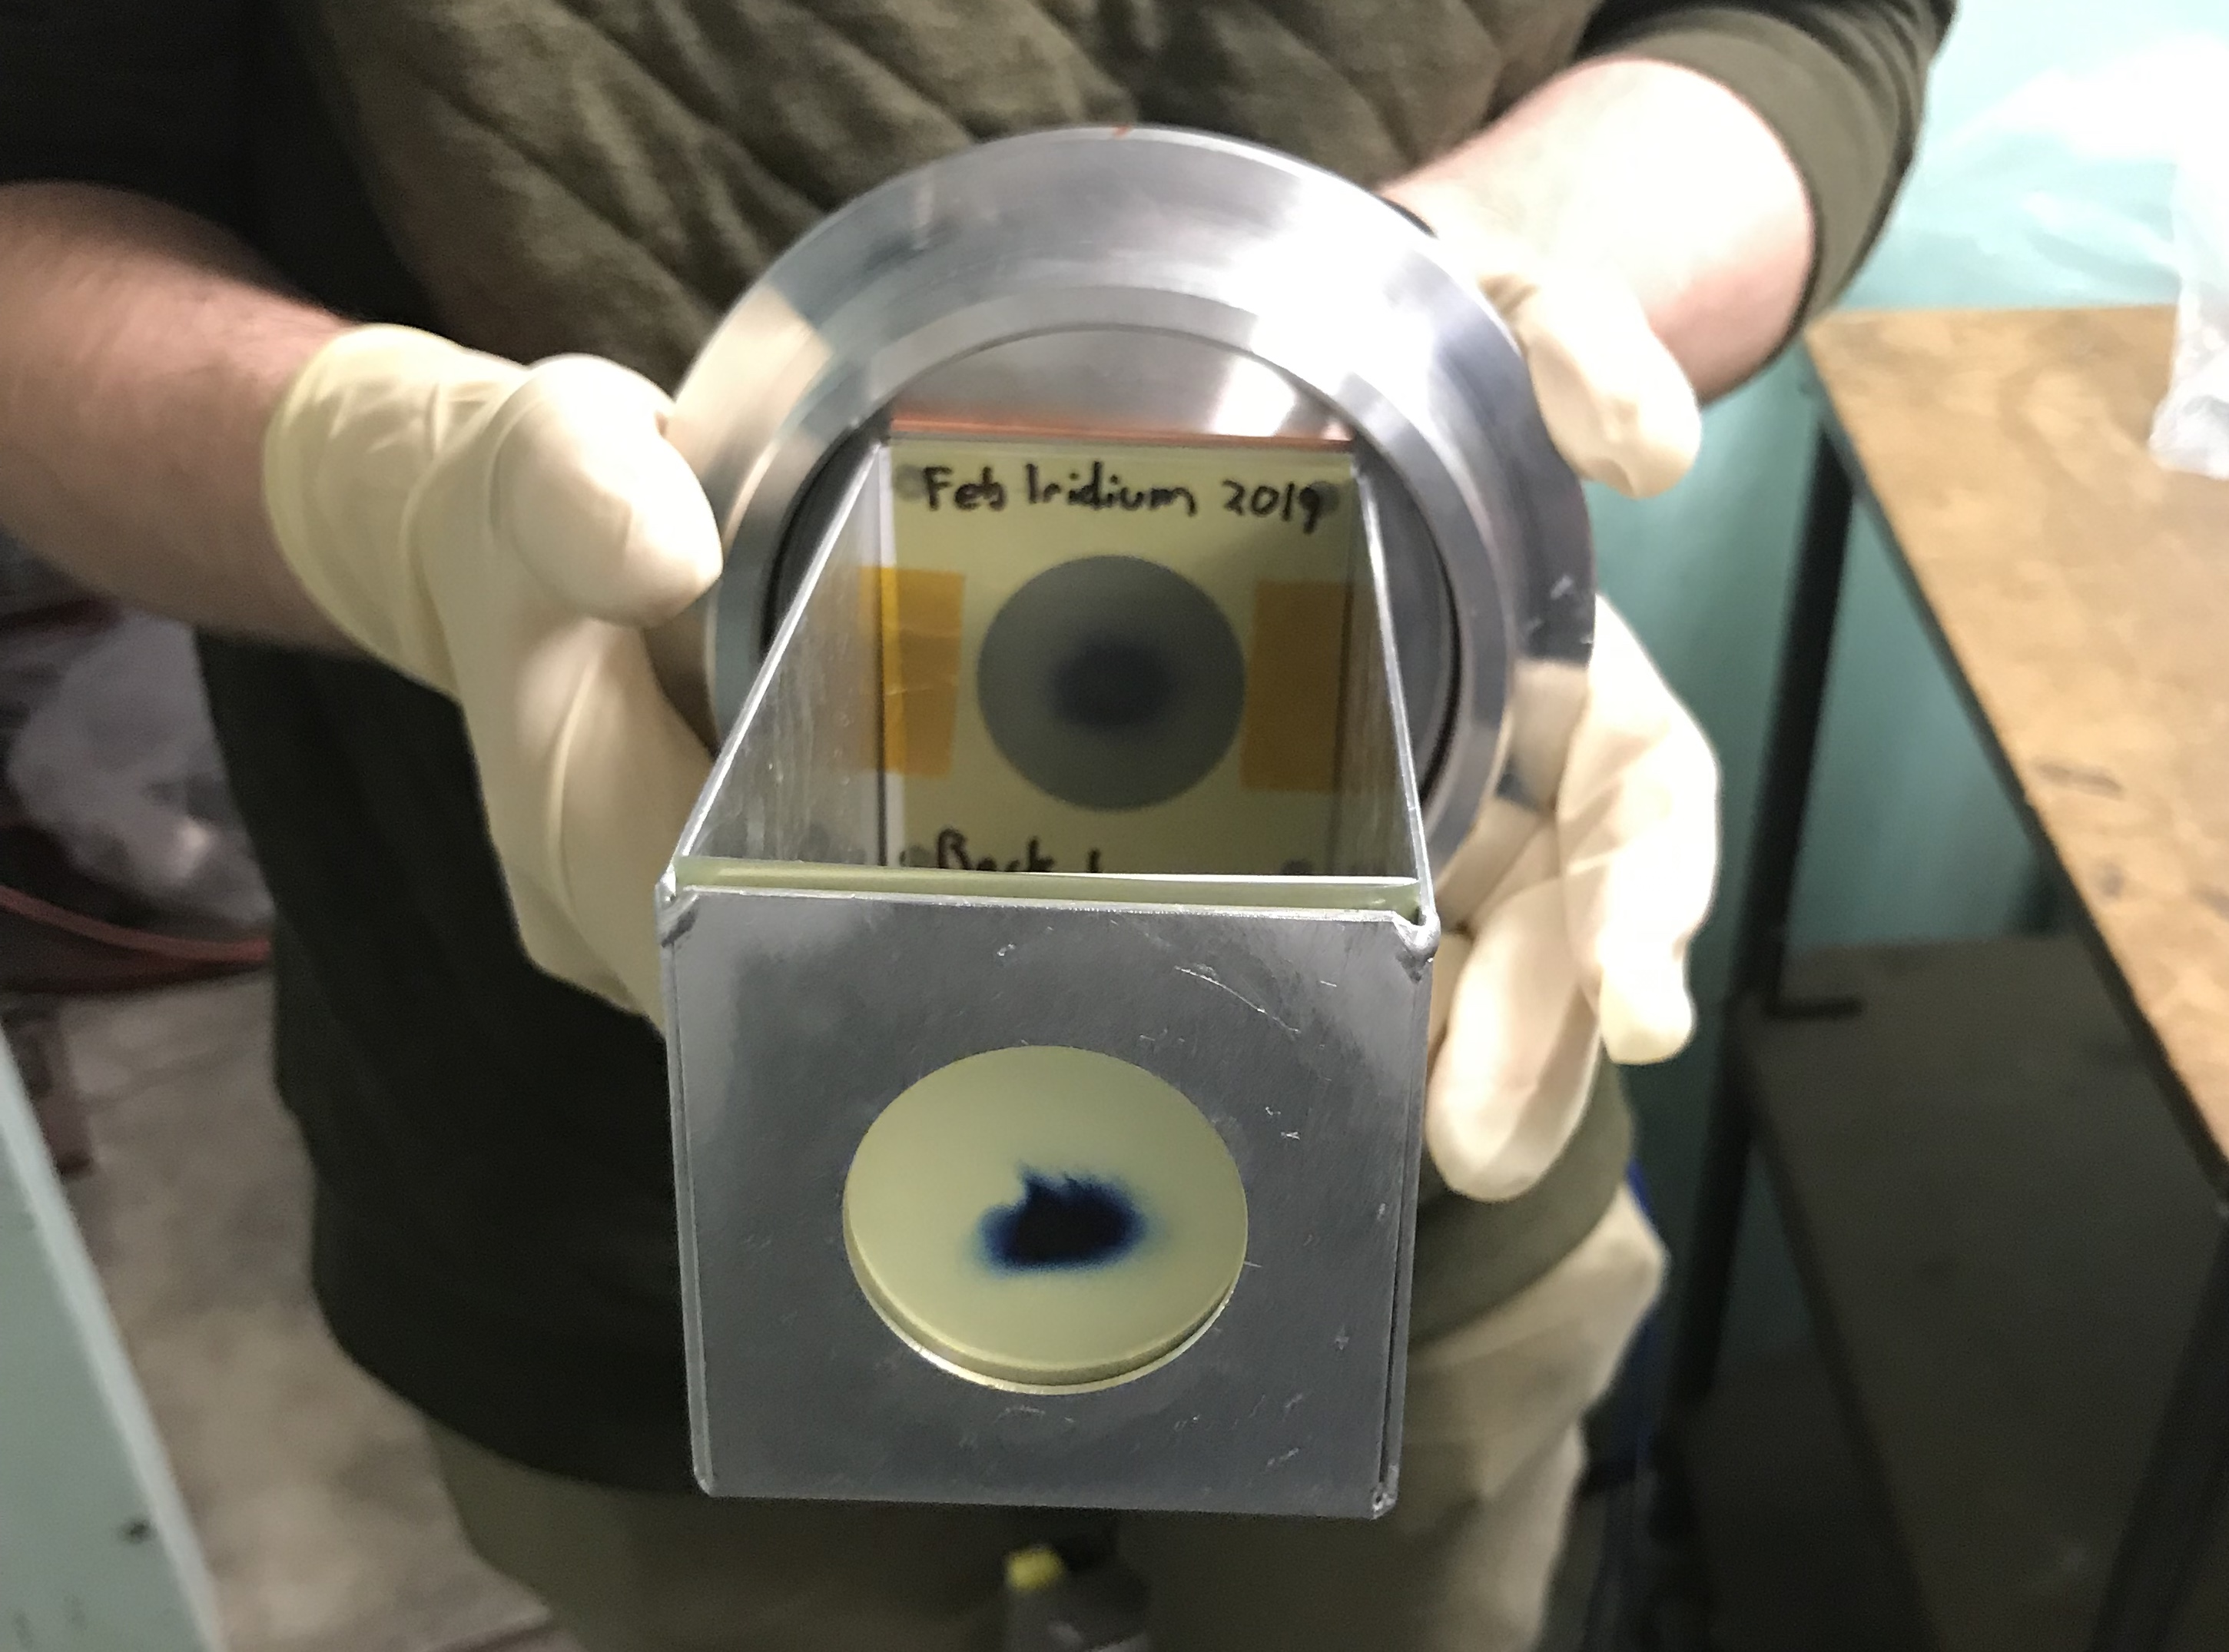
\includegraphics[width=0.7\textwidth]{Experiment/gafchromic_tune.jpg}
    \caption{Caption}
    \label{fig:tuning_gafchromic}
\end{figure}

\noindent
The beam efficiency transmission was calculated by measuring the the current at the Faraday cup right after the cyclotron vault (BS-02) and right before cave 0 (FC-01). BS-02 was measured to be 420 nA and FC-01 was measured to be 285 nA. This gave beam efficiency of transmission

$$\frac{FC-01}{BS-02}=67\% $$


\subsection{Irradiation of the target stack} \label{subsec:irradiation}
The irradiation lasted for one hour. The number of \textcolor{red}{charges collected??} was registered off the current integrator on the \textcolor{red}{electrically isolated beamline}, and registered evenly to ensure that the beamcurrent was more or less constant throughout the irradiation. After exactly one hour, the beam integrator read of $I\Delta t= 2314$ C, with full-scale amperes being $2\cdot10^{-7}$ A. The average beam current hitting the front of the stack was thus 

\begin{equation}
    \frac{2314\cdot 2\cdot10^{-7}}{3600 } = 128.5 \text{ nA}
\end{equation}

Before the beam was turned on, the beam tube had to be pumped down to a vacuum, to not attenuate the beam. The targetholder was placed in the end of the beam tube (\textcolor{red}{mounts of the end of an electrically-isolated beamline, (iron paper andrew)}). Figure \ref{fig:targetstack} shows how the targetholder was placed in the end of the beam tube. About ten minutes after end of beam, cave 0 was opened, and the targets were sealed in plastic bags to avoid contamination. The iridium foils counted from 15 minutes after end of beam on detector 7, and the other foils following up shortly after. All the foils were counted for ca. four weeks following end of beam on the various detectors, with short counts in the beginning to have good statistical data for the short-lived activities, and longer and longer counts as the shorter and medium-lived activities decayed out, to have good statistics (enough counts). The counts were done as jobscripts in the beginning, so that the same foil was measured multiple times.  Since the detectors were calibrated at various distances, the deadtime of the foils right after end of beam could be reduced, however, as high as  16-22\% deadtime was present, but reduced to less than 5\% within a cooling time of ca. 1 day after end of beam.
Due to the relatively long half-life of $^{193m}$Pt, and the weak gamma-ray, it was made sure that the single gamma-line was observed within a few days after end of beam, when the counts were longer. 

%The foils were counted at the seven different high purity germanium detectors for the following 4 weeks after end of beam, first short counts to get as many observations as possible of the short-lived activities and longer and longer counts as the times since end of beam passed, so that the counting statistics for the longer lived activities were good. 
\noindent 


\begin{figure}%
    \centering
    \subfloat[The target stack in target holder]{{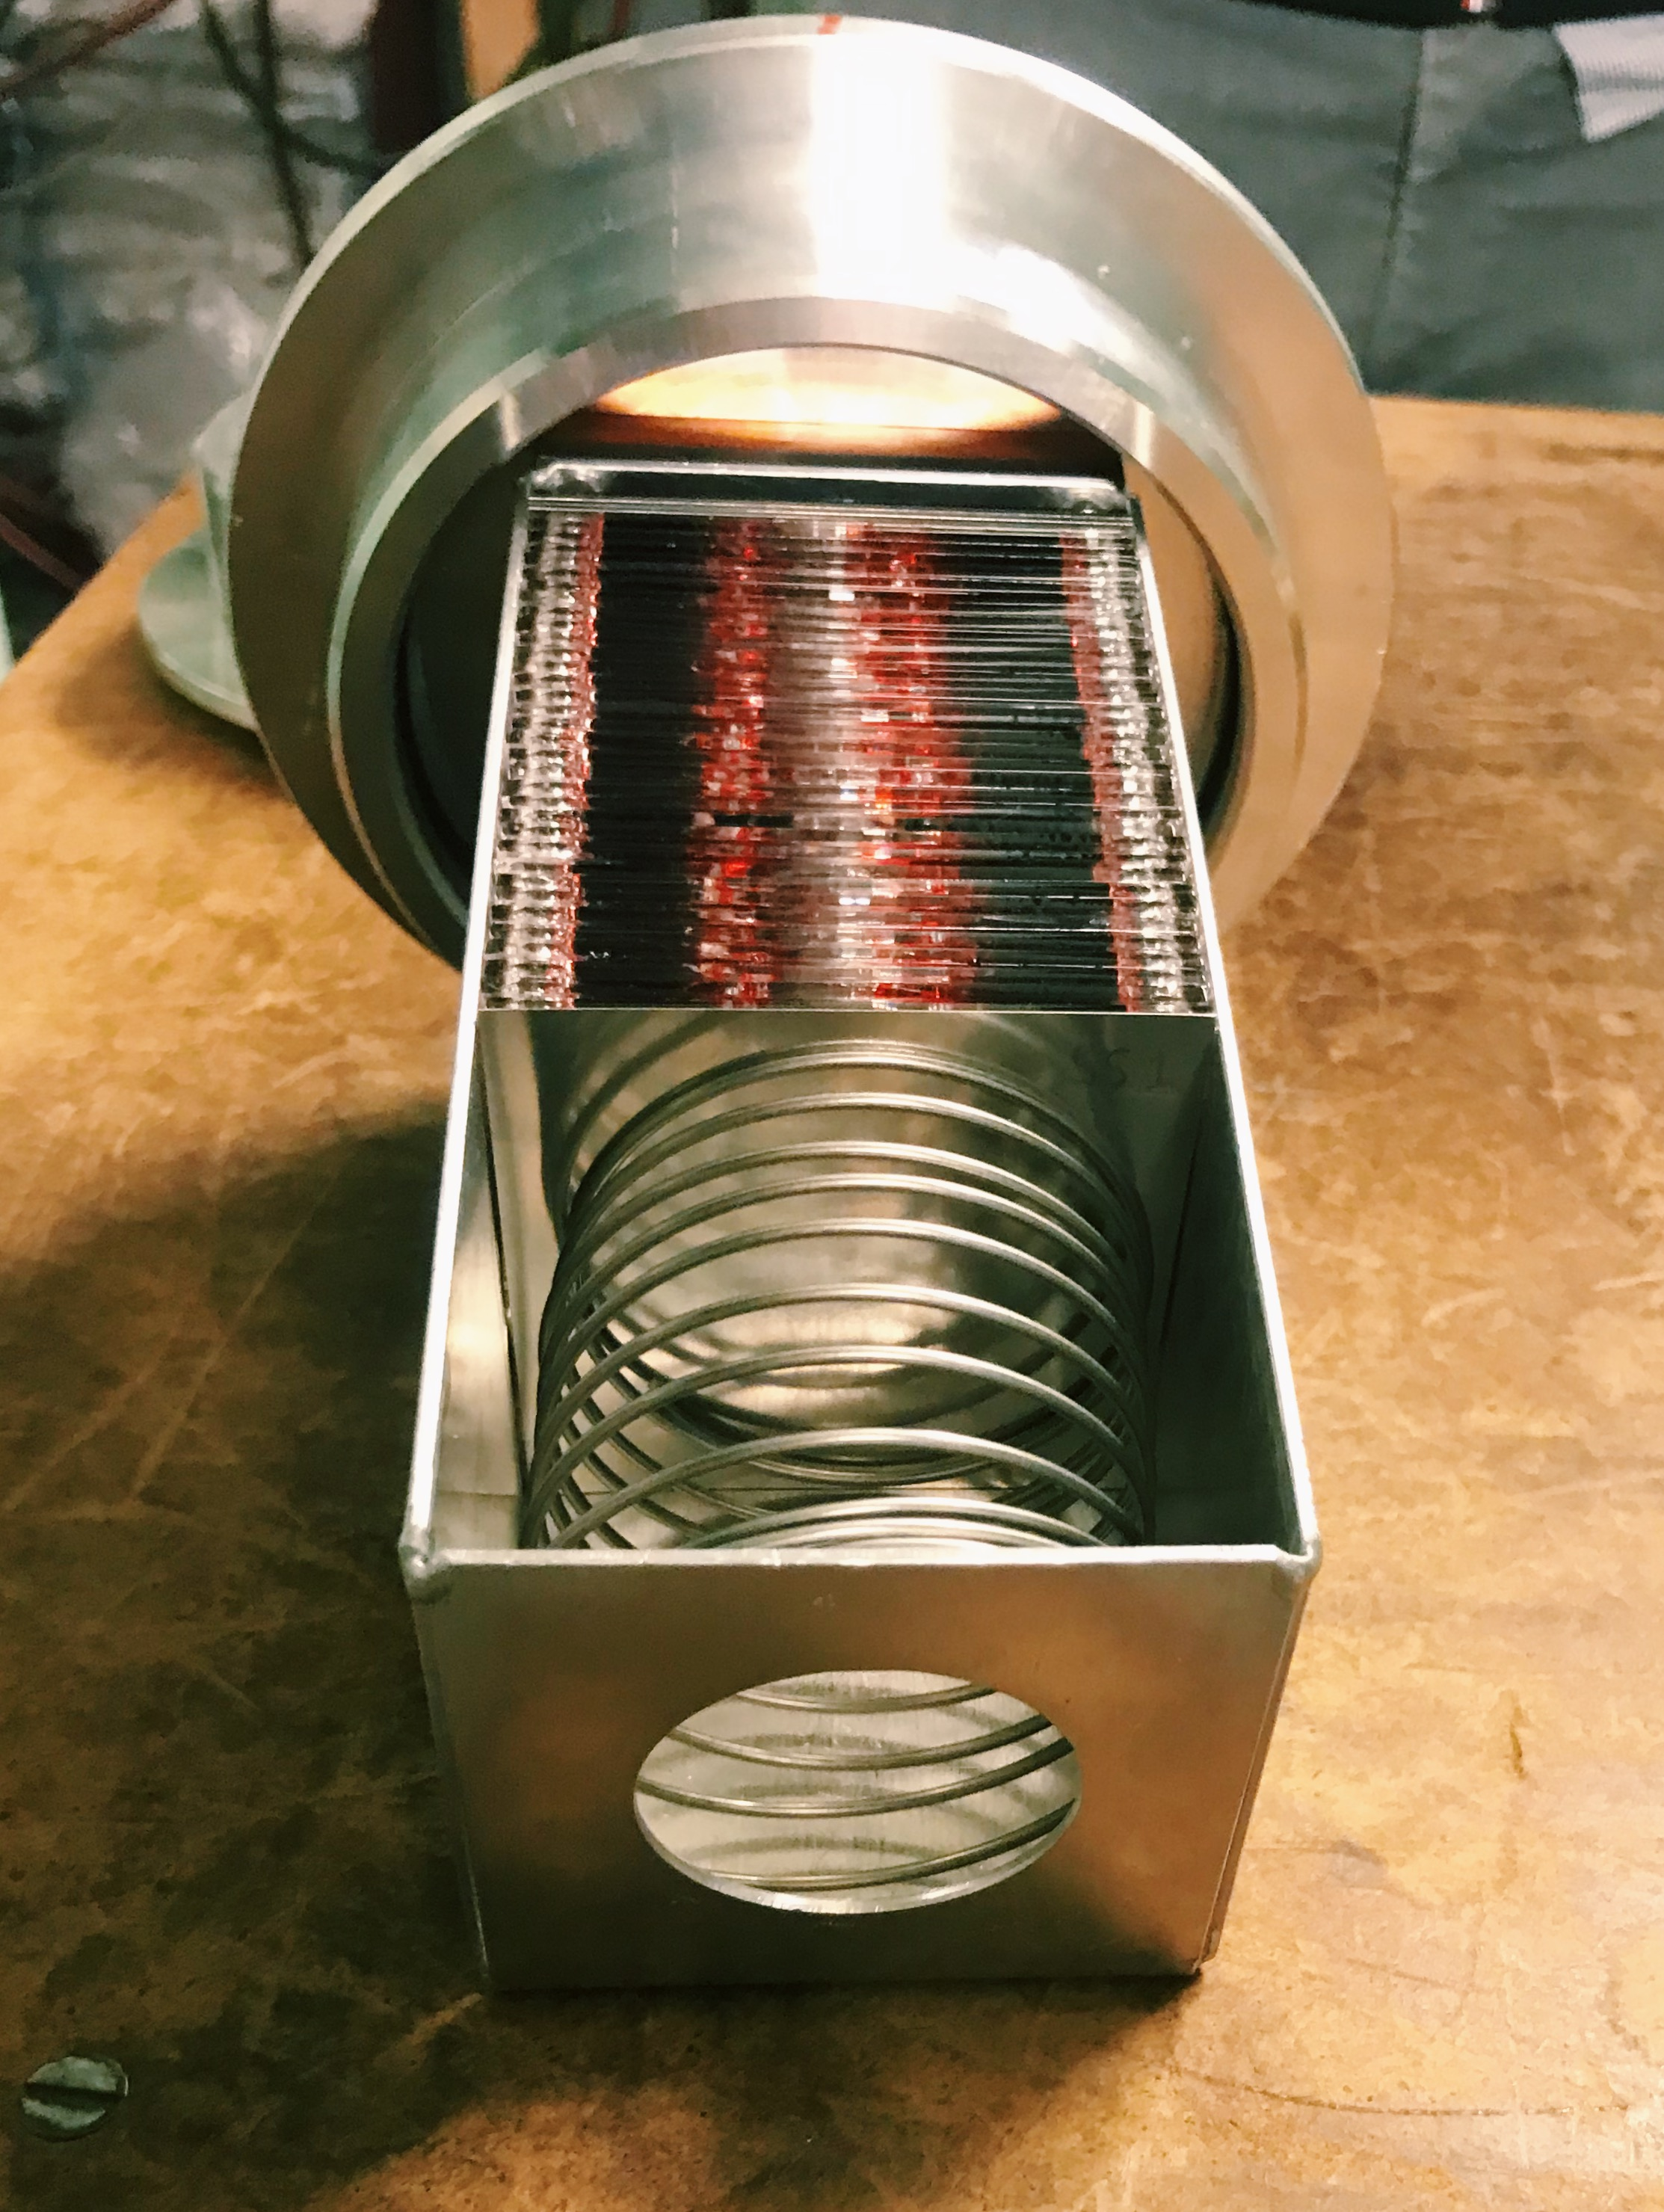
\includegraphics[width=6.6cm]{Experiment/stack.JPG} }}%
    \subfloat[Target holder placed in the end of beam tube]{{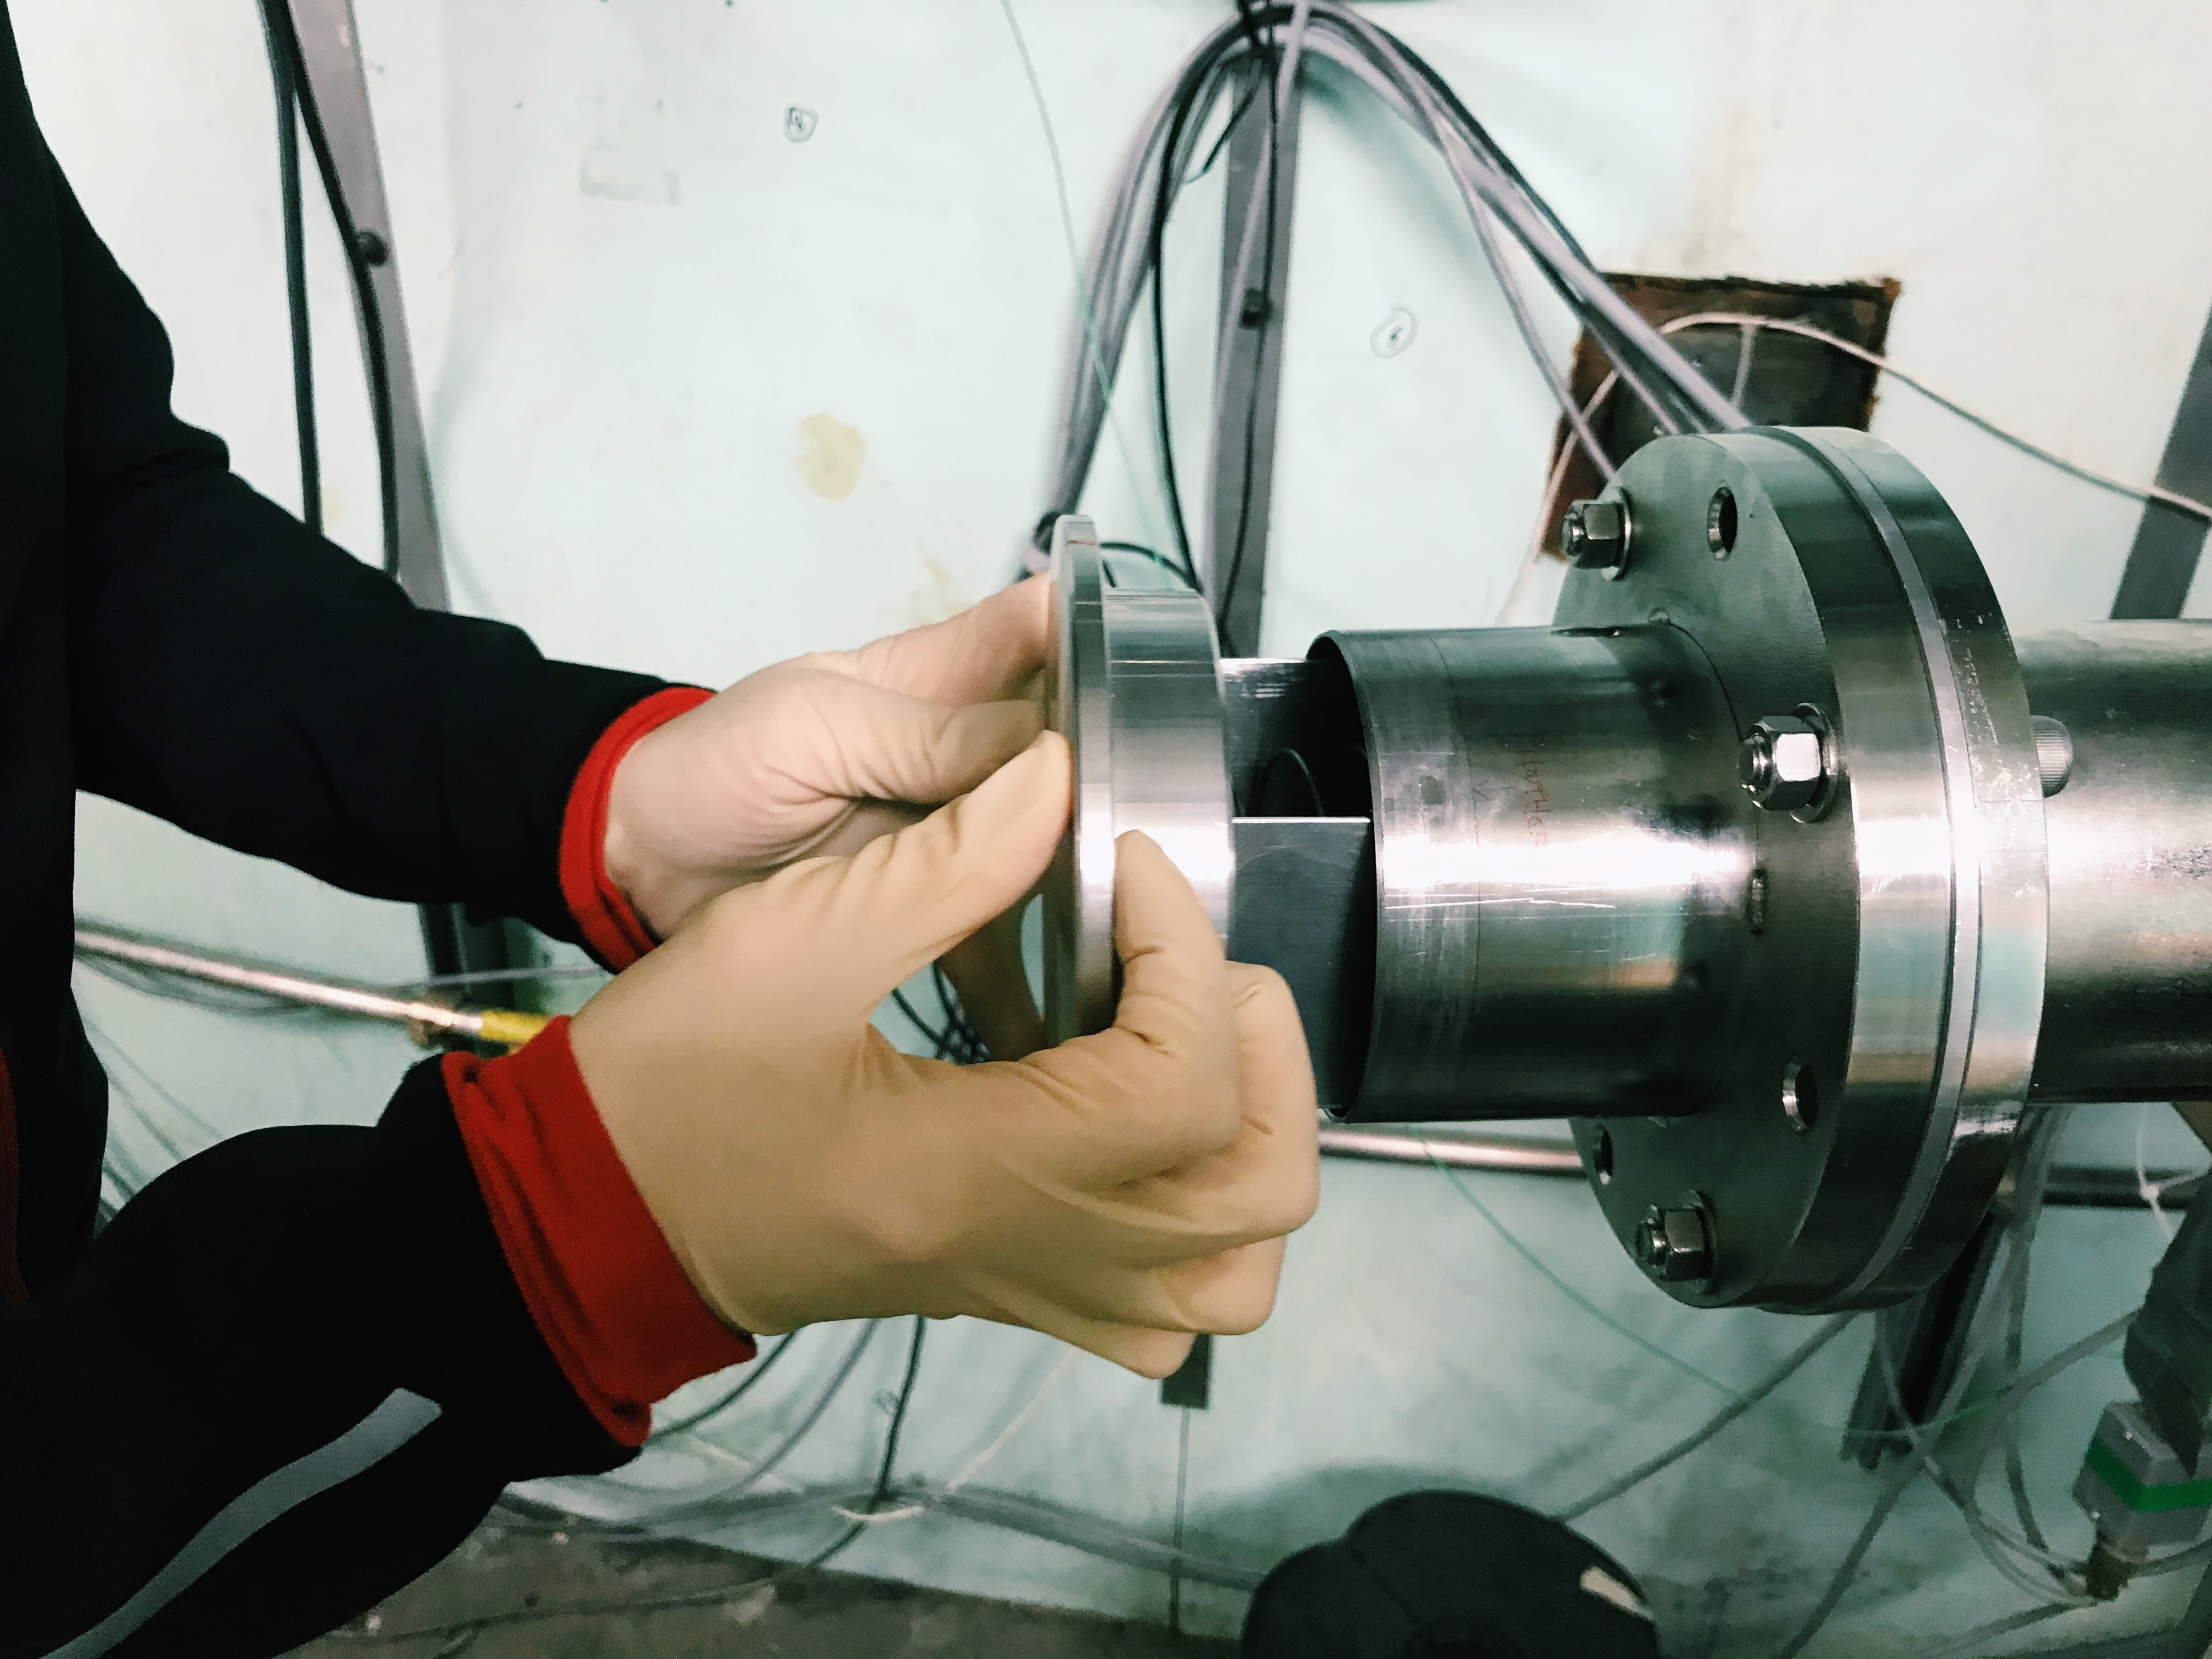
\includegraphics[width=6.6cm]{Experiment/tube.JPG} }}%
    \caption{Figure shows the target stack and how it was placed in the beam tube.}%
    \label{fig:targetstack}%
\end{figure}






\subsubsection{Intensity profile of the beam}

After irradiation, Gafchromic film were attached to the activated stainless steel in the front and the back of the stack, to obtain a spatial intensity profile of the beam. The activated film attached to the Gafhromic film can be seen in figure \ref{fig:SS1_gafchromic}. The radius of the activity from stainless on gafchromic film was used in the imaging process program ImageJ-1.52k, which is developed by the National Insititutes of Health and the Laboratory for Optical and Computational Instrumentation (wiki, imageJ). The gafchromic films were scanned alongside a ruler for scale comparison. Since the images are divided into pixels, a 3 \textcolor{red}{(why 3cm?)} cm linesegment was drawn alongside the ruler to set the scale to pixels/cm in the program. The intensity over the developed film was obtained by inverting the scanned image, and drawing a line segment along the beam spot that created a position dependent intensity array. The intensity profile can be fitted to a Gaussian, which is shown examplewise in figure \ref{fig:beamprofile}, which is the horizontal beam profile in the front and the back of the stack. In the assumption that the beam was underfilled, it was important to build confidence in that the beamspot was ca. 1 cm in diameter, which was done estimating the full width half maximum of the Gaussian profile. The FWHM over SS1 was 1.2017 cm horizontally ($\sigma^2=$0.2604 cm$^2$) and 1.1420 cm vertically ($\sigma^2=$0.2352 cm$^2$). The FWHM over SS2 was 0.6706 cm horizontally ($\sigma^2=$0.0811 cm$^2$) and 0.5783 cm vertically ($\sigma^2=$0.0603 cm$^2$). \\

\textcolor{red}{Normally the beam broadens throughout the stack due to scattering. As we can see, this not the case, since the beam is stopped in the targetstack, and therefor we do not know how much the beam truly scatters. This gives a higher uncertainty.  
The stainless steel (which consist of ..) has fast decay time. However since it emits beta-particles, the radius will slightly increase, and the true beam spot is slightly smaller. Thus the estimated FWHM values for SS1  seems to be within the criterion for underfilled targets. }



\begin{figure}
    \centering
    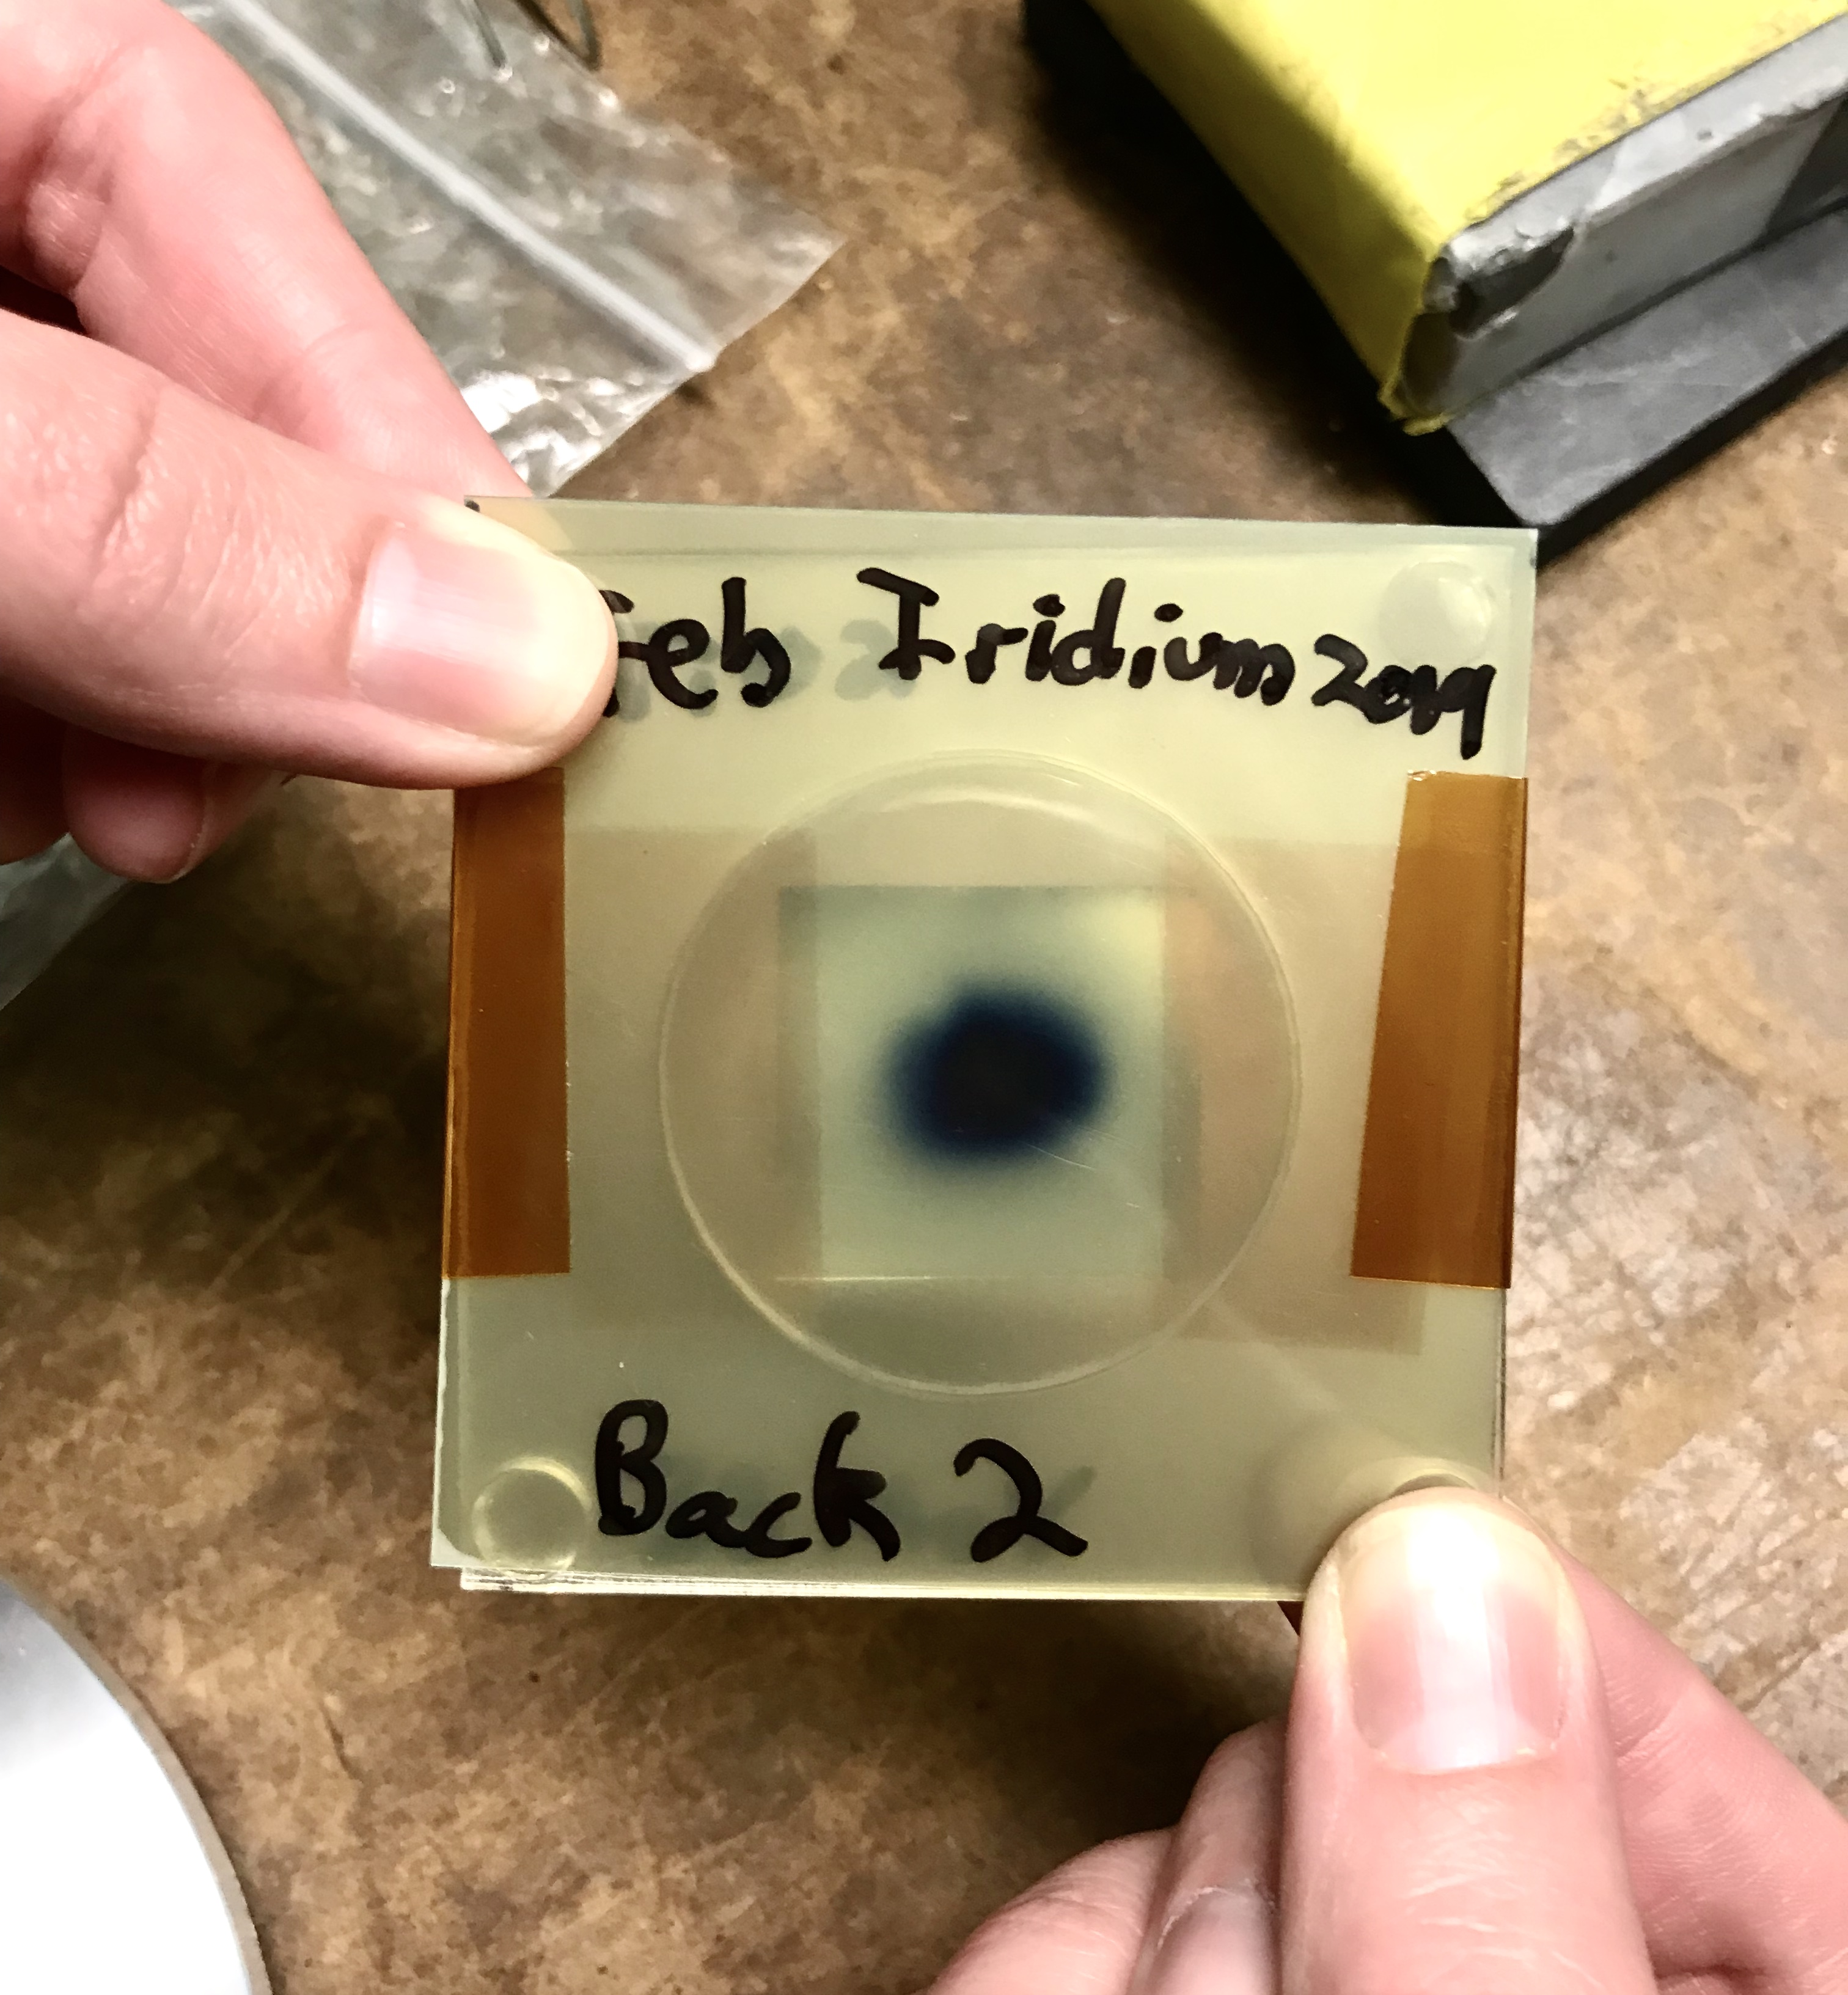
\includegraphics[width=0.3\textwidth]{Experiment/gafchromic_beamprofile.jpg}
    \caption{The gafcromic film on the activated SS1 foil. }
    \label{fig:SS1_gafchromic}
\end{figure}

\begin{figure}%
    \centering
    \subfloat[Horizontal intensity profile of SS1]{{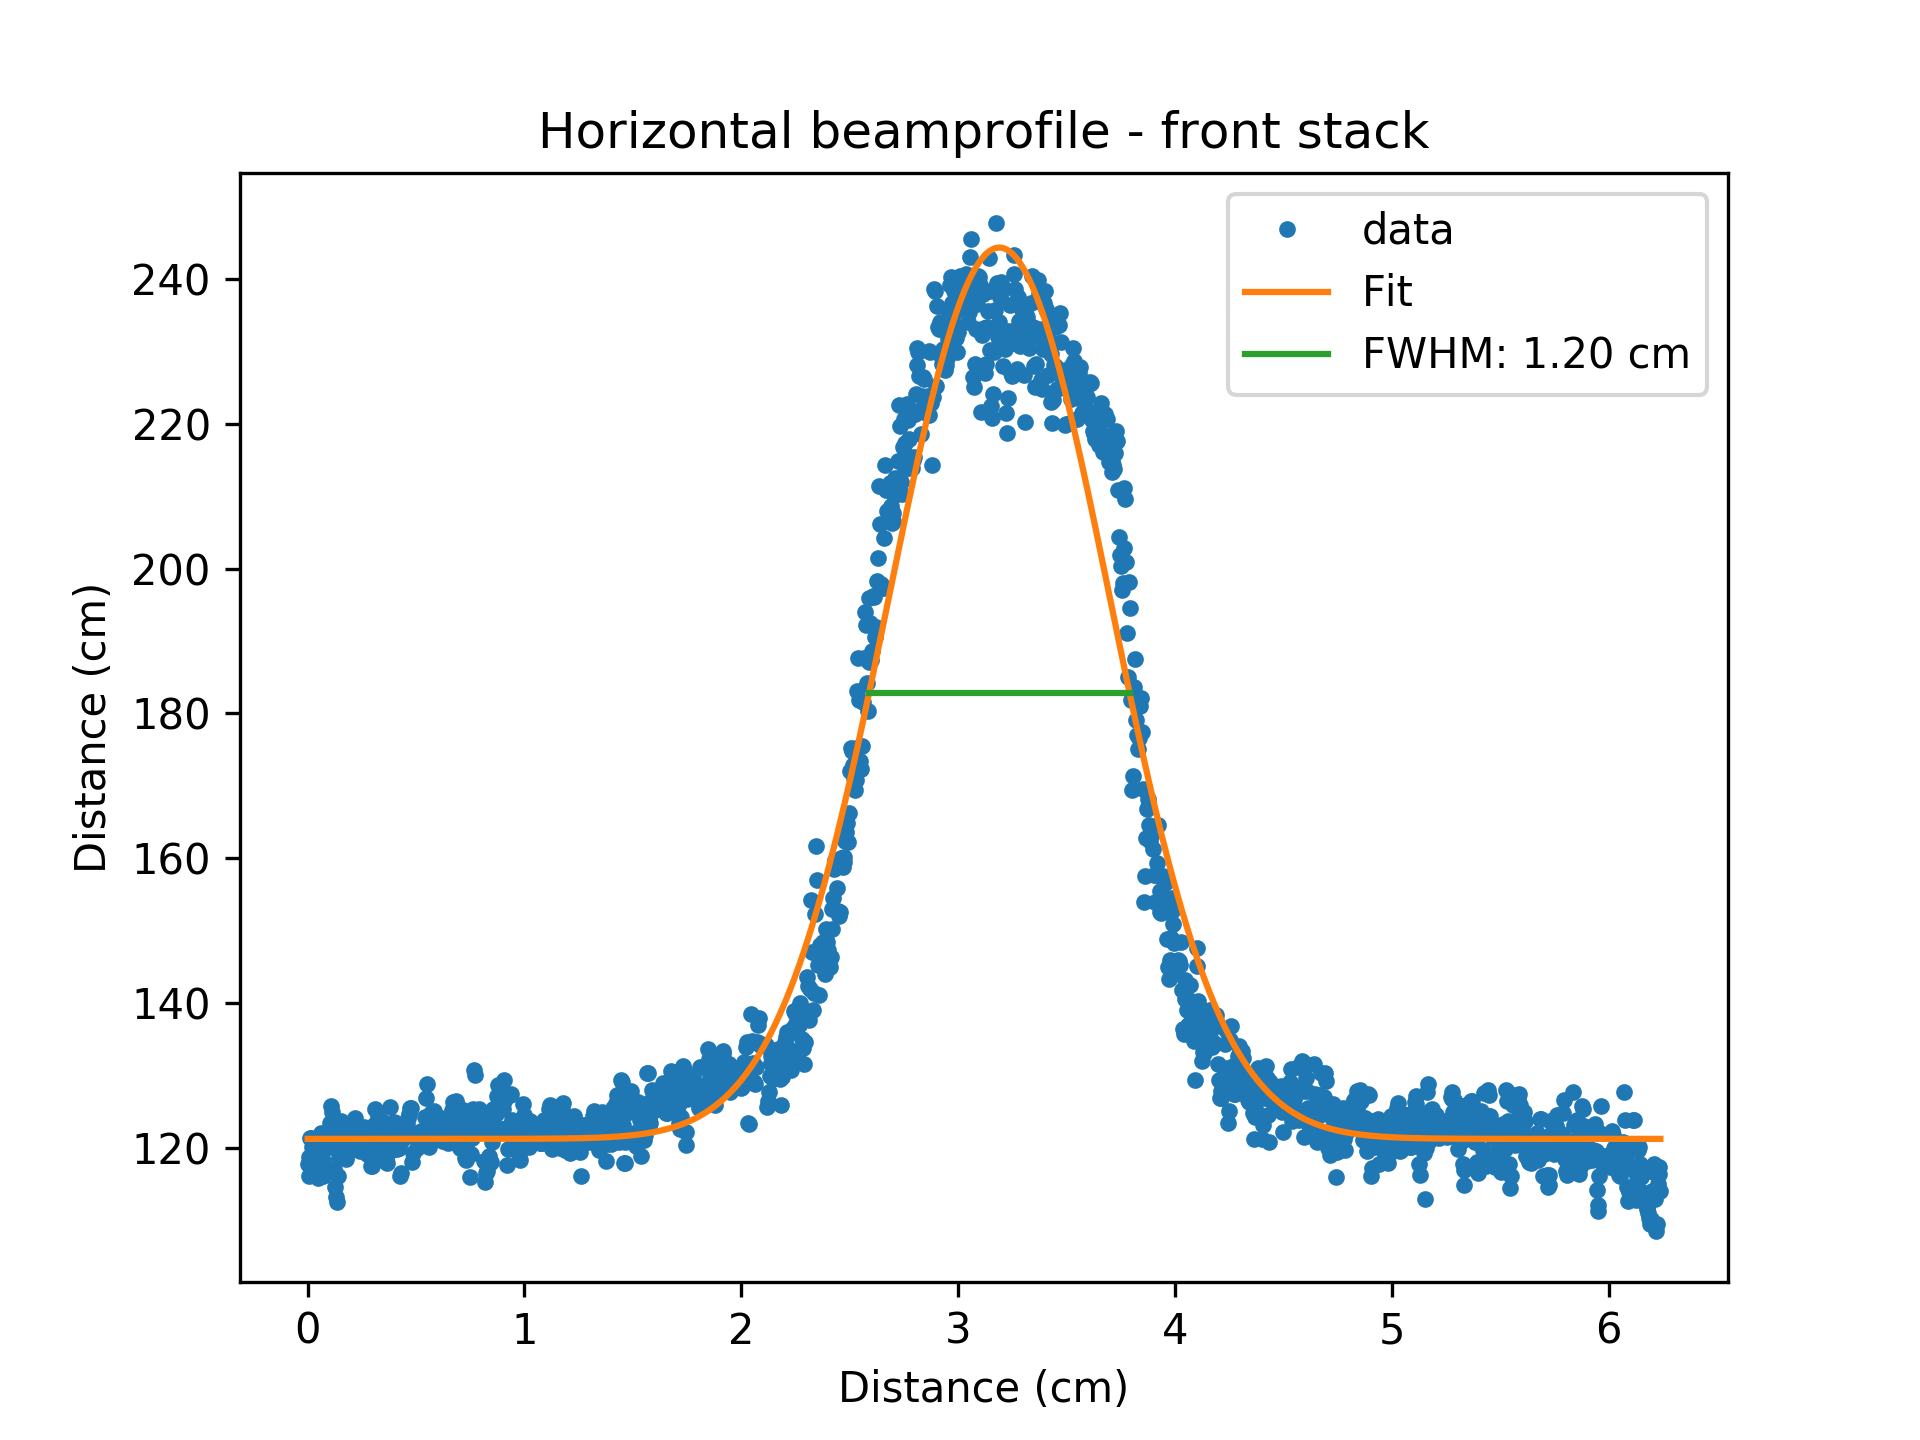
\includegraphics[width=6.6cm]{Experiment/ss_front_h.png} }}%
    
    \quad
    \subfloat[Horizontal intensity profile at SS2]{{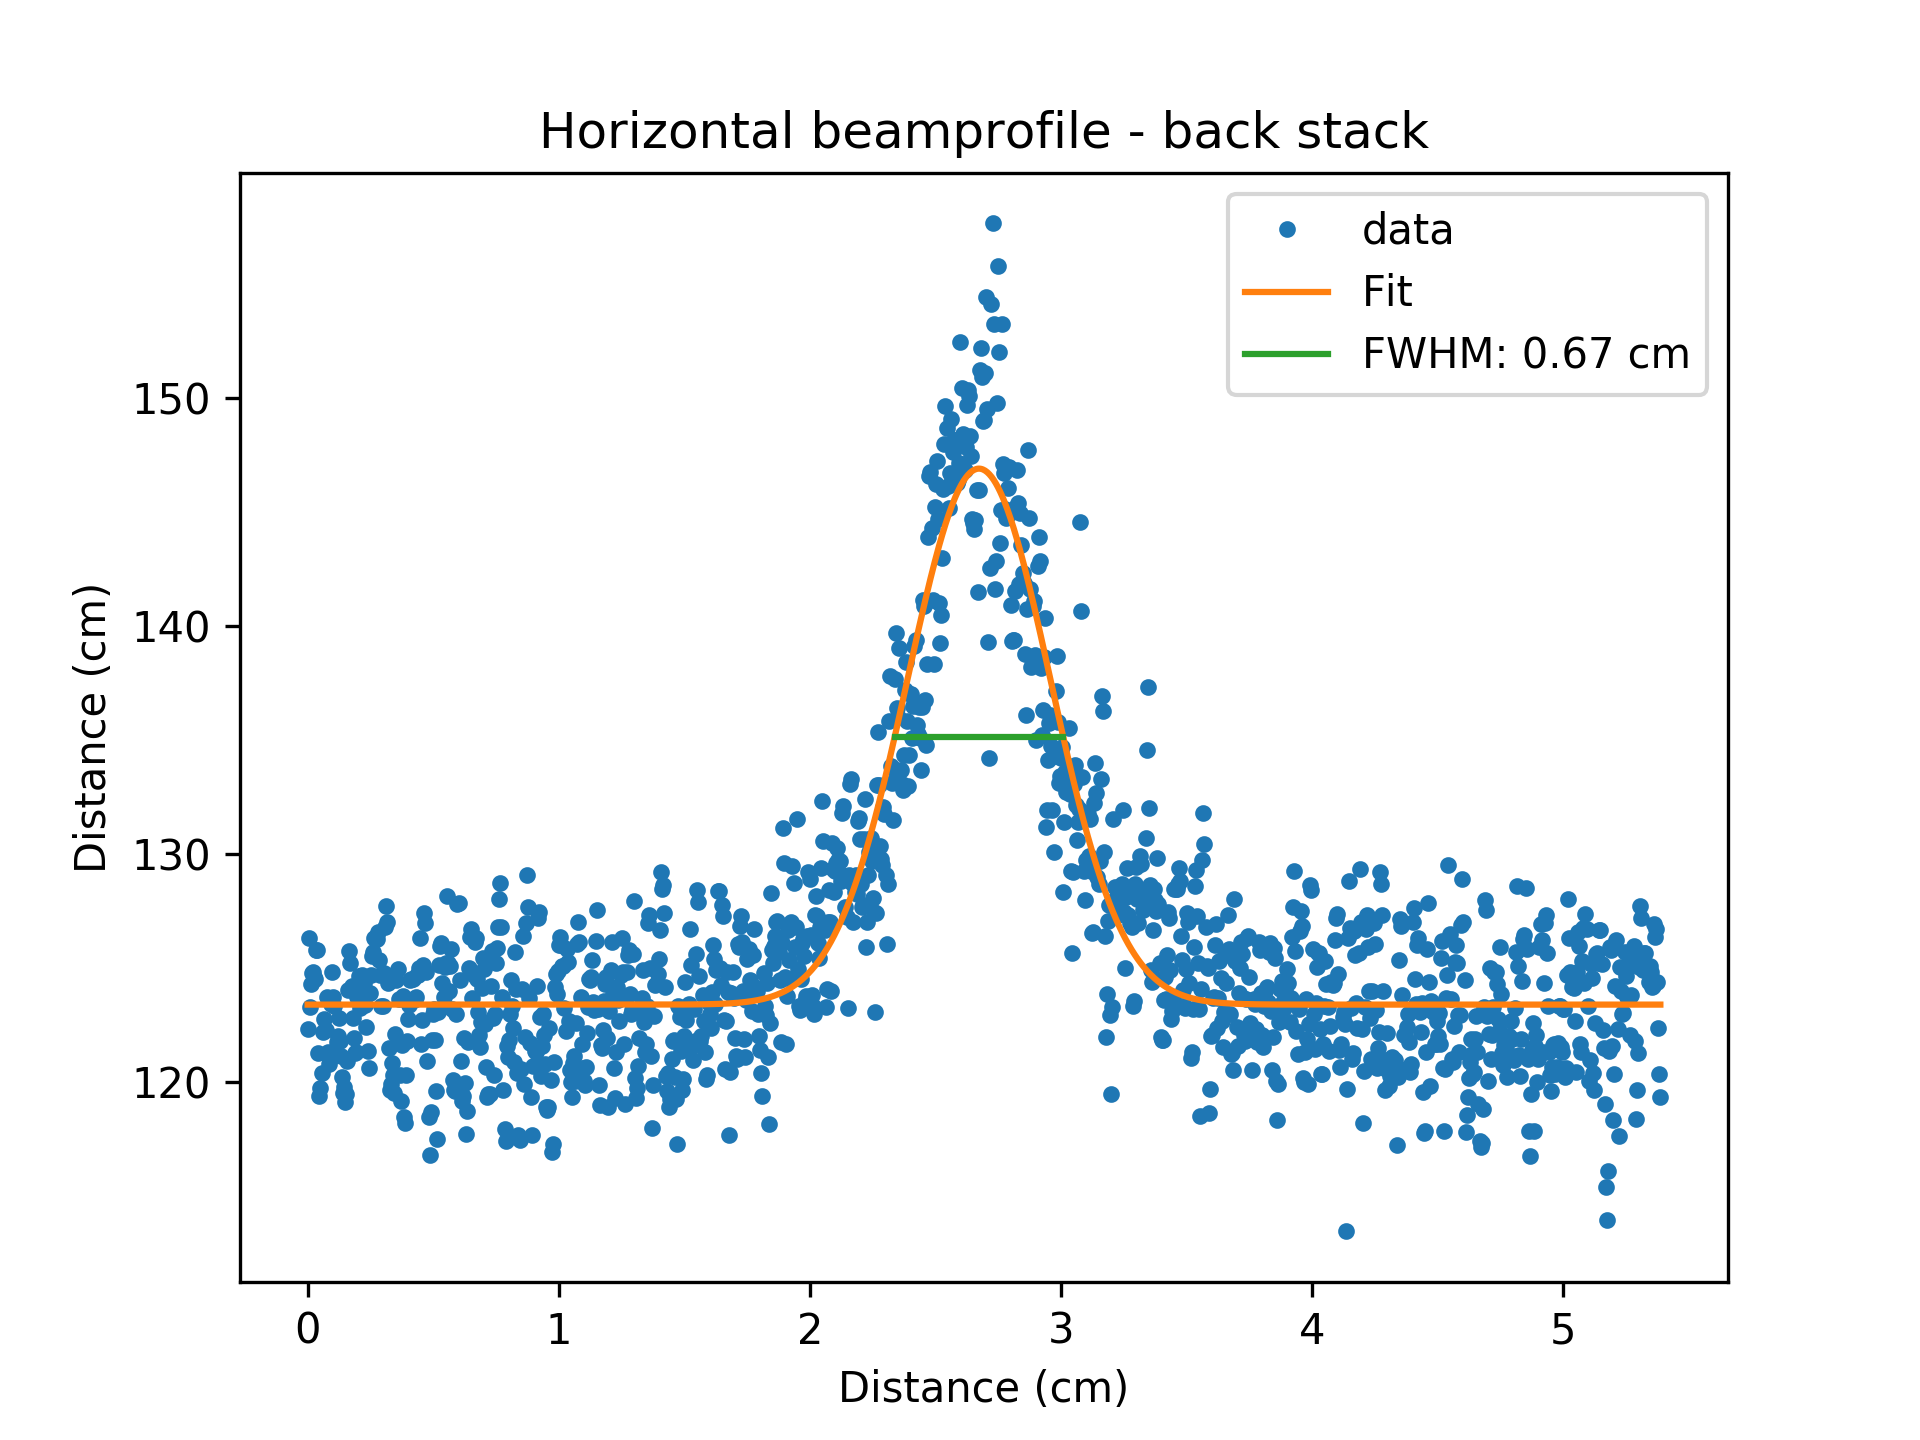
\includegraphics[width=6.6cm]{Experiment/ss_back_h.png} }}%
    \caption{Figure shows the intensity profile of the deuteron beam in the front and in the back of the stack horizontally.}%
    \label{fig:beamprofile}%
\end{figure}


\begin{figure}
    \centering
    \includegraphics[width=0.5\textwidth]{Experiment/cal_sources.png}
    \caption{The calibration point sources that were used in the efficiency calibration of the detector. ($^{22}$Na was excluded because it was difficult to work with. )}
    \label{fig:calsources}
\end{figure}

\begin{table}[]
    \centering
    \caption{The calibration point sources along with gamma lines used in the calibration of the detectors. * indicates that the value has been averaged over two peaks with similar energy, less than 1 keV. For the intensity its just added together. }
    \begin{tabular}{|cc|cc|cc|}
        \hline
        
         \multicolumn{2}{|c}{\makecell{^{137}Cs}} & \multicolumn{2}{c}{\makecell{^{133}Ba}} & \multicolumn{2}{c|}{\makecell{^{152}Eu}}\\
         %\hline 
         \Xhline{2\arrayrulewidth}
         \makecell{E_\gamma}& \makecell{I_\gamma}&\makecell{E_\gamma}& \makecell{I_\gamma}& \makecell{E_\gamma}& \makecell{I_\gamma}\\
         \hline
         \makecell{32.005^*} & \makecell{5.63^*} & \makecell{53.1622} & \makecell{2.14} & \makecell{121.7817} & \makecell{28.53}\\
         
         \makecell{36.3405^*} & \makecell{1.02^*} & \makecell{80.9979} & \makecell{32.9} & \makecell{244.6979} & \makecell{7.55}\\
         
         \makecell{661.657} & \makecell{85.10} & \makecell{160.6120} & \makecell{0.638} & \makecell{295.9387} & \makecell{0.440}\\
         
          &  & \makecell{223.2368} & \makecell{0.453} & \makecell{344.2785} & \makecell{26.5}\\
         
          &  & \makecell{276.3989} & \makecell{7.16} & \makecell{367.7891} & \makecell{0.859}\\
         
          &  & \makecell{302.8508} & \makecell{18.34} & \makecell{411.1165} & \makecell{2.237}\\
          
          
          &  & \makecell{356.0129} & \makecell{62.05} & \makecell{244.4853^*} & \makecell{3.125^*}\\
          
           &  & \makecell{383.8485} & \makecell{8.94} & \makecell{503.467} & \makecell{0.1524}\\
           
           &  & \makecell{} & \makecell{} & \makecell{586.2648} & \makecell{0.455}\\
           
           &  & \makecell{} & \makecell{} & \makecell{678.623} & \makecell{0.473}\\
           &  & \makecell{} & \makecell{} & \makecell{688.670} & \makecell{0.856}\\
           
           &  & \makecell{} & \makecell{} & \makecell{719.353^*} & \makecell{0.345^*}\\
           &  & \makecell{} & \makecell{} & \makecell{778.9045} & \makecell{12.93}\\
           &  & \makecell{} & \makecell{} & \makecell{810.451} & \makecell{0.317}\\
           &  & \makecell{} & \makecell{} & \makecell{867.380} & \makecell{4.23}\\
           &  & \makecell{} & \makecell{} & \makecell{963.712^*} & \makecell{14.65^*}\\
           &  & \makecell{} & \makecell{} & \makecell{1112.076} & \makecell{13.67}\\
           &  & \makecell{} & \makecell{} & \makecell{1212.948} & \makecell{1.415}\\
           &  & \makecell{} & \makecell{} & \makecell{1299.142} & \makecell{1.633}\\
           &  & \makecell{} & \makecell{} & \makecell{1408.013} & \makecell{20.87}\\
        %\makecell{^{137}Cs} & \makecell{^{133}Ba} & \makecell{^{152}Eu} \\
        \hline 
   
        \hline
    \end{tabular}
    \label{table:calibration_gammas}
\end{table}


\begin{comment}
\begin{table}[]
    \centering
    \caption{Table shows the geometry of the different detectors. }
    \begin{tabular}{|c|c|c|}
        \hline\textbf{}
        Detector & Geometry & Dimension \\
        \hline 
        \makecell{Detector 1} & \makecell{..} & \makecell{..} \\
        \makecell{Detector 1} & \makecell{..} & \makecell{..} \\      
        \makecell{Detector 3} & \makecell{..} & \makecell{..} \\     
        \makecell{Detector 4} & \makecell{..} & \makecell{..} \\  
        \makecell{Detector 5} & \makecell{..} & \makecell{..} \\    
        \makecell{Detector 6} & \makecell{..} & \makecell{..} \\      
        \makecell{Detector 7} & \makecell{..} & \makecell{..} \\     
        \hline
    \end{tabular}
    \label{tab:detector_characteristics}
\end{table}
\end{comment}

\



\begin{comment}
\begin{figure}%
    \centering
    \subfloat[]{{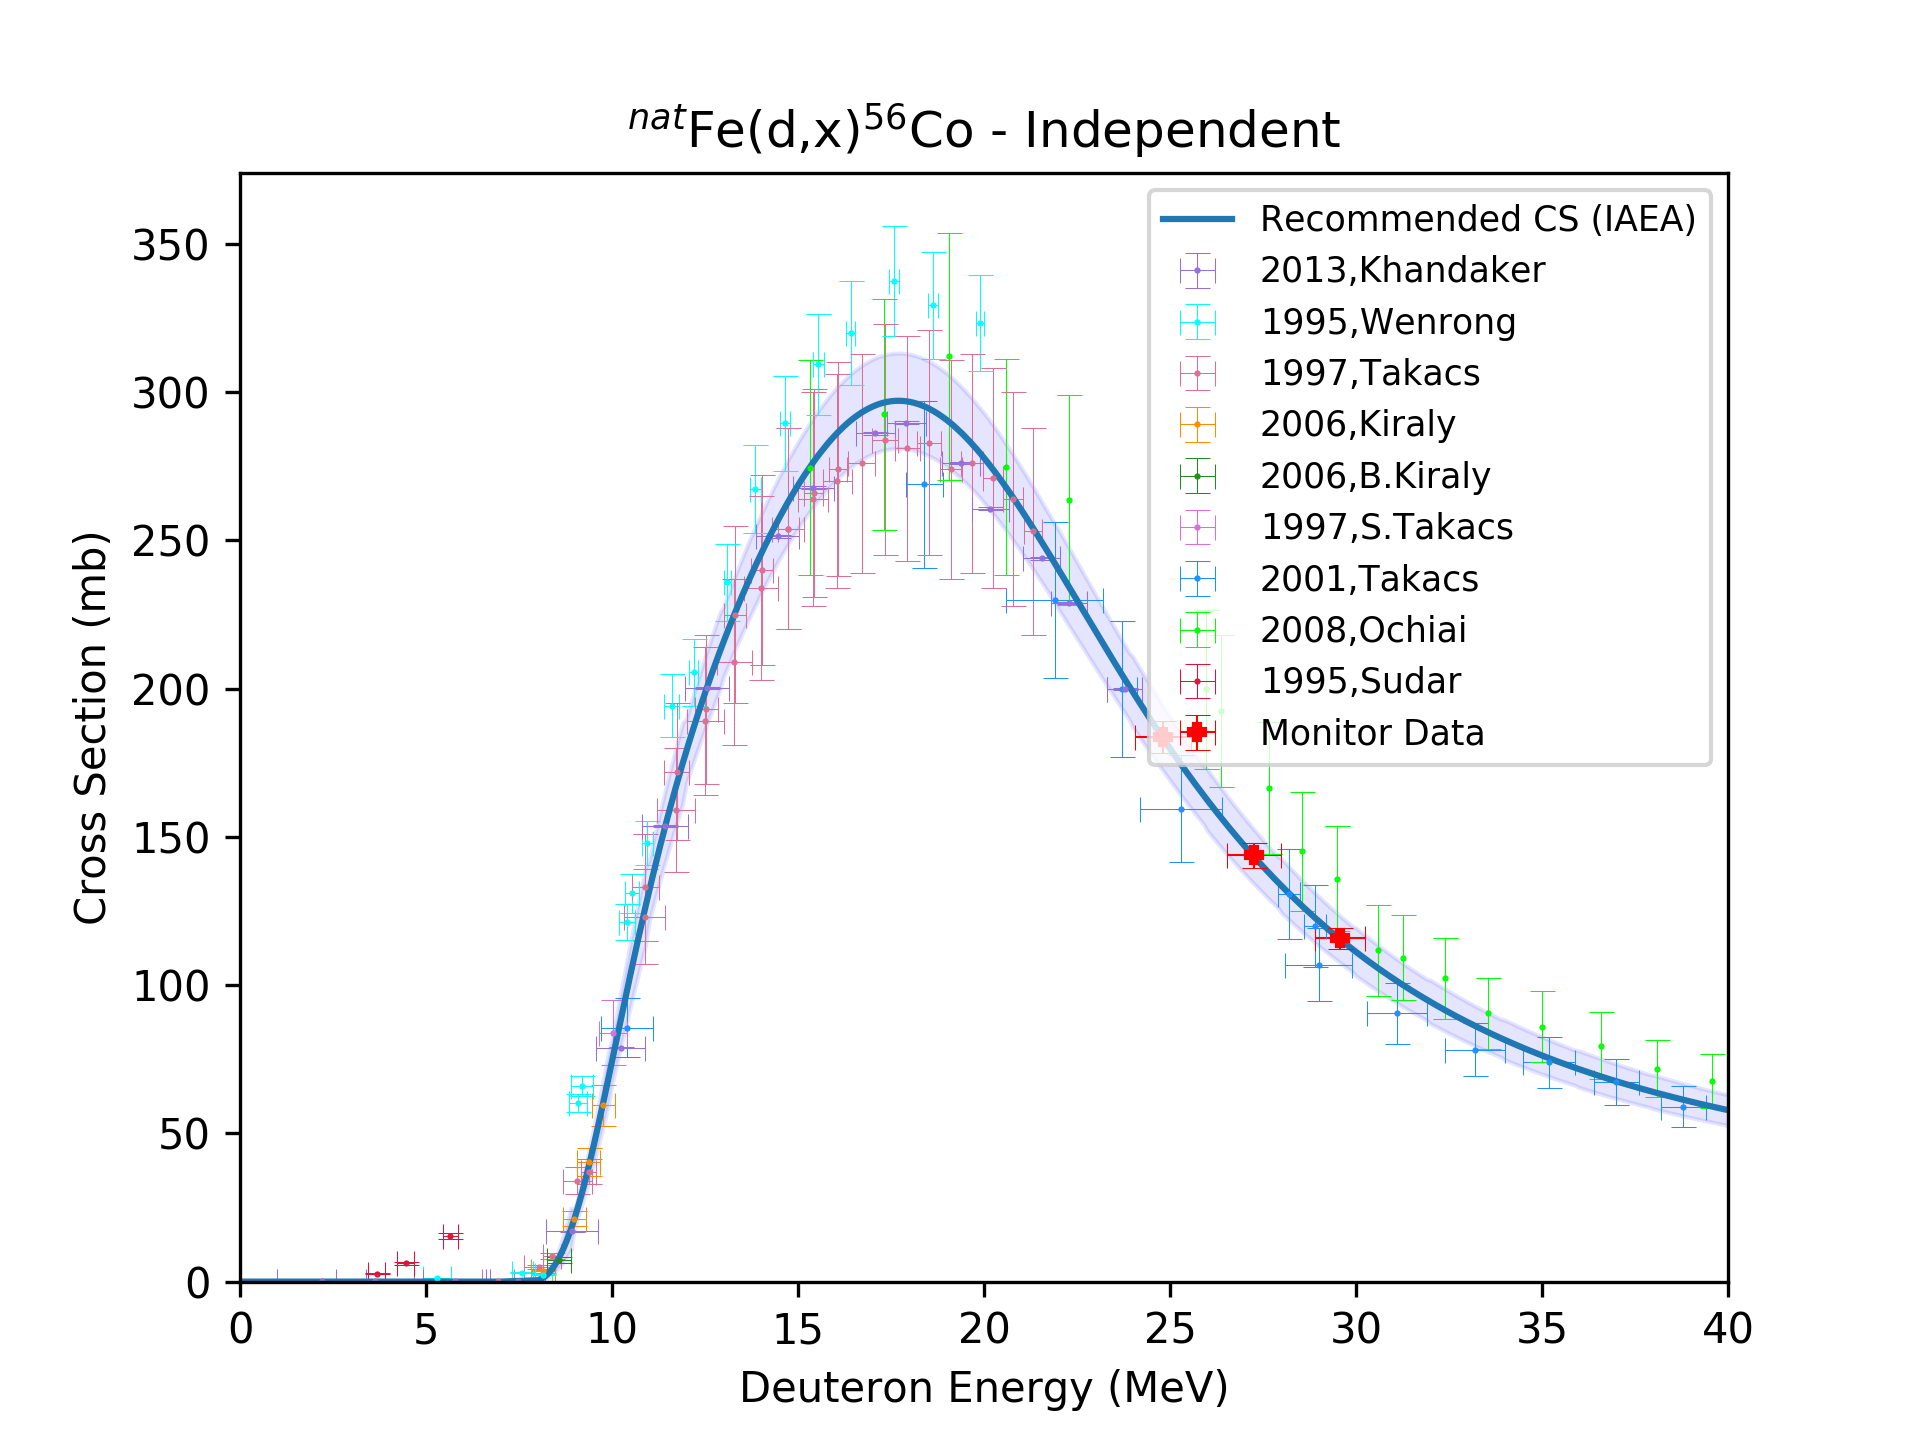
\includegraphics[width=5cm]{Fe_56Co.png} }}%
    \quad
    \subfloat[]{{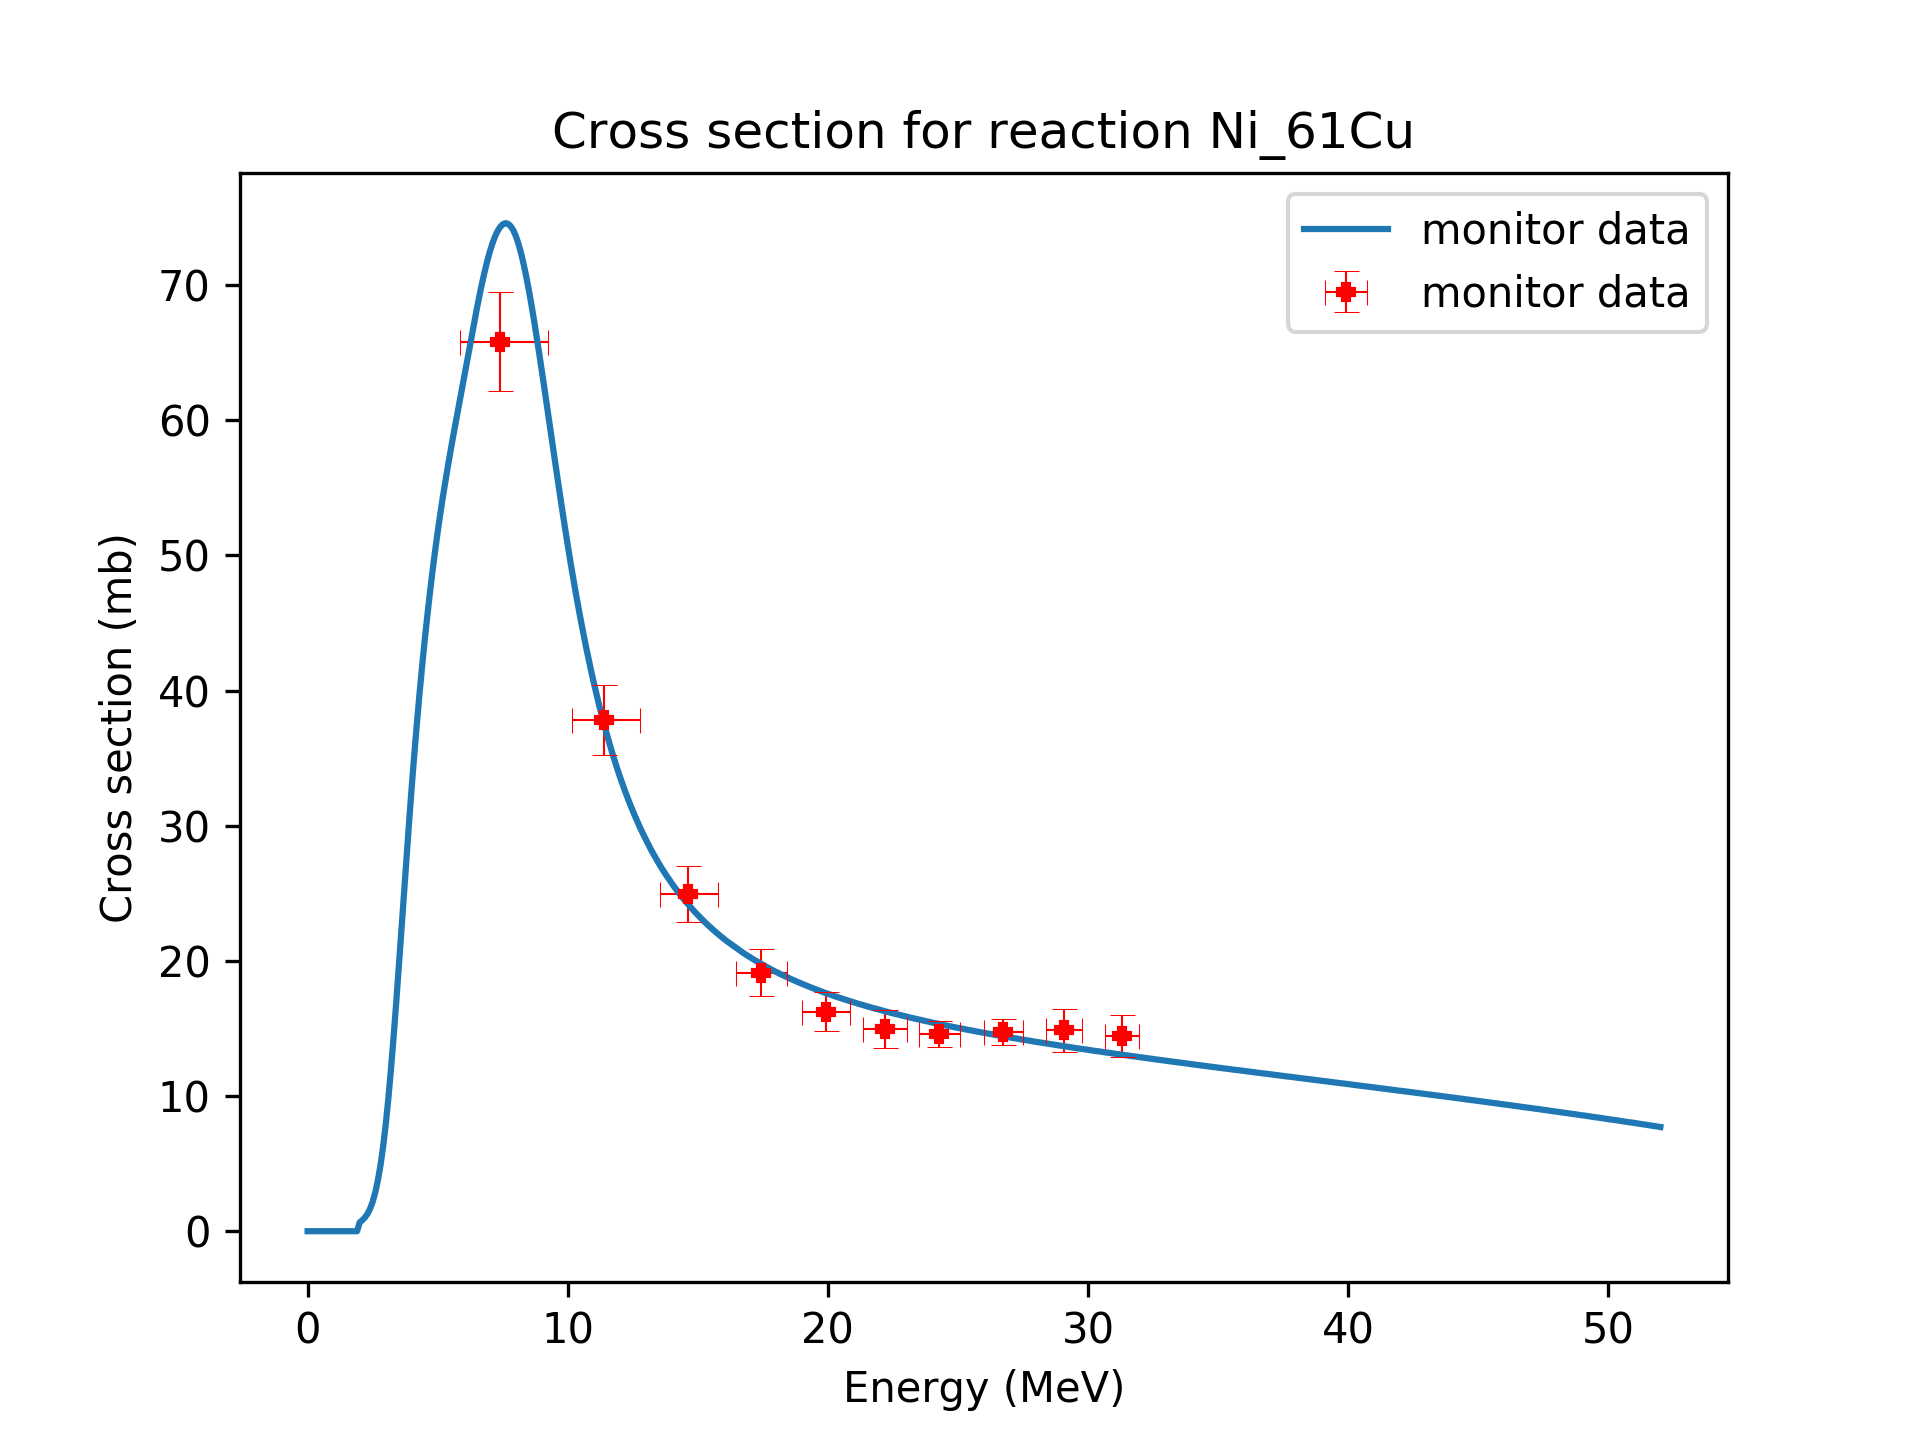
\includegraphics[width=5cm]{Ni_61Cu.png} }}%
    \subfloat[]{{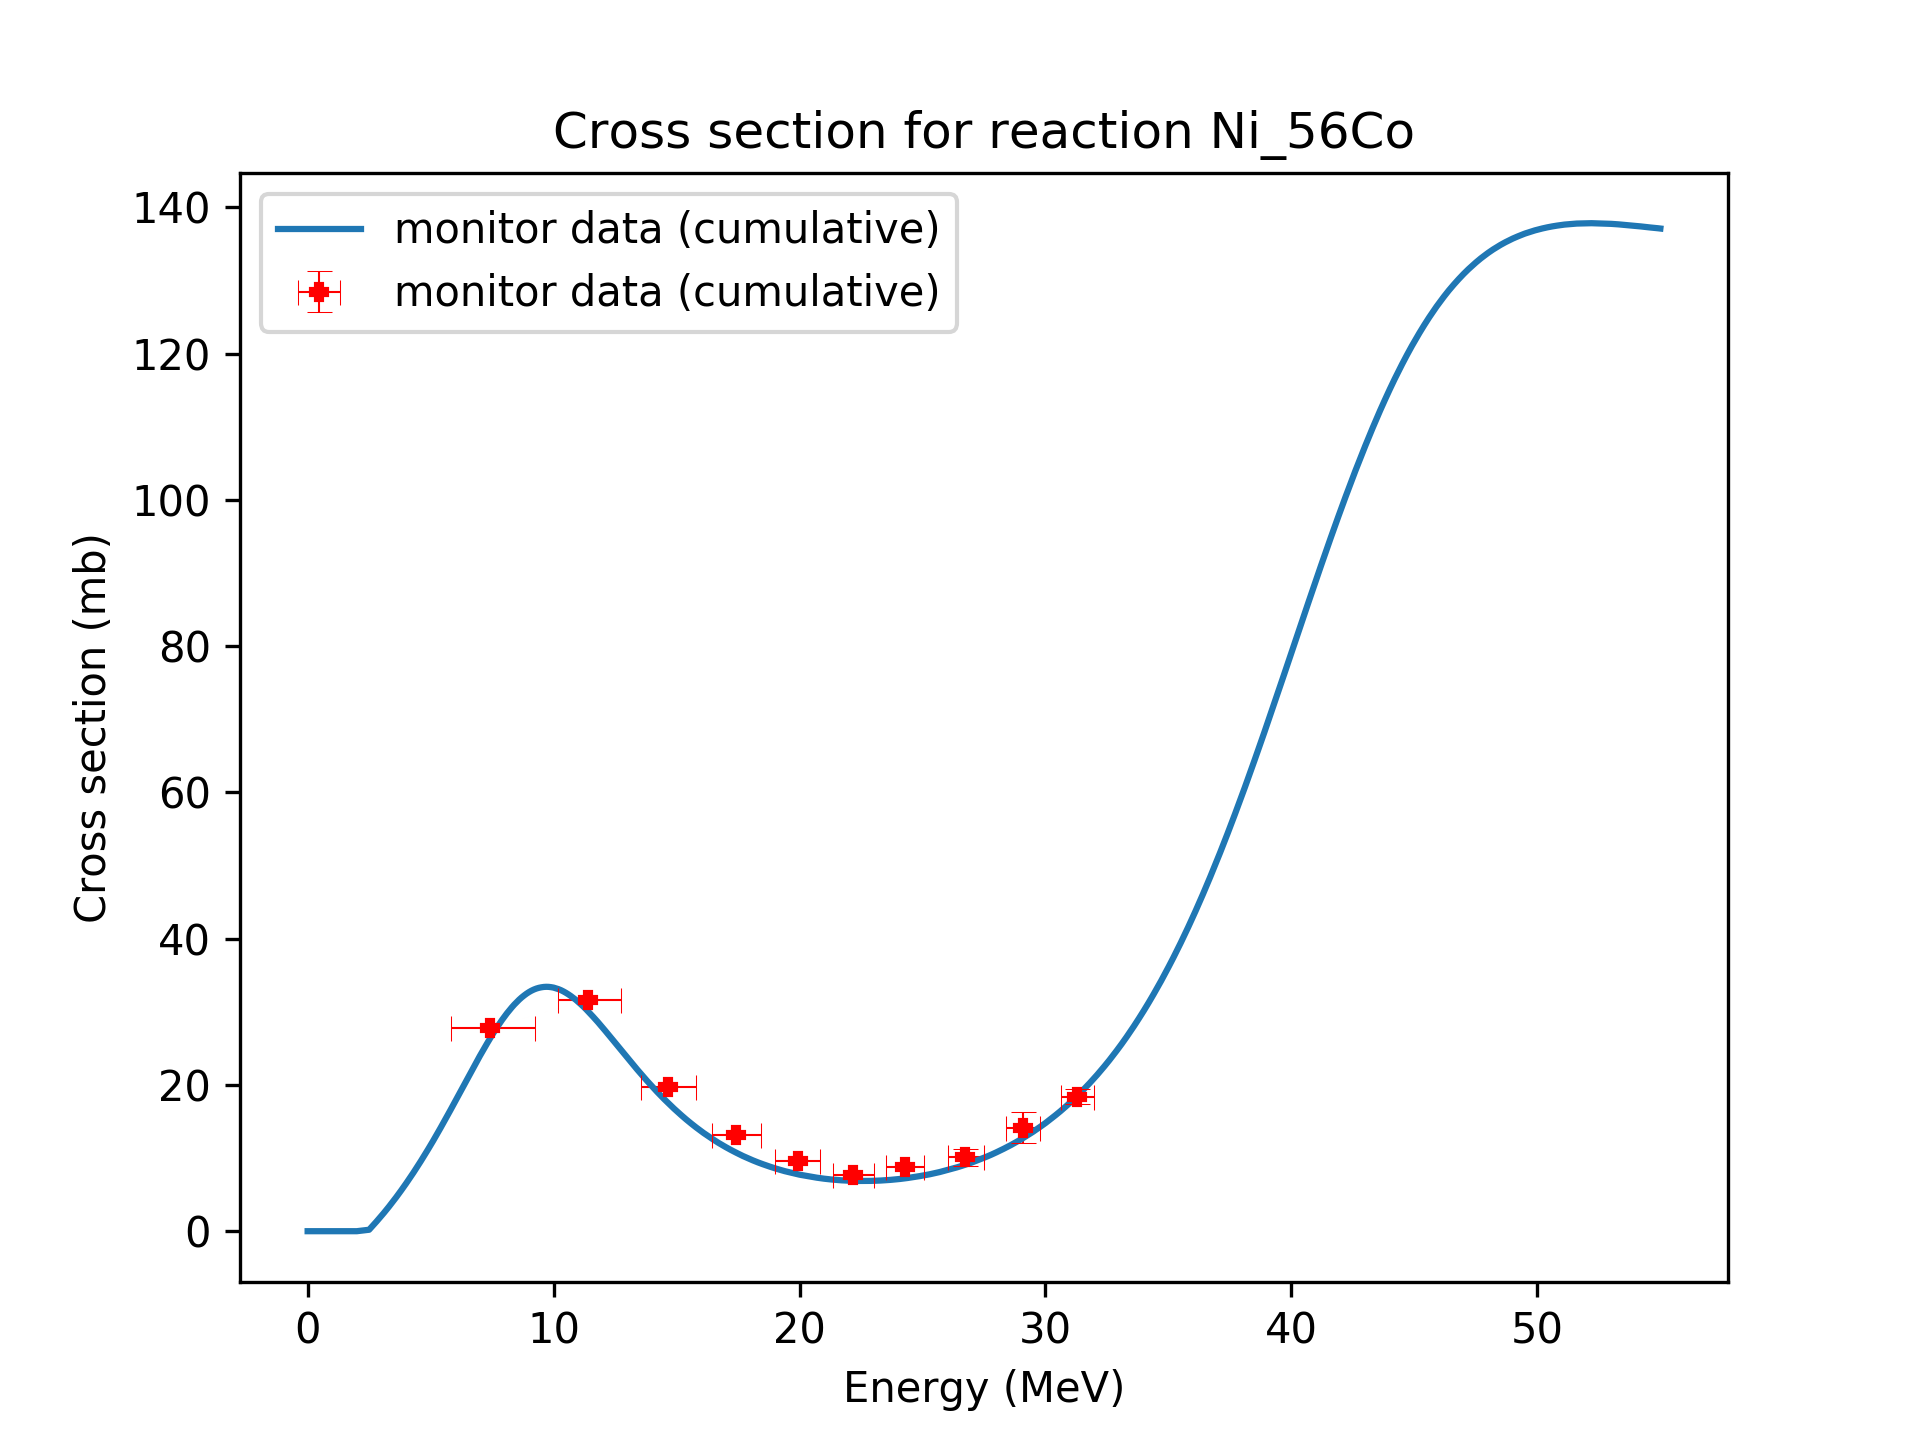
\includegraphics[width=5cm]{Ni_56Co.png} }}%
    \quad
    \subfloat[]{{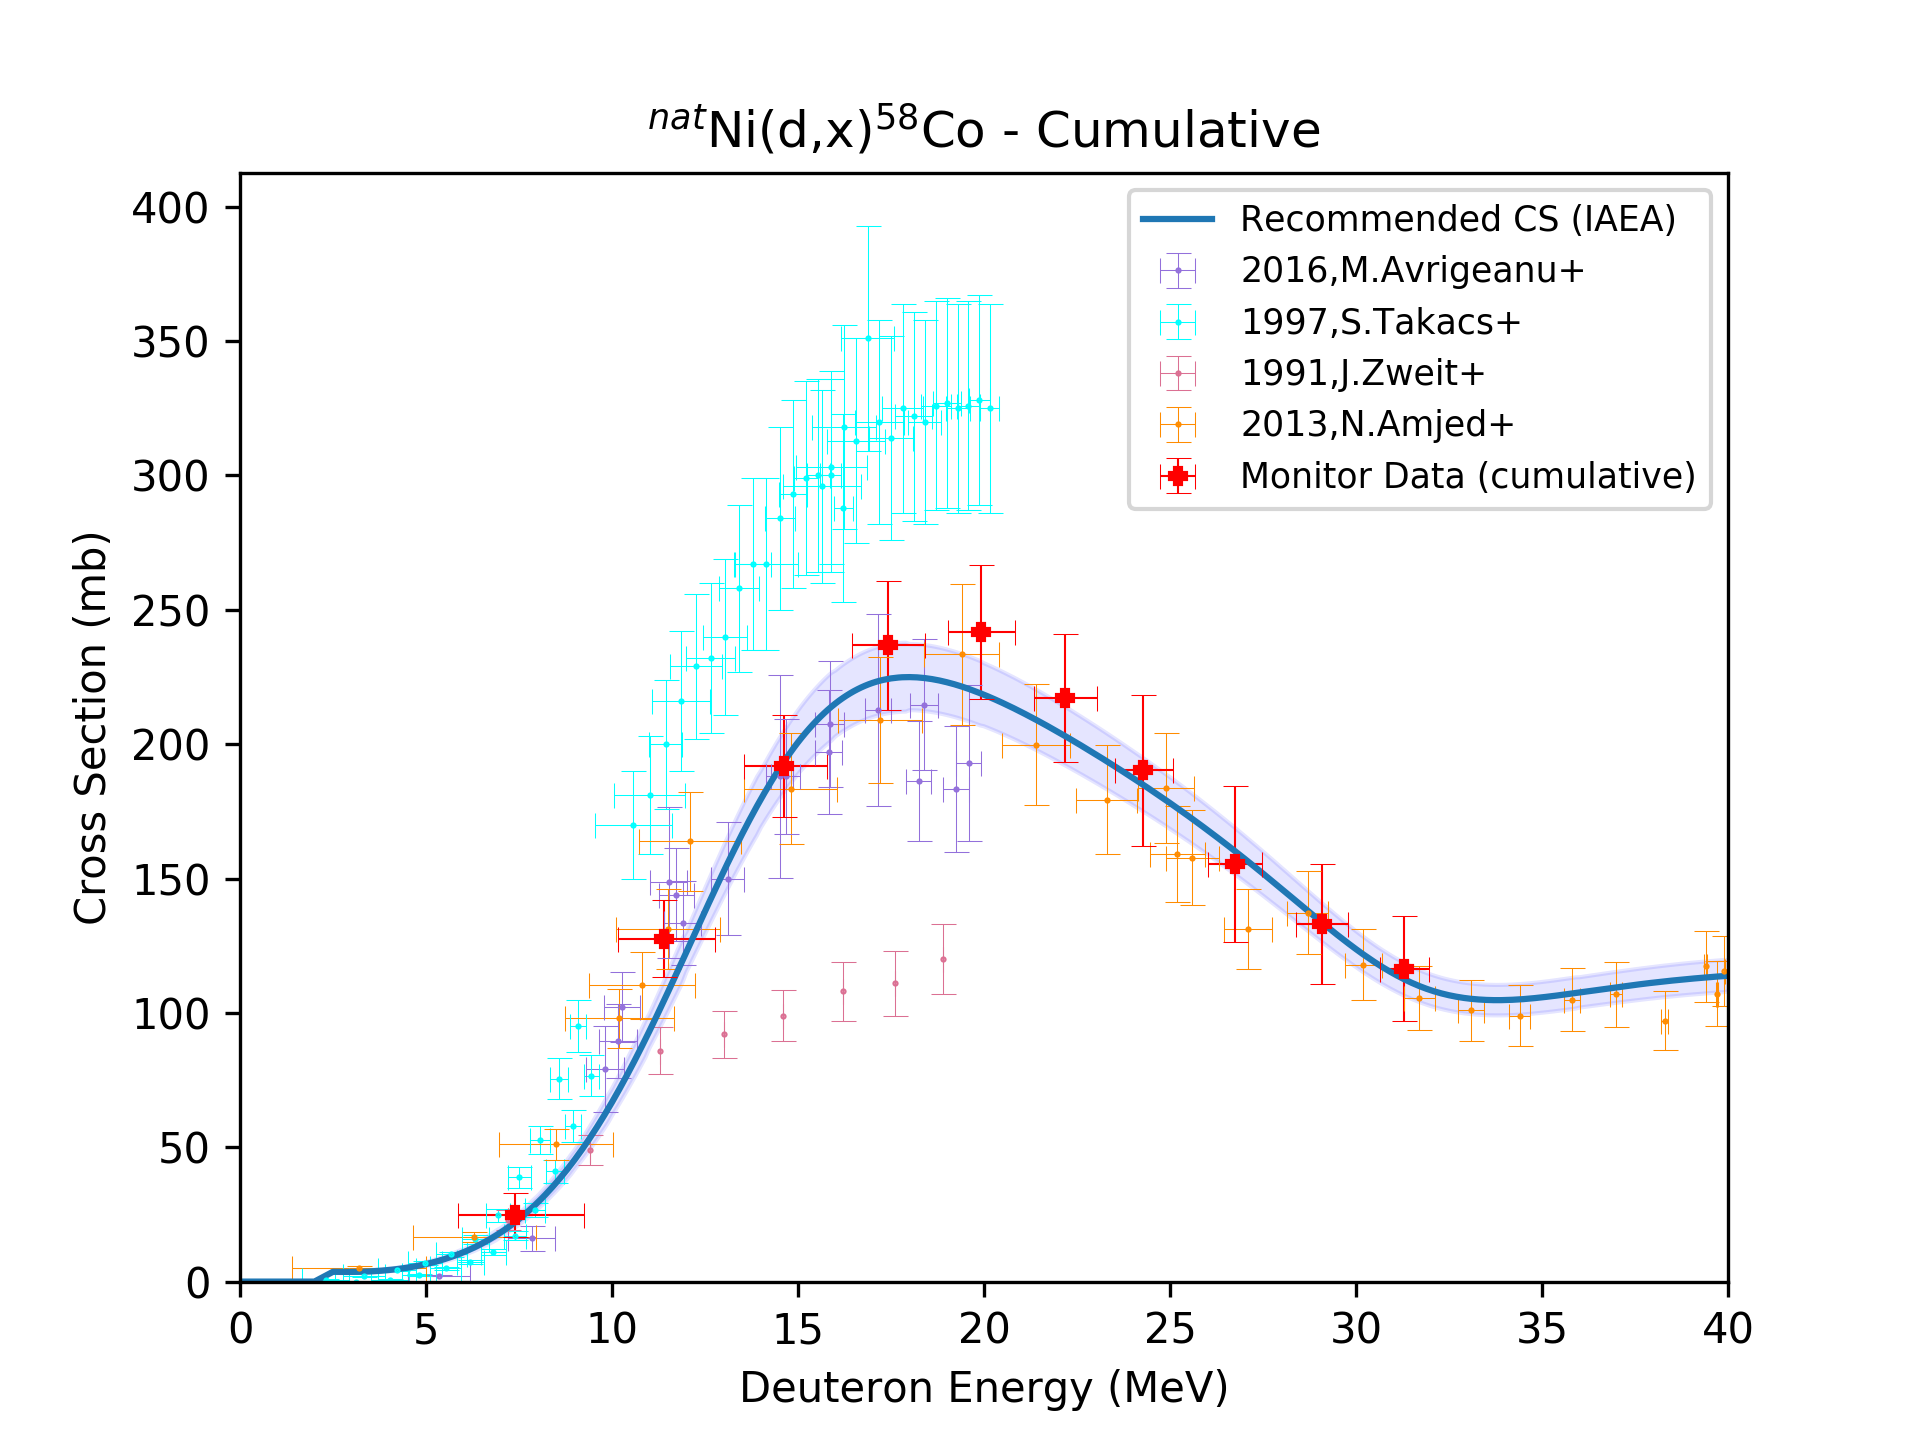
\includegraphics[width=5cm]{Ni_58Co.png} }}%
    \quad
    \subfloat[caption]{{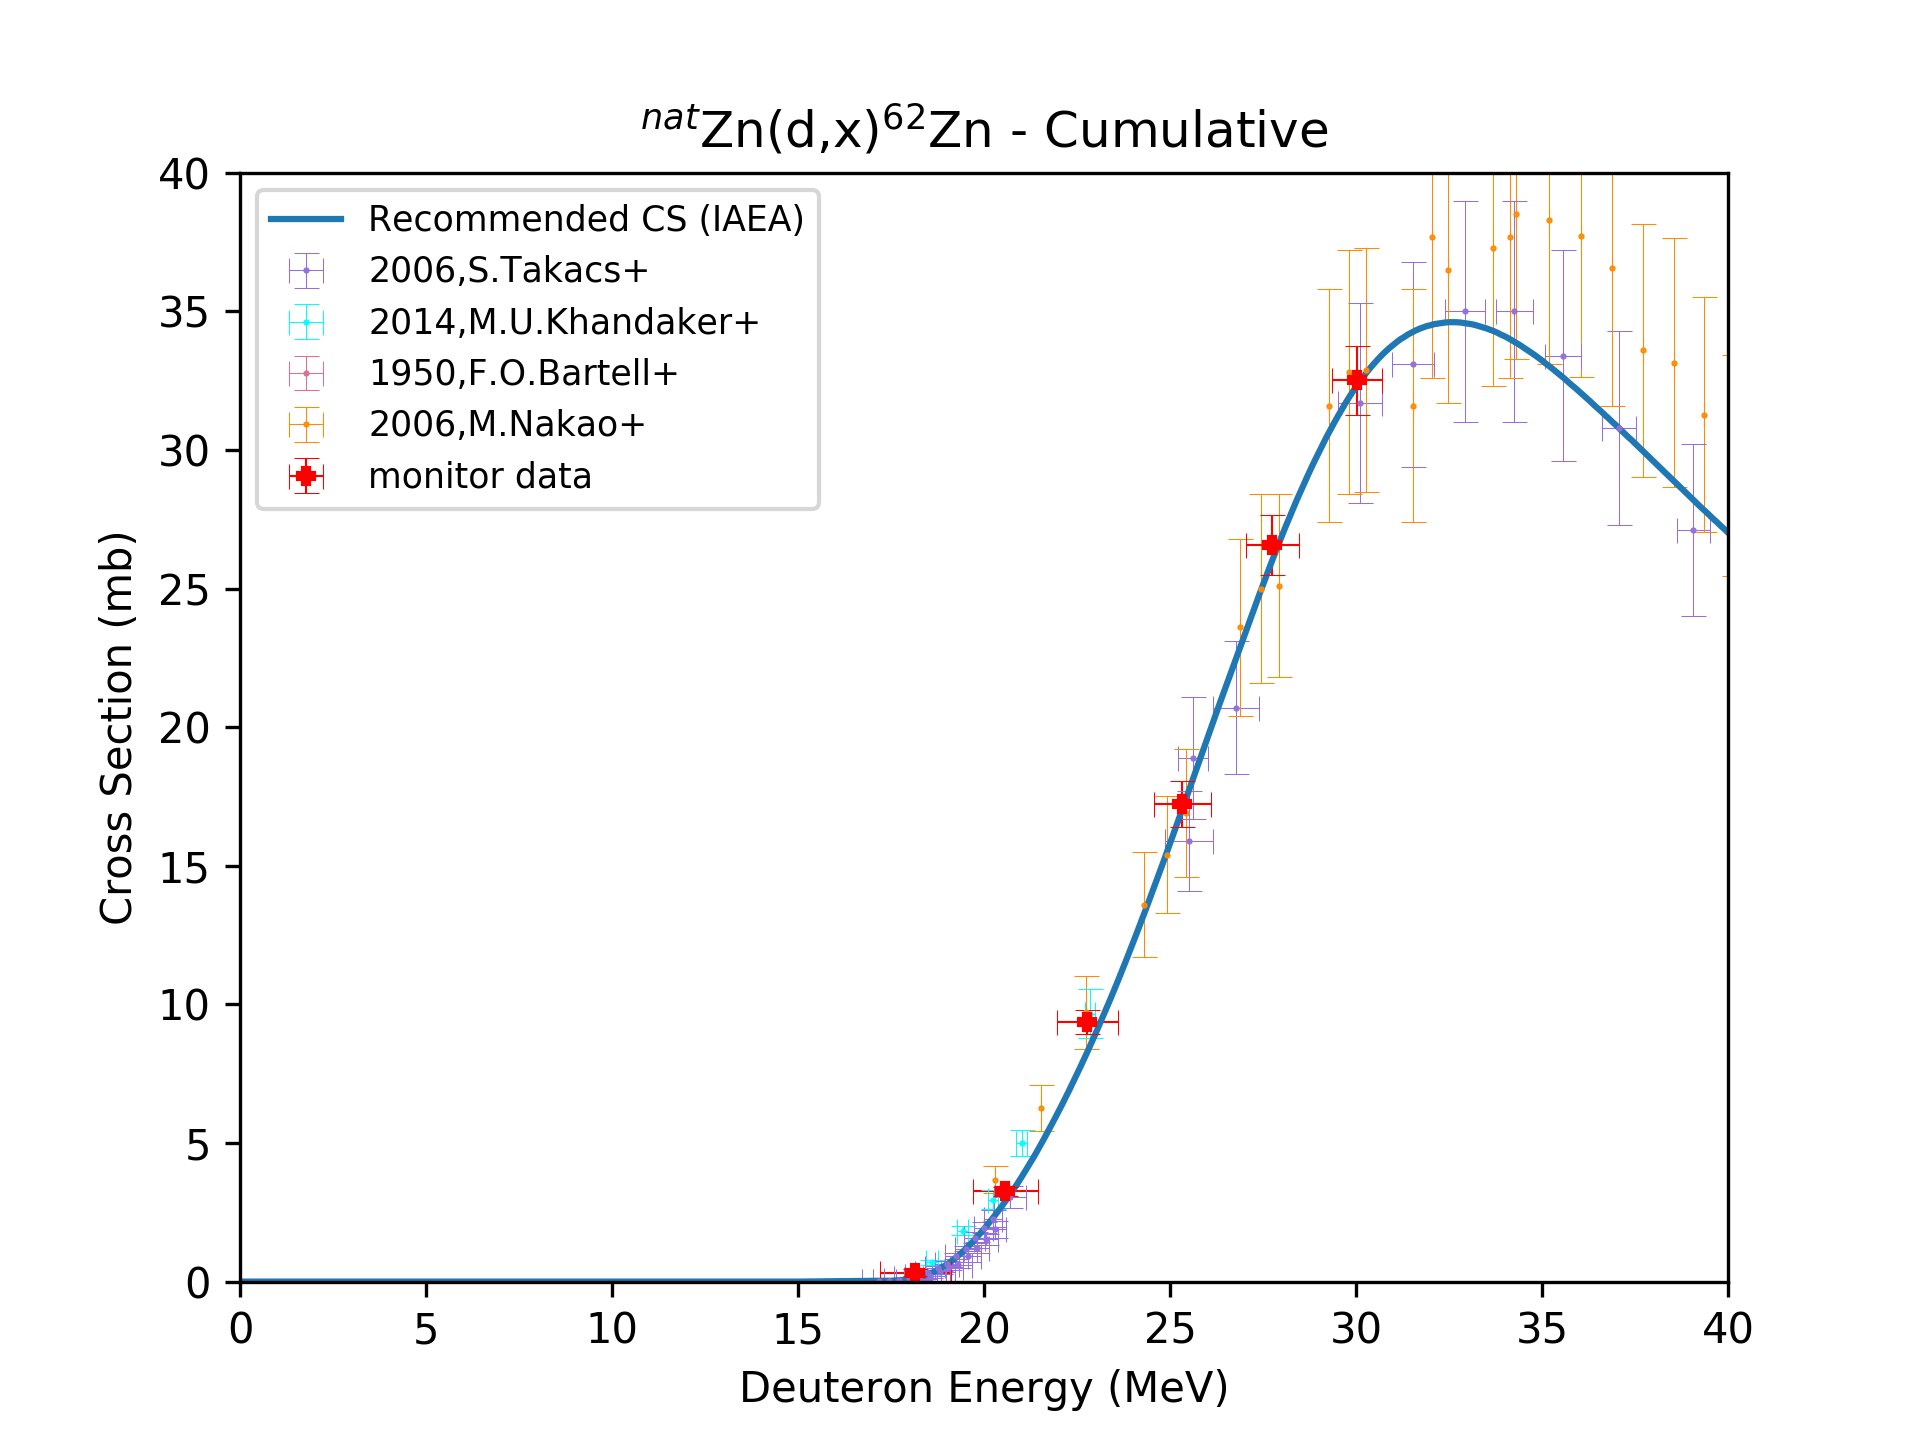
\includegraphics[width=5cm]{Cu_62Zn.png} }}%
    \quad
    \subfloat[]{{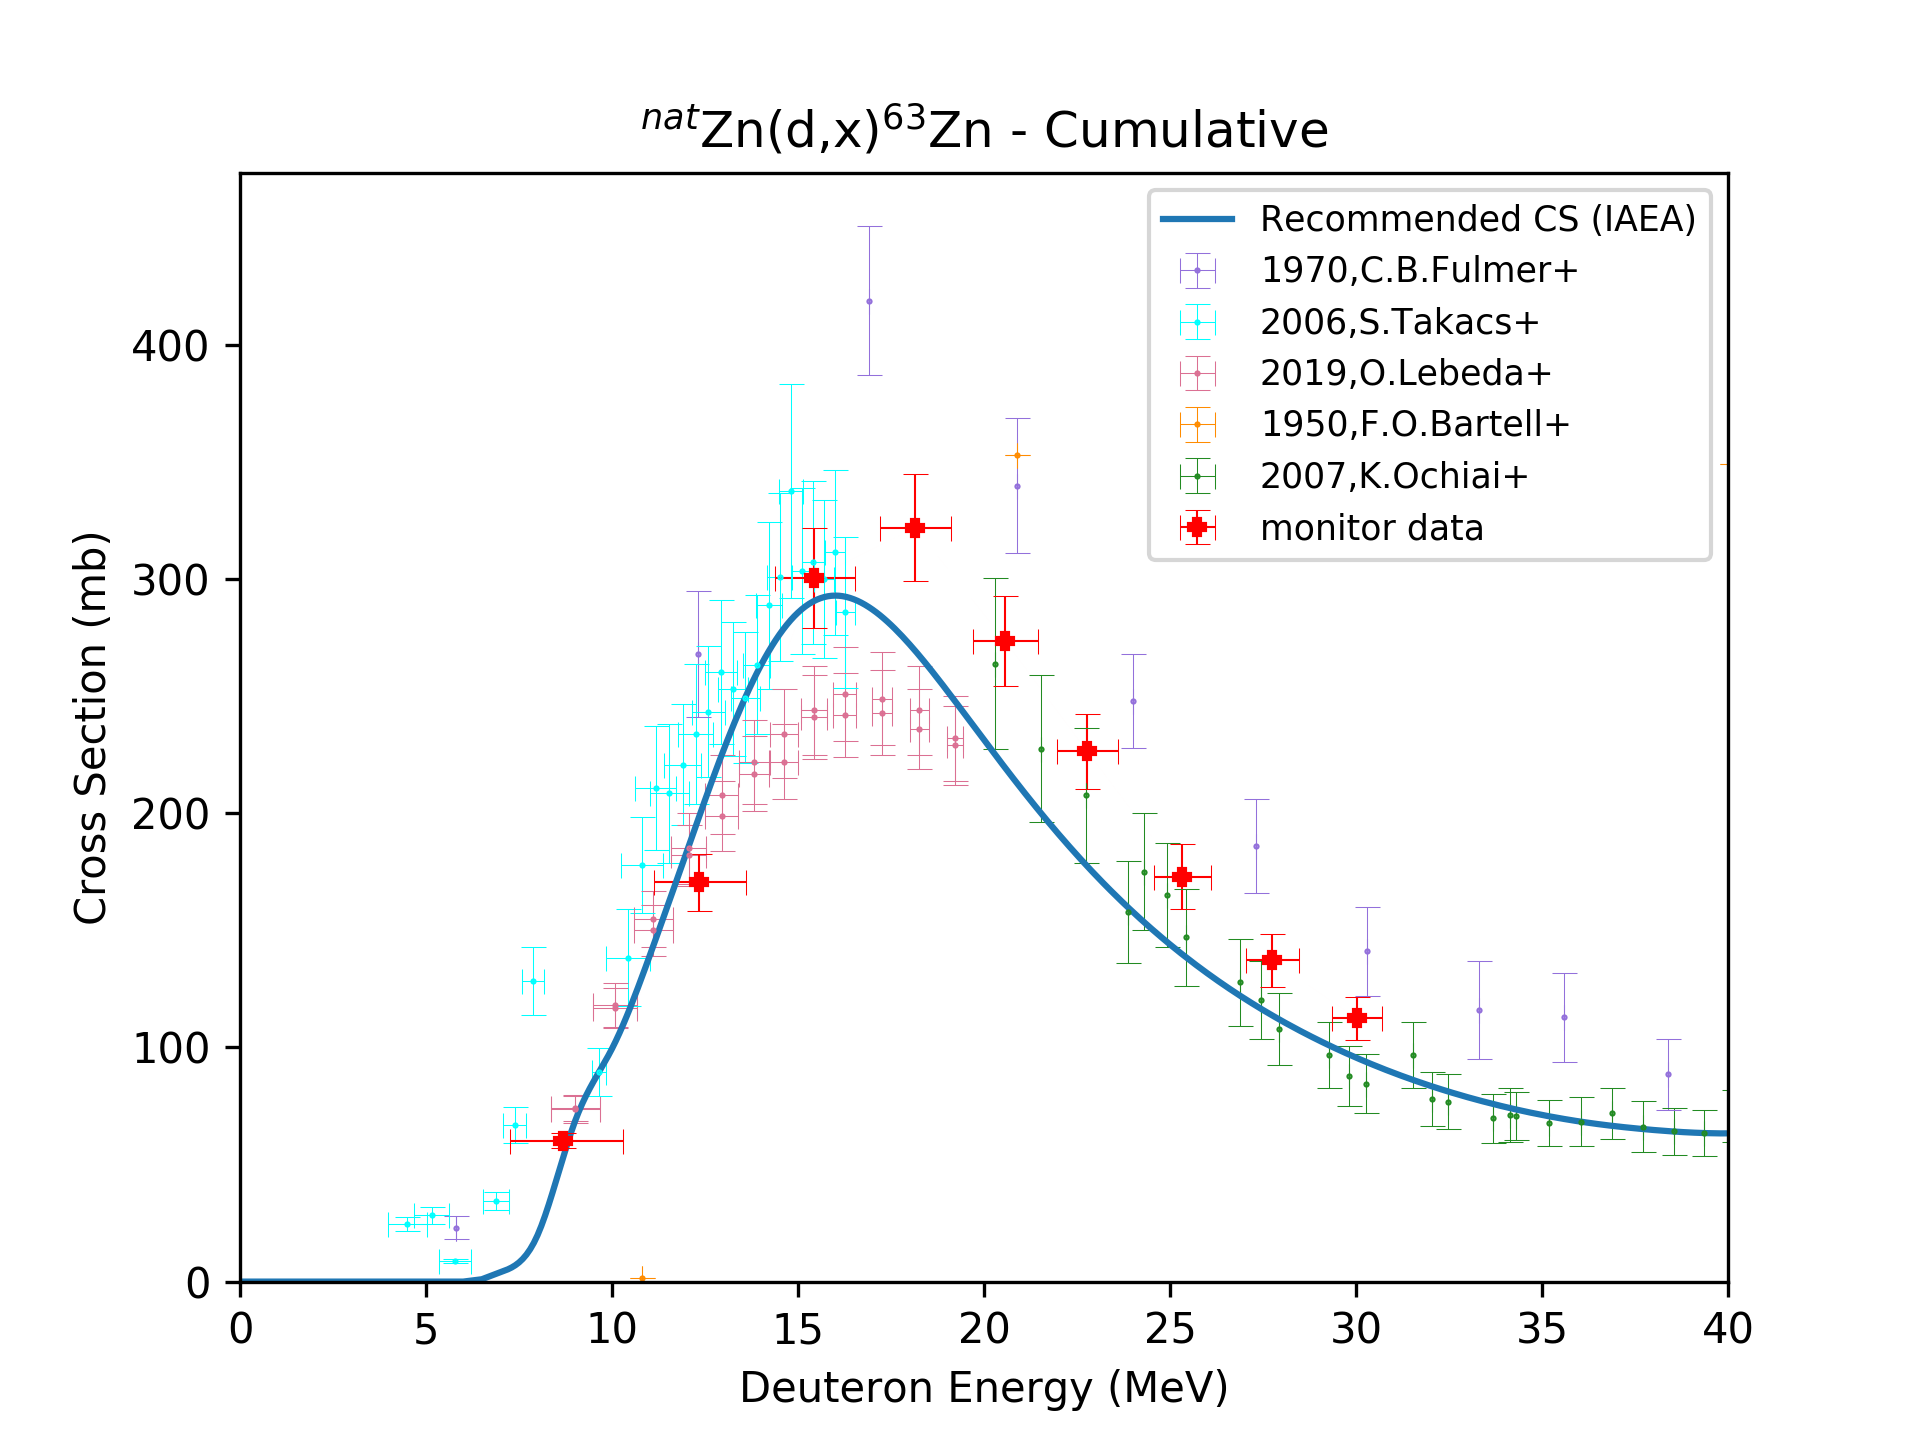
\includegraphics[width=5cm]{Cu_63Zn.png} }}%
    \quad
    \subfloat[]{{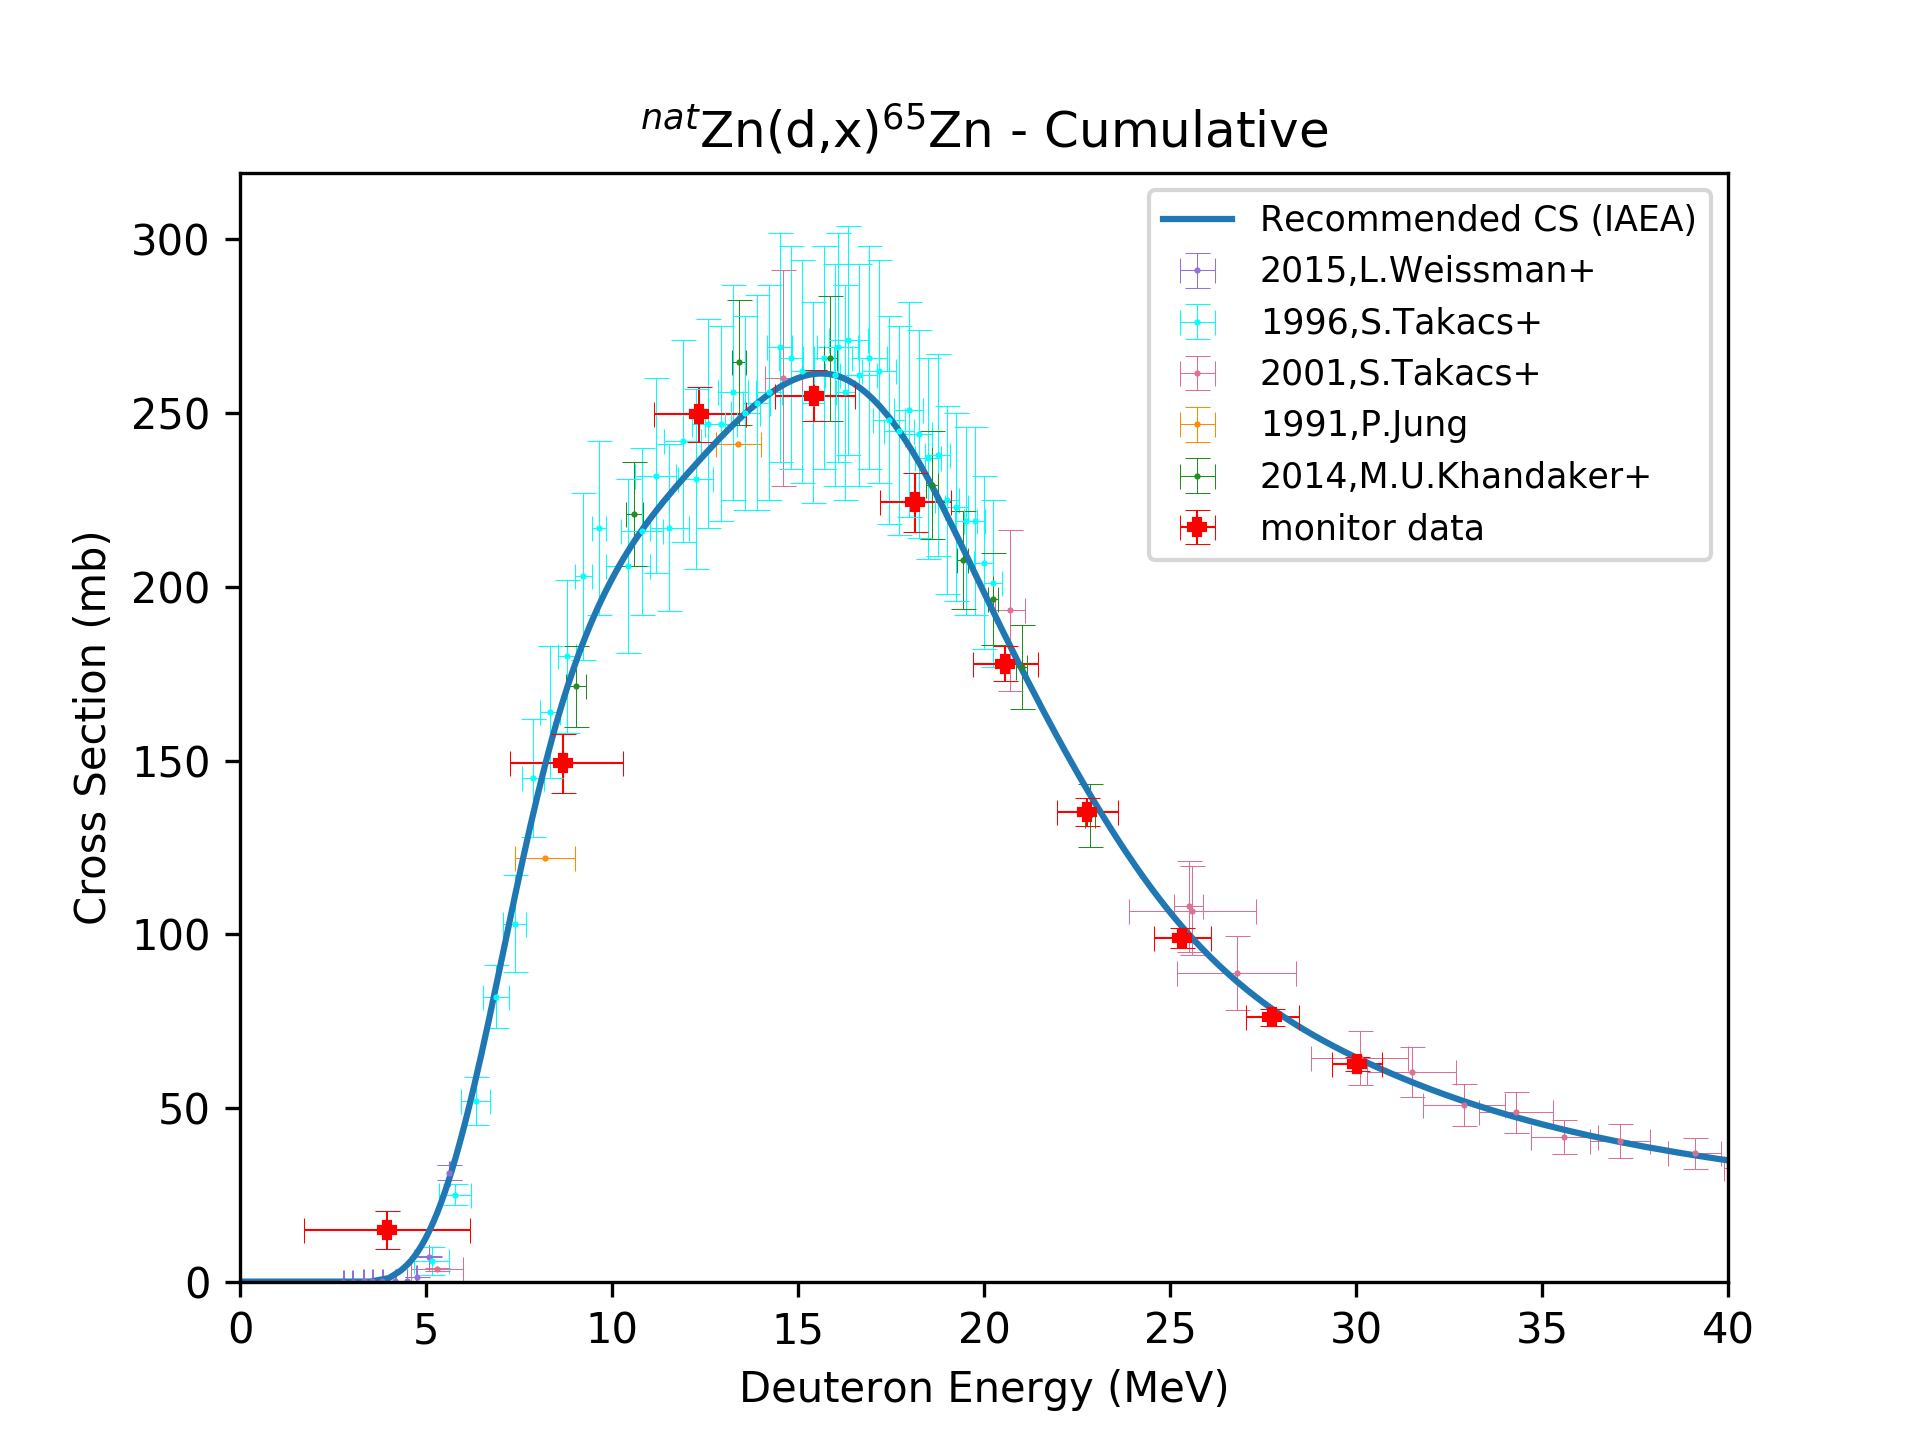
\includegraphics[width=5cm]{Cu_65Zn.png} }}%
    \quad
    \caption{Figure shows the estimation of monitor cross section using the calculated beam current. It is compared along with the monitor data.  }%
    \label{fig:monitor_BC}%
\end{figure}

\end{comment}